\documentclass[a4paper,11pt,twoside]{ThesisStyle}

\usepackage{amsmath,amssymb}             % AMS Math
% \usepackage[french]{babel}
\usepackage[latin1]{inputenc}
\usepackage[T1]{fontenc}
\usepackage[left=1.5in,right=1.3in,top=1.1in,bottom=1.1in,includefoot,includehead,headheight=13.6pt]{geometry}
\usepackage{enumerate}
\renewcommand{\baselinestretch}{1.05}

% Table of contents for each chapter
\usepackage{longtable}
\usepackage[nottoc, notlof, notlot]{tocbibind}
\usepackage{minitoc}
\setcounter{minitocdepth}{2}
\mtcindent=15pt
% Use \minitoc where to put a table of contents

\usepackage{aecompl}

% Glossary / list of abbreviations

\usepackage[intoc]{nomencl}
\renewcommand{\nomname}{List of Abbreviations}

\makenomenclature

% My pdf code

\usepackage{ifpdf}

\ifpdf
  \usepackage[pdftex]{graphicx}
  \usepackage{epstopdf}
  \DeclareGraphicsExtensions{.jpg}
  \usepackage[a4paper,pagebackref,hyperindex=true]{hyperref}
\else
  \usepackage{graphicx}
  \DeclareGraphicsExtensions{.ps,.eps}
  \usepackage[a4paper,dvipdfm,pagebackref,hyperindex=true]{hyperref}
\fi

\graphicspath{{.}{images/}}

% nicer backref links
\renewcommand*{\backref}[1]{}
\renewcommand*{\backrefalt}[4]{%
\ifcase #1 %
(Not cited.)%
\or
(Cited on page~#2.)%
\else
(Cited on pages~#2.)%
\fi}
\renewcommand*{\backrefsep}{, }
\renewcommand*{\backreftwosep}{ and~}
\renewcommand*{\backreflastsep}{ and~}

% Links in pdf
\usepackage{color}
\definecolor{linkcol}{rgb}{0,0,0.4} 
\definecolor{citecol}{rgb}{0.5,0,0} 

% Change this to change the informations included in the pdf file

% See hyperref documentation for information on those parameters

\hypersetup
{
bookmarksopen=true,
pdftitle="Towards better content dissemination applications for Disruption Tolerant Networks",
pdfauthor="Amir Krifa", 
pdfsubject="Towards better content dissemination applications for Disruption Tolerant Networks", %subject of the document
%pdftoolbar=false, % toolbar hidden
pdfmenubar=true, %menubar shown
pdfhighlight=/O, %effect of clicking on a link
colorlinks=true, %couleurs sur les liens hypertextes
pdfpagemode=None, %aucun mode de page
pdfpagelayout=SinglePage, %ouverture en simple page
pdffitwindow=true, %pages ouvertes entierement dans toute la fenetre
linkcolor=linkcol, %couleur des liens hypertextes internes
citecolor=citecol, %couleur des liens pour les citations
urlcolor=linkcol %couleur des liens pour les url
}

% definitions.
% -------------------

\setcounter{secnumdepth}{3}
\setcounter{tocdepth}{2}

% Some useful commands and shortcut for maths:  partial derivative and stuff

\newcommand{\pd}[2]{\frac{\partial #1}{\partial #2}}
\def\abs{\operatorname{abs}}
\def\argmax{\operatornamewithlimits{arg\,max}}
\def\argmin{\operatornamewithlimits{arg\,min}}
\def\diag{\operatorname{Diag}}
\newcommand{\eqRef}[1]{(\ref{#1})}

\usepackage{rotating}                    % Sideways of figures & tables
%\usepackage{bibunits}
%\usepackage[sectionbib]{chapterbib}          % Cross-reference package (Natural BiB)
%\usepackage{natbib}                  % Put References at the end of each chapter
                                         % Do not put 'sectionbib' option here.
                                         % Sectionbib option in 'natbib' will do.
\usepackage{fancyhdr}                    % Fancy Header and Footer

% \usepackage{txfonts}                     % Public Times New Roman text & math font
  
%%% Fancy Header %%%%%%%%%%%%%%%%%%%%%%%%%%%%%%%%%%%%%%%%%%%%%%%%%%%%%%%%%%%%%%%%%%
% Fancy Header Style Options

\pagestyle{fancy}                       % Sets fancy header and footer
\fancyfoot{}                            % Delete current footer settings

%\renewcommand{\chaptermark}[1]{         % Lower Case Chapter marker style
%  \markboth{\chaptername\ \thechapter.\ #1}}{}} %

%\renewcommand{\sectionmark}[1]{         % Lower case Section marker style
%  \markright{\thesection.\ #1}}         %

\fancyhead[LE,RO]{\bfseries\thepage}    % Page number (boldface) in left on even
% pages and right on odd pages
\fancyhead[RE]{\bfseries\nouppercase{\leftmark}}      % Chapter in the right on even pages
\fancyhead[LO]{\bfseries\nouppercase{\rightmark}}     % Section in the left on odd pages

\let\headruleORIG\headrule
\renewcommand{\headrule}{\color{black} \headruleORIG}
\renewcommand{\headrulewidth}{1.0pt}
\usepackage{colortbl}
\arrayrulecolor{black}

\fancypagestyle{plain}{
  \fancyhead{}
  \fancyfoot{}
  \renewcommand{\headrulewidth}{0pt}
}

\usepackage{algorithm}
\usepackage[noend]{algorithmic}

%%% Clear Header %%%%%%%%%%%%%%%%%%%%%%%%%%%%%%%%%%%%%%%%%%%%%%%%%%%%%%%%%%%%%%%%%%
% Clear Header Style on the Last Empty Odd pages
\makeatletter

\def\cleardoublepage{\clearpage\if@twoside \ifodd\c@page\else%
  \hbox{}%
  \thispagestyle{empty}%              % Empty header styles
  \newpage%
  \if@twocolumn\hbox{}\newpage\fi\fi\fi}

\makeatother
 
%%%%%%%%%%%%%%%%%%%%%%%%%%%%%%%%%%%%%%%%%%%%%%%%%%%%%%%%%%%%%%%%%%%%%%%%%%%%%%% 
% Prints your review date and 'Draft Version' (From Josullvn, CS, CMU)
\newcommand{\reviewtimetoday}[2]{\special{!userdict begin
    /bop-hook{gsave 20 710 translate 45 rotate 0.8 setgray
      /Times-Roman findfont 12 scalefont setfont 0 0   moveto (#1) show
      0 -12 moveto (#2) show grestore}def end}}
% You can turn on or off this option.
% \reviewtimetoday{\today}{Draft Version}
%%%%%%%%%%%%%%%%%%%%%%%%%%%%%%%%%%%%%%%%%%%%%%%%%%%%%%%%%%%%%%%%%%%%%%%%%%%%%%% 

\newenvironment{maxime}[1]
{
\vspace*{0cm}
\hfill
\begin{minipage}{0.5\textwidth}%
%\rule[0.5ex]{\textwidth}{0.1mm}\\%
\hrulefill $\:$ {\bf #1}\\
%\vspace*{-0.25cm}
\it 
}%
{%

\hrulefill
\vspace*{0.5cm}%
\end{minipage}
}

\let\minitocORIG\minitoc
\renewcommand{\minitoc}{\minitocORIG \vspace{1.5em}}

\usepackage{multirow}
\usepackage{slashbox}

\newenvironment{bulletList}%
{ \begin{list}%
	{$\bullet$}%
	{\setlength{\labelwidth}{25pt}%
	 \setlength{\leftmargin}{30pt}%
	 \setlength{\itemsep}{\parsep}}}%
{ \end{list} }

\newtheorem{definition}{D�finition}
\renewcommand{\epsilon}{\varepsilon}

% centered page environment

\newenvironment{vcenterpage}
{\newpage\vspace*{\fill}\thispagestyle{empty}\renewcommand{\headrulewidth}{0pt}}
{\vspace*{\fill}}

\newtheorem{theorem}{Theorem}[section]


\begin{document}

\begin{titlepage}
\begin{center}
\noindent {\large \textbf{UNIVERSITY OF NICE - SOPHIA ANTIPOLIS}} \\
\vspace*{0.3cm}
\noindent {\LARGE \textbf{DOCTORAL SCHOOL STIC}} \\
\noindent \textbf{SCIENCES ET TECHNOLOGIES DE L'INFORMATION \\ ET DE LA COMMUNICATION} \\
\vspace*{0.5cm}
\noindent \Huge \textbf{P H D\ \ T H E S I S} \\
\vspace*{0.3cm}
\noindent \large {to obtain the title of} \\
\vspace*{0.3cm}
\noindent \LARGE \textbf{PhD of Science} \\
\vspace*{0.3cm}
\noindent \Large of the University of Nice - Sophia Antipolis \\
\noindent \Large \textbf{Specialty : \textsc{Computer Science}}\\
\vspace*{0.4cm}
\noindent \large {Defended by\\}
\noindent \LARGE Amir Krifa \\
\vspace*{0.8cm}
\noindent {\Huge \textbf{Towards efficient content dissemination over disruption tolerant networks}} \\
%Towards efficient content dissemination over disruption tolerant networks
%Towards better content dissemination applications for Disruption Tolerant Networks
\vspace*{0.8cm}
\noindent \Large Thesis Advisor: Chadi \textsc{Barakat} \\
\vspace*{0.2cm}
\noindent \Large prepared at INRIA Sophia Antipolis, \textsc{Planete} Project-Team\\
\vspace*{0.2cm}
\noindent \large to be defended on Monday, April 23, 2012 \\
\vspace*{0.5cm}
\end{center}
\noindent \large \textbf{Jury :} \\
\begin{center}
\noindent \large 
\begin{tabular}{llcl}
\textit{President :}	& Christian \textsc{Bonnet}		& - & EURECOM, Sophia Antipolis, France\\
      \textit{Reviewers :}	& Jorg \textsc{Ott}	& - & COMNET, Aalto University, Finland\\
                        	& Marcelo \textsc{Dias de Amorim}		& - & LIP6, Paris, France\\
      \textit{Advisor :}	& Chadi \textsc{Barakat}	& - & INRIA, Sophia Antipolis, France\\
                        %   & Thrasyvoulos \textsc{Spyropoulos}	& - & EURECOM, Sophia Antipolis, France\\
           \textit{Examinator :}  & Thomas \textsc{Karagiannis} & - & Microsoft Research, Cambridge, UK\\
                                 & Thrasyvoulos \textsc{Spyropoulos}	& - & EURECOM, Sophia Antipolis, France \\
\end{tabular}
\end{center}
\end{titlepage}
\sloppy

\titlepage

\dominitoc

\pagenumbering{roman}

\cleardoublepage

\section*{Acknowledgments}

I would like to express my deepest gratitude to Professor Chadi Barakat, my advisor and Professor Thrasyvoulos Spyropoulos. I thank you for your continuing guidance and support during my three years of research. Your sharp sense of research direction, great enthusiasm, and strong belief in the potential of this research has been a tremendous force for the completion of this work. I have learned so many things from you. Most importantly, I thank you for encouraging me in each step of my growing path. Your strong belief in me and continuous encouragement have made this research such an exciting experience that our collaboration finally produces something that we are both proud of.

This thesis would not have been possible without the assistance of many people. I would also like to express my extreme appreciation to my thesis committee members: ... . They contributed their precious time to read my thesis, and provided valuable suggestions and comments that helped to improve the quality of this thesis. I would also like to thank my colleagues and friends at Planete team. There are many other people whose names are not mentioned here. It does not mean that I have forgotten you or your help. It is a privilege for me to work and share life with so many bright and energetic people. 

I would never get this far without the support of my parents. Thank you for always believing in me and supporting me. Your love and encouragement have been and will always be a great source of inspiration in my life.  

Meriem, my dear fiance, you are always my strength. I owe my deepest gratitude to you for your infinite patience that accompanied me along this long journey. Your love pulled me through many difficult times. 

\cleardoublepage

\section*{Abstract}
The rapid proliferation of advanced mobile devices has created a growing demand for data content. Existing approaches cannot keep up with the large volume of content generated and requested, without the deployment of new expensive infrastructure. Exchanging content of interest \emph{opportunistically}, when two nodes are in range, presents a low cost and high bandwidth alternative for popular, bulky content. Yet, efficiently collecting, storing, and sharing the content while preventing selfish users from impairing collaborative ones, poses major challenges.

In this thesis, we start by discussing the state of the art in terms of proposed solution for both point-to-point content routing and point-to-multipoint content sharing solutions in DTN(s). Our main observations were first that \emph{(i)} despite a large amount of effort invested in the design of efficient routing and content dissemination protocols for DTN, there has not been a similar focus on storage management and scheduling policies. And second \emph{(ii)}, that in addition to dealing with the resources management challenges, distributed (or peer-to-peer) content sharing systems over non-altruistic mobile devices have one more important issue to deal with: the one to ensure enough nodes collaborate to make the system interesting to participants. This latter goal is often conflicting with optimal resources management algorithms. 

Following the latter preliminary study, we tried to solve the highlighted problems in their foundations. So, we focus first \emph{(i)} on the problem of point-to-point content routing through a DTN. Such a problem is frequently encountered in environment and habitat monitoring based on sensor networks where sensor nodes try to deliver in an efficient way the collected observations and measures to a gateway node. We propose a practical and efficient joint scheduling and drop policy that can optimize different performance metrics, such as average delay and delivery probability. We first use the theory of encounter-based message dissemination to derive the optimal policy based on global knowledge about the network (GBSD, Global knowledge Based Scheduling and Drop). Then, we introduce a method that estimates all necessary parameters using locally collected statistics. Based on this, we derive a distributed scheduling and drop policy that can approximate the performance of the optimal policy in practice (HBSD, History Based Scheduling and Drop). Finally, we study how sampled statistics can reduce the \textit{signaling} overhead of our algorithm and examine its behavior under different congestion regimes. 

In a second step \emph{(ii)}, we addressed the problem of efficiently handling \emph{large scale} content sharing over non-altruistic mobile devices. Our ultimate goal was to enable people throught a channel based architecture to express their interests, head out in the real world and wait to get notified whenever a content that matches their interests is retrieved. To achieve this, we proposed MobiTrade as a candidate architecture. The latter is an utility driven trading system for efficient content sharing on top of a DTN. MobiTrade does not only take care of the network and device resources, but also carefully consider: \emph{(i)} the propagation of interests of participating users, \emph{(ii)} the matching of these interests to individual node mobility patterns, and \emph{(iii)} the willingness of involved users to collaborate. While simple tit-for-tat (TFT) mechanisms can force nodes to \emph{give one to get one}, dealing with the inherent tendency of peers to take much but give back little, they can quickly lead to deadlocks when some (or most) of interesting content must be somehow fetched across the network. To resolve this, MobiTrade relies on a \emph{trading} mechanism that allows a node \emph{merchant} to buy, store, and carry content \emph{for other nodes  (its clients)} so that it can later trade it for content it is personally interested in. To exploit this extra degree of freedom, MobiTrade nodes continuously \emph{profile} the type of content requested and the collaboration level of encountered devices. An appropriate utility function is then used to collect an optimal inventory that maximizes the expected value of stored content for future encounters, \emph{matched} to the observed mobility patterns, interest patterns, and collaboration levels of encountered nodes. 

Both of our resources management systems for point-to-point DTN routing (HBSD) and our channel based content sharing architecture (MobiTrade) have been validated respectively through extensive NS-2 and NS-3 simulations along with a multitude of synthetic mobility models and real mobility traces. Furthermore, in order to ensure the feasibility of our protocols and offer them to users, we implemented respectively HBSD and MobiTrade for the DTN2 reference architecture and on real Android powered mobile devices and did further experiments in real environments.  
\\
{\large\textbf{Keywords:}}
Resources Management, Content Dissemination Architecture, Disruption Tolerant Networks, DTN2, Android  

\tableofcontents

\mainmatter

\chapter{Introduction}
\label{chapter:Introduction}

Mobile networking is quickly reaching a tipping point. While content has been a second-class customer for cellular networks until recently, the wide spread of smart phones, and the access these provide to existing (e.g. social networking) and novel applications, are generating unprecedented amounts of mobile content. Indeed, user demand for content is increasing and creating a shift in focus towards content and content centric systems~\cite{CCN}, in both wired and wireless Internet. According to statistics published by ComScore~\cite{ComScore}, content dissemination through social networking ranks as the fastest-growing mobile content category. It was also reported that mobile content traffic exerted by mobile devices fetching content from the Internet is already a drainage of mobile operators' network resources~\cite{ATT,ATT2,Killer-DTN} . Similar to the wired Internet, mobile users are now coping with the congestion at network gateway. The capacity of current cellular infrastructures (e.g. GPRS and 3G) has already been pushed to the limit by even a small number of eager data plan users~\cite{ATT}. To support the increasing number of devices generating content at high rates, ISPs will inevitably be pushed towards either lowering bandwidth quotas~\cite{ATT}, adopting non flat rate plans, or deploying (expensive) next generation equipment (e.g. LTE). This has lead many researchers (and industry) to explore alternative or hybrid architectural solutions~\cite{CellOffLoading,Augmenting3G}. 

To this end, direct mobile-to-mobile communication can be leveraged to harvest the large amounts of unused bandwidth between wireless devices in proximity. Mobile devices with multiple wireless interfaces (e.g. Bluetooth and WiFi) allow two users in range to exchange content at much higher speeds, lower power consumption per bit, and essentially no (direct) monetary cost~\cite{Energy-Delay}. This raises an opportunity for a content dissemination overlay over the large number of mobile devices \emph{in the wild}, meeting with each other in passing. Nevertheless, users mobility and the much shorter range of high speed interfaces make \emph{contacts} between devices inherently \emph{intermittent} and \emph{time limited}. Indeed, as the topology is very unstable, content providers and content consumers might be completely unaware of each other and never connected at the same time to the same part of the network. Therefore, content should be replicated and moved towards users in a \emph{store-carry-and-forward} manner. The latter approach falls within the concept of Disruption Tolerant Networks (DTNs) that tolerate network partitions, long disconnections and topology instability in general and that consider users mobility as being the most effective way to deliver content to interested users. 

Since the DTN concept was introduced~\cite{dtnrg}, a significant share of research has focused on the design of point-to-point content routing protocols and applications like the ones dedicated for large-scale disaster recovery, ecological and ocean monitoring~\cite{Juang:zebranet, Heidemann:Acoustic}, vehicular networks~\cite{Levine:MaxProp}, and projects such as TIER~\cite{TIER}, Digital Study Hall~\cite{DSH} and One Laptop Per Child~\cite{OneLaptopPerChild} to benefit developing nations. And recently, researchers switched the focus to a second category of DTN architectures, the ones based on point-to-multipoint communication model that aims to provide complementary content dissemination solutions to the Internet based ones. 

Irrespective of the DTN application category, the uncertainty about network conditions in a disruption tolerant environment makes content routing and dissemination a challenging problem and rises many questions with regards to the management of the mobile devices resources (storage, energy, etc). Moreover, mobile devices are usually small and light equipments with limited resources (storage, battery power, limited radio range). Consequently, if an application context requires the cooperation from rational users, one should expect them to adopt selfish behaviors when deciding to replicate the content for the purpose of maximizing their revenues and conserving their resources (for example, their battery life or storage capacity). This context introduces a new class of problems for content routing and dissemination in DTN(s) which we detail in the following section.

\section{Challenges faced by content routing and dissemination in DTN(s)}

\paragraph{Mobility}

Due to frequent topology changes, network partitioning and disruption occur very often in mobile networks than in wired networks. Network partitioning severely reduces content availability when the user that holds the desired content is not in the same partition where the client users are. Replicating content
in future separate partitions before the occurrence of network partitioning can improve content availability. Content redundancy can also increase the chance for users to find the
closest content while moving. Therefore, the replication mechanism should consider all these dynamic natures of mobile networks in order to replicate content items beforehand. However, the combination of long-term storage and the, often expensive content replication, imposes a high storage overhead on wireless devices. Therefore, the replication mechanism should also take into consideration the devices storage limitation and provide the suitable management mechanisms towards delivering contents under optimal conditions. For the same reasons, when mobility results in short contacts between users, available bandwidth could be insufficient to communicate all intended contents. Consequently, efficient scheduling policies should be provided to decide which content should be chosen and forwarded first when bandwidth is limited, regardless of the specific routing algorithm used.

\paragraph{Content availability}

A disruption tolerant network may involve a large population with thousands of devices, for example, in a crowded scenario like at a stadium or in a museum. In such dense and
large network, to lookup for a content, a query sent by a client device may need to traverse a long path to reach a replica, therefore increasing the query cost and latency. Moreover, the
existence of a large number of querying devices may cause more channel interference among clients, which thus decreases considerably the available bandwidth and increases channel
access delay. High users mobility may also affect the availability of content. Thus, the replication scheme should also be designed in such way that its performance will not be greatly affected by the large number of devices and high mobility.

\paragraph{Users selfishness}

Mobile devices are controlled by rational users who are aware of the energy constraint and the cost to share and replicate content. Given this fact, one can predict that users will behave selfishly to minimize their own cost and without caring about the system side effects unless cooperation is somehow incentivized and free-riders penalized. 

\section{Contributions}

In this thesis, we start by discussing the problem of content routing in wireless environments. We describe brifely a solution (BitHoc) that we developed towards managing in an efficient way content sharing in a mobile Ad Hoc network environment (MANET) and we give an overview of the limitations that the latter solution could face in a wireless disruption prone environment. We then study the state of the art in terms of proposed solutions for both point-to-point content routing and point-to-multipoint dissemination solutions in DTN(s). Our main observations were first that \emph{(i)} despite a large amount of effort invested in the design of efficient routing and content dissemination protocols for DTN, there has not been a similar focus on storage management and scheduling policies and second \emph{(ii)}, in addition to dealing with the resources management challenges, distributed \emph{point-to-multipoint} content sharing systems over non-altruistic mobile devices have one more important issue to deal with: the one to ensure enough nodes collaborate to make the system interesting to participants. This latter goal is often conflicting with optimal resources management algorithms. 

Starting from the latter preliminary study, we wanted to solve the highlighted problems in their foundations. In a first direction, we focus on the problem of point-to-point content routing through a DTN. Such a problem is frequently encountered in environment and habitat monitoring based on sensor networks where sensor nodes try to deliver in an efficient way the collected observations and measures to a gateway node. We develop a theoretical framework based on Epidemic message dissemination~\cite{haas:mobihoc03,Inria:MessageDelay,akis:mobihoc06}, and propose a \emph{greedy} optimal joint content scheduling and storage management policy, GBSD (Global knowledge Based Scheduling and Drop)~\cite{KrifaBS08, HBSDDTN2}, that can either maximize the average delivery rate or minimize the average delivery delay in the context of a congested delay tolerant network. GBSD derives a per-message utility by taking into account all information that are relevant for message delivery, and manages messages accordingly. Yet, to derive these utilities, it requires \textit{global} network information, making its implementation difficult in practice, especially given the intermittently connected nature of the targeted environments. In order to amend this, we propose a second policy, HBSD (History Based Scheduling and Drop)~\cite{KrifaBS08, HBSDDTN2}, a distributed (\textit{local}) algorithm based on statistical learning. HBSD uses network history to estimate the current state of required (\textit{global}) network parameters and uses these estimates, rather than actual values (as in GBSD), to calculate message utilities for each performance target metric. Furthermore, we look deeper into our distributed statistics collection solution and identify the available trade-offs between the collection overhead and the resulting performance. Aggressively collecting statistics and exchanging them with every encountered device allows estimates to converge faster (and thus achieves good performance), but it can potentially result in high energy and bandwidth consumption, and can also interfere with data transmissions. Our results suggest that close to optimal performance can still be achieved even when the signaling overhead is forced (through sampling) to take only a small percentage of the contact bandwidth. Finally, in this direction, we examine how our algorithm behaves under different congestion regimes. Interestingly, we find that at low to moderately congested regimes, the optimal policy is simply equivalent to dropping the message with the oldest age (similarly to the findings of~\cite{QueuingPolicies}), while at highly congested regimes, the optimal policy is not linear with message age; some young messages have to be dropped, as a means of indirect admission control, to allow older messages to create enough replicas and have a chance to be delivered. Hence, our framework can also explain what popular heuristic policies are doing, in this context, with respect to the optimal one.

In a second direction, we address the problem of efficiently handling \emph{large scale} content sharing over non-altruistic mobile devices. Our ultimate goal is to enable people throught a channel based architecture to express their interests, head out in the real world and wait to get notified whenever a content that matches their interests is retrieved~\cite{CCN, MobiCent, IADTN, MoB, OptimalChannelChoice, ContentPlace, SocialCast2, SocialCast, BlueTorrent, TACODTN, Peoplenet}. To achieve this, a candidate architecture should not only take care of the network and device resources, but also carefully consider: \emph{(i)} the propagation of interests of participating users, \emph{(ii)} the matching of these interests to individual node mobility patterns, and \emph{(iii)} the willingness of involved users to collaborate. This latter point can be a major deal-breaker in any envisioned architecture (as is the case for example in traditional MANETs~\cite{NashEquilibria}). As an answer to the latter challenges, we propose MobiTrade, an interest driven content dissemination architecture for opportunistic networks. MobiTrade optimizes the content sharing strategy from the perspective of each individual participant. First, we argue that Tit-For-Tat (TFT) should be directly employed in order to isolate free-riders and create incentives for nodes to share their resources. This latter point is of key importance as TFT gives content of non-direct interest monetary value. If a node $B$ has content that $A$ is interested in, but $A$ does not have something to give back, $A$ has the incentive to fetch something for $B$. $B$ now retrieves content that would otherwise be inaccessible to it, and $A$ retrieves content that is easily accessible but that it couldn't \emph{afford} before. While TFT is well known both in P2P~\cite{BitHoc} and opportunistic networks~\cite{BarterDTN} communities, it does not answer itself \emph{how mobile devices should optimally (re-)act in the presence of TFT} towards maximizing their revenues. MobiTrade answers this question by introducing a content utility framework that aims to \emph{maximize the expected future exchange value of the content inventory stored by each node}. Intuitively, the value of a piece of content to a node $A$ should depend on \emph{(i)} how many nodes are interested in it, \emph{(ii)} how often does $A$ see these nodes, \emph{(iii)} how much content, interesting to $A$, do these nodes have and \emph{(iv)} how \emph{well-behaved} are these nodes. MobiTrade uses a simply, robust utility function that implicitly captures all these features, without explicitly measuring each one, and that turns each node into a \emph{merchant} fetching the content that has the highest chance to be sold (and exchanged for content of interest) to its good \emph{clients}. Summarizing, our major contributions in this direction are:
\begin{enumerate}
    \item We formulate the optimal content sharing problem in DTNs from the perspective of non-altruistic nodes while relying on a tit-for-tat mechanism to isolate free-riders.
    \item We propose MobiTrade, a utility-based solution to this problem that predicts the (exchange) value of each piece of content and provides a customized resource allocation strategy for each node, \emph{matched} to its own interests and mobility pattern.
\end{enumerate}
To our best knowledge, MobiTrade is the first content sharing system for DTNs that can both deal with rational and selfish users while at the same time achieving good global outcomes \emph{without explicit hard constraints on the topology and dependency of nodes on their social behavior}. 

The performance evaluation of our two main contributions GBSD/HBSD and MobiTrade is done respectively through extensive NS2 and NS3 simulations supplied by real mobility traces. In Chapter~\ref{chapter:HBSD}, we implement HBSD, a real external router for the DTN2~\cite{HBSDDTN2} reference architecture. The proposed router runs on top of the DTN2 forwarding block, collects and analyses the network history towards approximating network level parameters and providing the right content drop or scheduling decisions to apply in case of a device storage congestion or a contact disruption. We also describe in Chapter~\ref{chapter:MobiTrade}, the implementation of our channel based content dissemination architecture, MobiTrade, for smart-phones equipped with the Android operating system. 

\section{Organization}

The remainder of this thesis is organized as follows. In the next chapter we introduce our problems background and discuss a list of related works. Chapter~\ref{chapter:ptp} describes the 
greedy optimal solution that we propose for point-to-point content routing within a disruption tolerant network. Chapter~\ref{chapter:HBSD} details the implementation issues of our History Based Scheduling and Drop (HBSD) content dissemination schema as an external router for the DTN2 reference architecture. In Chapter~\ref{chapter:PTMP}, we present MobiTrade, our point-to-multipoint interest driven content sharing architecture for DTN. Then, we provide in Chapter~\ref{chapter:MobiTrade} a detailed implementation analysis of MobiTrade for smartphones equipped with the Android platform. In Chapter~\ref{chapter:conclusions}, we conclude the results of our study and outline the direction for our future work.

\chapter{Background}
\label{chapter:background}
\minitoc

Content sharing is currently a universal concern among computer users and has recently become an important requirement for mobile devices. Indeed, thanks to the efficient wireless connectivity offered by mobile devices, users are frequently brought to locate and share content of interest (photos, videos, etc) with other members of the same spontaneous community. Depending on the use case, the latter spontaneous community can be considered as either a mobile ad hoc network (MANET) where by definition it is always possible to find end-to-end paths between communicating u and thus support end-to-end semantics of existing transports and applications. Or, the mobile user can belong to a larger spontaneous community, namely a delay tolerant network (DTN). The latter networking architecture offers support for communication scenarios where nodes are sparse and the contacts between them are short-lived, e.g., due to high node mobility. The DTN approach allows the intermediate nodes to store messages for extended period of time (i.e., carry), and to deliver messages towards destination when opportunity to forward a message becomes available. Thus, in contrary to MANET approach, the DTNs can deliver messages also when instantaneous end-to-end path between the nodes does not exist. 

With current technologies, users are mainly using point-to-point basic connections, which can be considered as an efficient solution when the number of users interested in the sharing session is very small and that there is no risk of connexion disruption. However, even with a guaranteed wireless connection and in the case of a large community (for example, mobile device users assisting to a conference and willing to share some papers), one is facing the following problem: increasing the number of parallel point-to-point communications may decrease the global Ad Hoc network capacity, while increasing dramatically the download time. The multi-hop point-to-point communication over long paths is also a serious issue. Therefore, there is a strong need to organize the communication overlay among devices in a way to distribute fairly the burden of content sharing among the set of participants while aiming to decrease the global download time. P2P file sharing solutions are good candidates for such infra-structureless networks (MANET) as they are based on multi-sourcing which balances resource consumption among users and reduces the dependency on any central entity. But unfortunately, P2P content sharing applications developed for the Internet cannot directly be plugged and used into mobile devices. Indeed, on one hand, these solutions are not adapted to the constraints of multi-hop wireless networks. For example, it is known that in a resource constrained environment, the choice of the users to whom to connect cannot be done independently of information on the underlying dynamic topology. Moreover, centralized users management approaches like the centralized tracker used in BitTorrent do not perform well in such environment as the tracker can be either far away or even invisible by some users because of disconnections. Furthermore, computer users rely on Internet search engines and dedicated desktop applications to look for the content they are willing to share. This approach becomes obsolete in the case of a spontaneous MANET based community and thus, a dedicated distributed content discovery approach must be provided. 

Then, if we consider a more general/challenging mobile environment where the topology is unstable and users' contact can be disrupted frequently (for example, mobile devices users moving in the street), users cannot rely any more on the content dissemination systems proposed for conventional MANETs~\cite{BitHoc}~\cite{BlueTorrent}. Indeed, the later ones are built based on the assumption that the network path are almost stable and that content providers and content consumers are connected to the same part of the network at the same time. Therefore, they are not suitable for disruption tolerant environment. From this perspective and to allow some services to operate even under
these challenging conditions, researchers have proposed a new networking paradigm, often referred to as Disruption Tolerant Networking, based on the store-carry-and-forward routing principle. Devices there, rather than dropping a session (and respectively packets) when no forwarding opportunity is available, store and carry
content until new communication opportunities arise. 

This chapter describes the background behind our work. At first hand, we discuss \emph{briefly} content sharing challenges in MANETs. We focus on P2P content sharing solutions and we give an overview of \emph{BitHoc}, the P2P open-source standalone content sharing solution that we proposed and developed for MANETs. We then discuss the reasons that could prevent users from adopting BitHoc as a content dissemination solution in the context of a disruption tolerant environment. At second hand, we focus on the \emph{main context} of this thesis, namely content sharing in a DTN environment, we study in details already existing solutions for content sharing in a disruption tolerant environment (both point-to-point content routing and point to multi-point routing protocols), we detail the limitations of the different proposed approaches and we discuss those we are able to overcome through the solutions we are proposing in this thesis. 

\section{Content sharing in MANETs}

\subsection{MANETs}

Nowadays, wireless networks have become more and more popular as they are easily deployable. These networks play a crucial role among computer networks, since they offer solutions to support mobility and essential services without the need of any installed infrastructure. Wireless networks can be classified into two categories: infrastructure wireless networks using generally the cellular communication model and wireless networks without any infrastructure called mobile ad hoc networks (shortly MANET). An ad hoc network consists of a set of mobile entities (computers, PDAs, mobile phones, etc) moving in any environment and using wireless interfaces as communication links. The main sources of problems encountered in such networks are bandwidth limitation, energy limitation and the pseudo-random mobility of nodes. Here are more details about the characteristics of mobile ad hoc networks:
\begin{itemize}
\item{A dynamic topology due to the mobility of nodes and churn. The network can even be partitioned into separate islands when nodes go out of the wireless range of each others.}
\item{A limited bandwidth that diminishes dramatically with the size of the exchanged information. Apart from being scarce, this bandwidth is shared among the set of nodes. In fact, nodes in the transmission rage of each other cannot send packets simultaneously because of radio interferences.  Furthermore, sending packets to far away destinations steals bandwidth in intermediate nodes acting as routers.} 
\item{Nodes are constrained energetically and their autonomy is dependent on their battery loads. Hence, they must minimize packet transmissions to limit energy consumption if they want to increase their lifetime.}
\item{Wireless channels can be subject to severe errors and losses due to fading and collisions and other exterior interferences.}
\end{itemize}

Despite of these constraints, wireless ad hoc networks have the particularity of being self-constructed, self-organized and self-configurable without needing any fixed infrastructure. Wireless ad hoc networks are traditionally used in military applications, emergency services (earthquakes, fires, flooding, etc) and sensor networks (climatology, meteorology, detecting earth movements, etc). Nevertheless, the tremendous increase in computing abilities of devices and their network capacities has encouraged users to connect to each other to form communities in order to share their experience (social networks, content sharing, video streaming, etc). Hence, new applications already popular in the Internet such as Instant Messaging, file sharing and social networks are being migrated for the wireless ad hoc environment.

To run the applications described above, one need to ensure the connectivity of the network and the routing of packets. The routing algorithm is a strategy that ensures the connectivity between each couple of nodes at any moment. If the nodes are not in range of each others, the connectivity passes by other nodes which serve as relay or router. This strategy must take into consideration the changes in the network topology and other important characteristics such as the bandwidth, the number of links, the limitation of energy, etc. Considering this challenge, many routing protocols have emerged to answer different objectives and solve different problems.  In the following paragraphs, we present the main routing solutions for wireless ad hoc networks using different current strategies. There are many criteria to design and classify routing protocols for wireless ad hoc networks: how nodes exchange routing information, when and how paths are computed, etc. Hence, three large categories of routing protocols~\cite{Royer:RoutingSurvey,Broch:98performance} can be distinguished:

\begin{itemize}
\item{\textbf{Proactive protocols:} Paths are pre-established based on a periodic exchange of routing tables.}
\item{\textbf{Reactive protocols:} Paths are found by the network on-demand. Nodes request each other in order to detect a possible path to the destination.}
\item{\textbf{Hybrid protocols:} They combine the proactive and reactive approaches to profit of their advantages and reduce their drawbacks.}
\end{itemize}

\subsection{MANETs and the P2P paradigm}

Recently, P2P systems have gained a lot of popularity since users profit from resources offered by thousands of other users. In fact, such systems are composed of dynamic sets of nodes connected to the Internet and were initially designed to ensure file sharing. Nowadays, the P2P paradigm emerges as a general philosophy for constructing large scale services and distributed applications in the Internet. Hence, one can define without loss of generality P2P systems as being self-organizing and distributed systems. The nodes of a P2P network play symmetric roles. Indeed, they are both clients and servers. However, some of these nodes can be potentially non reliable and can show different levels of collaboration. Furthermore, P2P networks are a good example of Overlay networks. An Overlay network is an abstraction of the physical network at the application level. Consequently, an ideal P2P overlay network must be self-organized and decentralized and must hide the diversity and heterogeneity of its nodes.

Although they are used independently, P2P overlay networks and MANETs share many common characteristics like self-organization and decentralization. This is due to the common nature of their distributed components. On one hand, a P2P Overlay network is composed of a dynamic set of nodes connected through the Internet. On the other hand, a mobile ad hoc network is composed of mobile nodes communicating together with multi-hop wireless links. These common characteristics yield other similarities:

\begin{itemize}
\item{Both networks have flat topologies with frequent changes caused by nodes that join and leave the network. For wireless ad hoc networks, the physical mobility of nodes also causes changes in the topology.}
\item{Both networks establish connections hop by hop. Multi-hop connections in P2P networks are typically constructed thanks to TCP connections without physical limitation. However, in MANETs, multi-hop wireless connections are limited by the range of radio transmission.}
\end{itemize}

The common characteristics between P2P Overlay networks and MANETs show that these two types of networks share the same main challenge of ensuring the connectivity in a dynamic and decentralized environment. Hence, there is a synergy between the two networks in terms of their goals and the design principles of their algorithms and protocols.  These algorithms and protocols must consider the dynamic nature of the network topology due to churn and mobility. The similarities between P2P networks and MANETs and the design concerns shared among them brought to life a new research direction in computer networks, which profits from the synergy existing between P2P overlay networks and mobile ad hoc networks to design better routing protocols and applications.

In the following section, we present BitHoc~\cite{BitHoc, BitHocWeb}, the architecture we proposed for content sharing in MANETs and  will answer the following important questions:

\begin{itemize}
\item{Can one profit from the similarity existing between the architectures of P2P networks and MANETs to design protocols and applications for content sharing over MANETs?}
\item{How to adapt P2P overlays to mobile ad hoc networks?}
\end{itemize}

\subsection{BitHoc: A P2P Content Sharing Solution for MANETs}

MANETs are an adequate field for content sharing among communities of users. Indeed, users can connect to each other in order to share data and multimedia files without being connected to any infrastructure network. To ensure this connection at the data transfer layer, they need to agree on a content distribution protocol. The classical transfer methods namely the client/server and the application level multicast methods are not the most suitable for wireless ad hoc network for many reasons. First, they yield important overhead on the underlying wireless network as their communication graph is not designed for networks where resources are limited and shared. Moreover, the load of data transfer is not fairly distributed among the set of nodes since the nodes that are nearer to the source of the content will send more packets than other nodes that are far from it. The target of these methods is to have a hierarchy of nodes where some of them sacrifices some of their capacities to serve others without any incentives built in the protocol. 
Hence, a suitable content sharing paradigm must minimize the consumption of network resources and must divide the burden of sharing data equally among the set of nodes by thinking about the topology of the network and giving enough incentives for fair sharing. Furthermore, it must maximize the global capacity of the system by using the ability to have parallel communications in different areas of muti-hop wireless networks.

Having these goals in mind and starting from the well known P2P file sharing paradigm in the Internet where a peer uploads to other peers as much as it receives, we adapt BitHoc to the constraints and the nature of wireless ad hoc networks. Our objective is to come up with a general, stand-alone and efficient solution for content sharing in wireless ad hoc networks that is inspired of the BitTorrent protocol~\cite{RefBT}. The construction of the content sharing overlay in the Internet version of BitTorrent is done independently of the underlying topology and can engender a big routing overhead in a wireless ad hoc environment.

In the remaining of this section, we describe our solution for content sharing in MANETs, BitHoc~\cite{BitHoc, BitHocWeb}. The latter provide solutions to the following problems:

\begin{itemize}
\item{In the classical Internet version of BitTorrent \cite{RefBT}, peers periodically contact a central rendezvous point called Tracker to obtain fresh information about the peers interested in a specific content and to update their information on the progress of the download. This membership information is dynamic since peers can join and leave the content sharing overlay (called torrent) at any time during the session. Because of the inappropriateness and the large overhead of client/server architectures in wireless ad hoc networks, it is important to introduce a distributed Tracker-less solution to manage the membership of the sharing session. The BitHoc tracker component of our architecture is designed for this purpose and is inspired from the membership management protocol we presented in details in~\cite{BitHoc}.}
\item{The classical Internet version of BitTorrent \cite{RefBT} supposes that the cost of sending data packets to peers is in somehow independent of their locations. In an ad hoc network, performance metrics like achievable throughput, delay, and energy consumption strongly depend on the number of hops to the peer node. So, it is clearly suboptimal and even unrealistic to deal with peers without considering the underlying topology. Furthermore, when applying the classical BitTorrent incentives in a wireless multi-hop network, nodes fail to reciprocate data fairly among them. The content dissemination scheme is close to a wave transferring data from the initial seed to the farthest peers. Through new peer selection and content piece scheduling strategies, our solution is topology-aware and ensures fair sharing. These strategies are described in details in~\cite{BitHoc}.}
\item{To join a sharing session, a user should find and download the Torrent file related to that session. In the Internet, peers usually find their torrent files by the help of search engines which mainly look for the files in different central servers. This method does not apply in a mobile ad hoc environment as MANETs. The BitHoc search engine overcomes this challenge by maintaining a distributed Torrent file database thanks to the overlay constructed by the BitHoc Tracker.}
\end{itemize}

\subsubsection{Architecture of BitHoc}
\label{secarchitecture}

Figure \ref{figarch} depicts the principal components of this architecture and the interactions between them. We illustrate these interactions through three typical usage scenarios:

\begin{figure}[!h]
  \begin{center}
    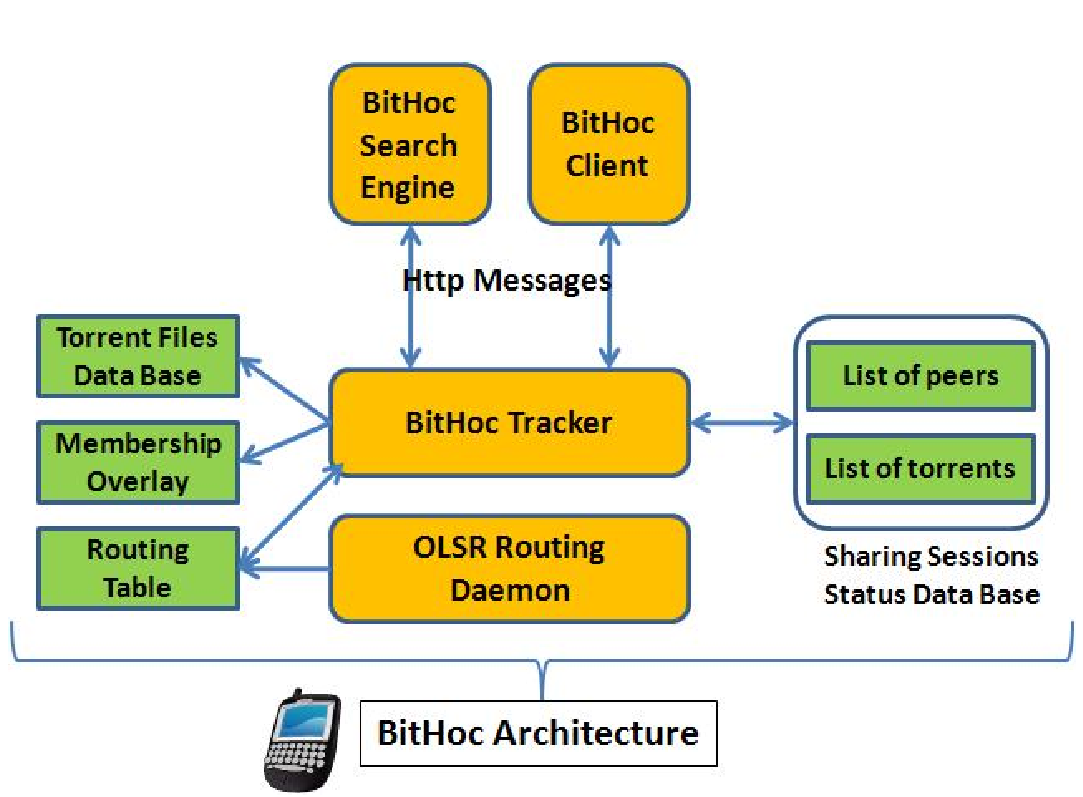
\includegraphics[width=0.7\textwidth]{Chapitre2/architecture.png}
  \end{center}
  \caption{Architecture of BitHoc}
  \label{figarch}
\end{figure}

\paragraph{Content publishing and discovery}

A user willing to share some content with the members of his community needs to indicate to the BitHoc client the location of the content in the mobile device file system. First, the client creates a meta-info file (Torrent file) that identifies in a unique manner a sharing session for this specific content. After that, the user publishes (locally) the new torrent file and a short text description of the related content using the BitHoc Search Engine service, which will update the local Torrent file database maintained in the underlying BitHoc Tacker via HTTP messages. A remote user, willing to share the same content, has to use the BitHoc search engine to find and download the Torrent file. He specifies for that the name of the content or some keywords related to its description. The request is sent via HTTP messages to its local tracker which looks for the closest match in its local database. If there are no matches, it forwards the HTTP request to the other trackers in the discovery overlay. Then, it presents the received results through an ergonomic user interface (see Figure \ref{Figsearchengine}). Based on the details of received answers (fitness to the search, number of peers involved in the sharing session, number of seeders, and number of lechers, etc), the user can choose the torrent file to download, then start sharing the content using the BitHoc Client.

\begin{figure}[!h]
  \begin{center}
    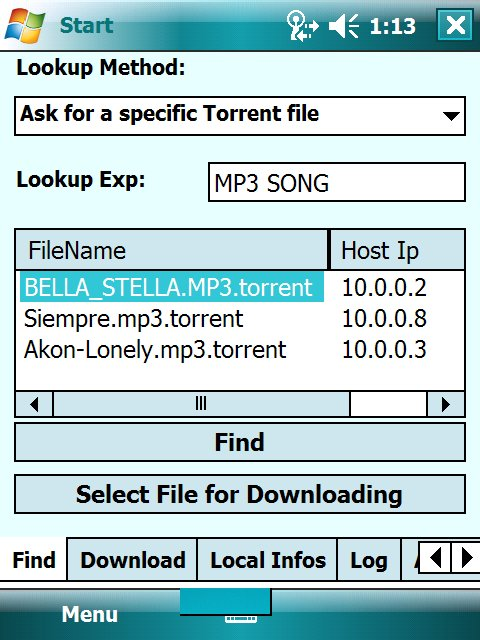
\includegraphics[width=2in,height=3in]{Chapitre2/searchengine.png}
  \end{center}
  \caption{Search Engine screen shot}
  \label{Figsearchengine}
\end{figure}

\paragraph{Membership management}

When a peer wants to join or leave the sharing session, the BitHoc client informs the BitHoc Tracker about this event using a specific HTTP message. This local agent disseminates this modification to the other BitHoc Tracker agents in other nodes in order to update their knowledge about the global membership information. The communications between Tracker agents are established in an event-driven fashion and use HTTP messages. Each tracker holds a HTTP server accepting HTTP requests from other agents and from the local BitTorrent client. The BitHoc Tracker component receives from the routing daemon up-to-date routing entries. In our testbed, the dynamics of the Ad-Hoc network are captured by the OLSR routing protocol \cite{OLSR}. Each time the number of hops toward a given peer changes, the routing daemon fires an event, which will be caught by the BitHoc Tracker and forwarded internally to the BitHoc client. This way we are sure the peer selection strategy always uses the updated number of hops to other peers. The parameters of the communications among tracker agents like HTTP listening ports and IP addresses can easily be configured by users via an ergonomic GUI. In addition to these functionalities, the BitHoc Tracker allows the user to monitor in real-time the status of the overlay (Contents it shares, members of the session, current topology of the Ad-Hoc network). He can even decide to keep traces about all the events in a file. For this, he just needs to activate the tracing option provided by the application.

\paragraph{Content sharing}

Before starting a new sharing session, the user can choose between two versions of BitTorrent algorithms: The classical version \cite{RefBT} and our version adapted to mobile Ad-Hoc networks described in~\cite{BitHoc}. The BitHoc client offers a Wizard allowing the user to configure the parameters of BitTorrent (communication ports, choking slot duration, minimum and maximum number of peers, etc). Once the torrent file is obtained, the BitHoc client can start the sharing session where it can either play the role of a leecher or a seed. It contacts periodically the local BitHoc tracker to get the current list of members of the same content sharing session (torrent). Using this list and the routing table, it manages the connections with the interested peers. Briefly a client implementing our algorithms exchanges pieces with close peers and only seeds distribute pieces across the network. Note that we allow the user to pause or resume the download while conserving the session context. He can also monitor in real time the status of the session (downloaded bytes, uploaded bytes, numbers of leechers, number of seeders, elapsed time, etc). Furthermore, the BitHoc client keeps in a log file statistics on the content sharing session and provides different levels of event traces. It also manages the storage of the downloaded contents and their classification. Figure \ref{Figclient} shows a screen-shot of the BitHoc client.

\begin{figure}[!h]
  \begin{center}
    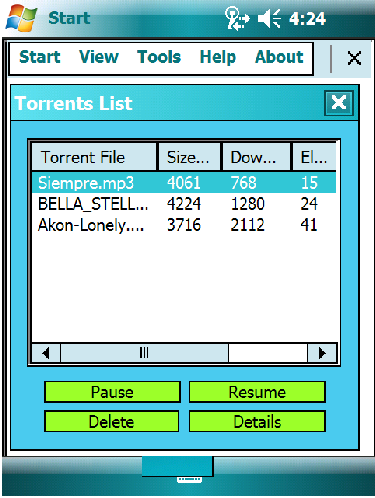
\includegraphics[width=2in,height=3in]{Chapitre2/contentsharing.png}
  \end{center}
  \caption{BitHoc Client screen shot}
  \label{Figclient}
\end{figure}

\subsubsection{Experimentation and results}
\label{sectest}

\paragraph{Test-bed description}

Our wireless Ad-Hoc network experimental environment consists of 14 mobile devices including 7 PDAs (HP iPAQ 214) and 7 smart-phones (HP iPAQ 614c). Each hand-held is equipped with an IEEE802.11b wireless card. The characteristics of the two types of devices are detailed in Table \ref{tabcarac}. The Ad-Hoc connectivity is maintained thanks to OLSR daemons run by the different devices. In our experiments, we constructed several network topologies containing a maximum of 6 hops. The objective of the realized swarm was to download a 4 MB MP-3 content. All PDAs were supposed to participate to the sharing of the file. The original seed of the content was chosen randomly among the set of the 14 PDAs.

\begin{table}[!h]
\center
\label{tabcarac}
\caption{Characteristics of mobile hand-held(s)}
\begin{tabular}{|l|c|c|}
  \hline
   & \textbf{PDA} & \textbf{Smart-phone} \\
  \hline
  \textbf{Name} & HP iPAQ 214 & HP iPAQ 614c\\
\hline
  \textbf{Processor speed} & 624 MHz & 520 MHz \\
  \hline
\textbf{RAM} & 128 MB & 128 MB \\
  \hline
\textbf{Operating system} & Windows Mobile 6 & Windows Mobile 6 \\
  \hline
\end{tabular}
\end{table}

\paragraph{Experimentation results}

\begin{figure}[!h]
  \begin{center}
    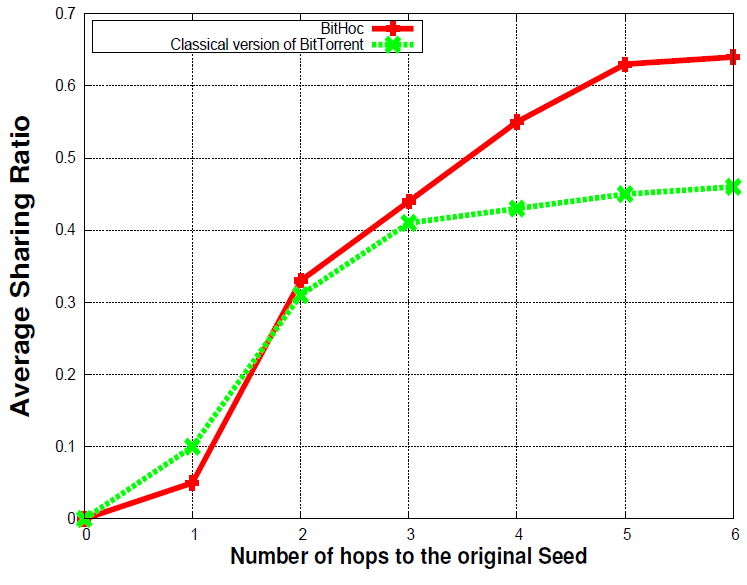
\includegraphics[width=3in,height=2.2in]{Chapitre2/sharingratio.png}
  \end{center}
  \caption{Sharing ratio}
  \label{figsharing}
\end{figure}

\begin{figure}[!h]
  \begin{center}
    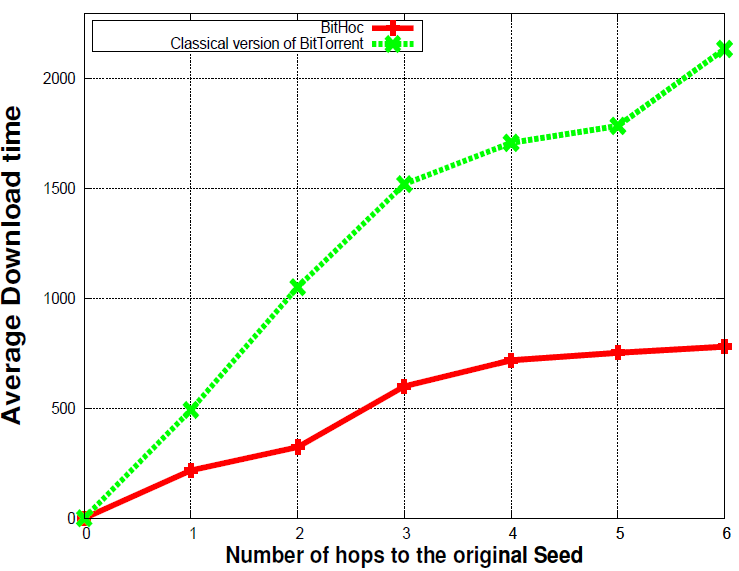
\includegraphics[width=3in,height=2.2in]{Chapitre2/downloadtime.png}
  \end{center}
  \caption{Download time}
  \label{FigDownloadtime}
\end{figure}

The metrics tracked during our experiments are the download time and the average sharing ratio of nodes. We define $R_{h}$ as the sharing ratio of peers located at $h$ hops from the original seed. It measures the level of reciprocity between downloads and uploads. In the ideal case, the ratio should be close to $1$. The two versions of BitTorrent (The legacy one and ours) have been tested and the results are presented in Figures \ref{figsharing} and \ref{FigDownloadtime}. Figure \ref{figsharing} shows a dramatic increase of sharing opportunities when our adapted version is deployed. The routing overhead generated by the classical version makes any gain obtained by important diversification of pieces negligible. Our method finds the good equilibrium between sharing and diversification. Figure \ref{FigDownloadtime} shows that BitHoc outperforms the classical version of BitTorrent in terms of download time. It is in accordance with our research results presented in~\cite{BitHocWeb}. More information about our experiments and our GPL licensed open-source code can be found on the BitHoc web site \cite{BitHocWeb}.

\subsubsection{BitHoc limitations with respect to a disruption prone environment}
\label{BitHoc:limitations}

We should note that BitHoc is built based on the assumptions that the network path are almost stable and that content providers and content consumers are connected to the same part of the network at the same time. Indeed, as described in Figure~\ref{figarch}, BitHoc relies on the routing table built and maintained by the OLSR MANET routing protocol towards maintaining the sharing sessions membership overlay and in order to deliver messages to peers at more than one hop. Therefore, BitHoc is not suitable solution for content dissemination in a disruption tolerant environment. 

\section{Content sharing in Disruption Tolerant Networks}

\subsection{Disruption Tolerant Networks}

Delay and disruption tolerant networks (DTNs) are a new class of wireless networks that seek to address the networking issues in mobile or challenging environments that lack
continuous network connectivity. DTNs have emerged recently and are continuing to gain extensive efforts from the networking research community~\cite{Bundle,fall03,dtnrg}. In the literature, these networks are found under different terminologies such as sparse mobile ad hoc networks, extreme wireless networks, or under another commonly used term intermittently connected networks. Basically, DTNs appear in areas where the network spans over large distances with low node density and/or with high node mobility. DTNs might appear also due to short radio range, power saving mechanism at the nodes, or nodes failure. Examples of such networking scenarios include, but are not limited to :

\begin{itemize}
\item{Vehicular networks, e.g.~\cite{Levine:MaxProp, DriveThru}. In~\cite{DriveThru}, the authors propose the Drive-thru Internet architecture where the objective is to provide network and Internet connectivity
to mobile users in vehicles. The network is constituted by hot spots that are placed along the roads providing thus intermittent connectivity to the users that can
connect within proximity. In~\cite{Levine:MaxProp}, Burgess et al. introduce UMass DieselNet which is a network made of 30 buses equipped with 802.11b wireless interfaces and GPS devices. The objective of the network is to provide real DTN testbed for experimental and research studies. The buses move on regular trajectories inside the UMass Amherst campus and surrounding areas. When two buses pass nearby, they transfer data to each other. Additionally, buses can connect to open wireless access points
along the roads.}
\item{Mobile sensor networks for environmental monitoring, e.g.~\cite{zebranet02,WirelessInfostation}. Zebranet~\cite{zebranet02} is a wireless networking architecture designed to support wildlife tracking for biology research. In ZebraNet, the network is constituted by sensor collars that are attached to zebras, which log movement patterns of the zebras, and by base stations that are mounted on cars which move around sporadically. When two zebras meet, the corresponding sensors exchange collected data for a potential data delivery back to base-stations. Another similar biological acquisition system has been proposed in~\cite{WirelessInfostation}, where the network is made of a set of sensors attached to whales and a set of fixed info-stations that act as collecting nodes.}
\item{Communication between rural zones in developing countries, e.g.~\cite{Brewer:DTNdeveloping}. Examples include DakNet~\cite{Brewer:DTNdeveloping} which is a wireless ad hoc network that has the capacity to provide asynchronous Internet access to remote rural residents using motorcycles and buses to carry users email and web search messages.}
\item{Deep space networks such as the Inter-planetary network (IPN)~\cite{interplanetary03}. The interplanetary network is a network of regional Internet networks. A region is an area where the characteristics of communication are the same. An example of regions includes the terrestrial Internet as a region or a ground-to-orbit region. IPN aims to achieve end-
to-end communication through multiple regions in a disconnected, variable-delay environments.}
\item{Challenged networks such as disaster healing networks after natural disaster, travel information and advertisements dissemination systems in large cities using local transport systems, military ad hoc networks where disconnection occurs because of the war or for security reasons where some links need to be shut down from time to time.}
\end{itemize}

Generally speaking, DTNs are wireless networks that do not conform to Internet or to traditional multi-hop and ad hoc wireless networks underlying structures and assumptions.
In particular, they are characterized mainly by the following specific features~\cite{fall03, DTNTutorial}:

\begin{itemize}
\item{Intermittent connectivity where an end-to-end path between a given source-destination pair does not exist most of the time. Path disconnections are frequent and arise from
two main factors, namely motion and/or limited power at the nodes. Disconnections due to motion can arise when one or both nodes at the end of a communication link move, or due to some intervening objects or signals that obstruct the communication. These disconnections can be predicted, for instance when the nodes move away
according to a predetermined schedule, or opportunistic for instance according to random walk of the nodes. Disconnections that are due to power outage result
commonly from some power saving mechanisms at the wireless devices, e.g. case of sensor networks. The latter disconnections are often predictable.}
\item{Nodes have low power capabilities and limited resources. In many DTNs, nodes are generally battery powered and/or deployed in areas lacking power infrastructure. In
some other situations, nodes have limited memory and/or processing capabilities.}
\item{Large delays which are basically due to long queuing times resulting from frequent disconnections, or from low data rate at the devices.}
\end{itemize}

\subsection{Content Sharing in Disruption Tolerant Networks}

Due to frequent disconnections in DTNs, instantaneous end-to-end routes do not exist, and hence most of the traditional Internet and/or mobile ad hoc content routing protocols fail~\cite{Fall:DTNrouting}. However, end-to-end routes may exist over time if the nodes can take advantage of their mobility by exchanging and carrying other nodes messages upon meetings, and by delivering them afterward to their corresponding destinations. The latter concept has given rise to a novel routing paradigm in these networks called the \emph{carry-and-forward approach}, in which intermediate nodes serve as relays for each other. Thus, the term "mobility-assisted routing approach" that is used in conjunction to describe these schemes.

Unfortunately, these techniques result in high latency, since packets need to be carried for long time periods before being delivered. When the delivery latency is not critical, as
the case of delay-tolerant networks, the store-carry-and-forward paradigm can prove to be adequate. For instance, this is the case when the delivery of the messages is very important, possibly more important than the delay. Basically, with the store-carry-and-forward approach, the delivery delays of packets depend on the rate at which contact opportunities are created in the network, as well as the availability of network resources, such as storage space and energy. The various studies that considered routing techniques in DTNs have examined the trade-offs between optimizing the delivery ratio and delivery delay from one side, and reducing nodes resources consumptions in terms of storage and battery usage from the other side. However, the intricacy of each one depends on the particularity of network environment at hand, the mobility model of the nodes, the performance objectives to attain, and other criteria.

This section will survey and classify various research works that have considered content routing schemes for DTNs. Actually, there are different approaches to categorize these schemes~\cite{Ward:RoutingSurvey, DTNRoutingSurvey06}. Hereafter, we propose a classification that is based on the content distribution method. Specifically, depending on whether these schema operate on a point-to-point basis or point-to-multipoint one.

\subsubsection{Point to Point Content Routing in Disruption Tolerant Networks}

We classify existing DTN point-to-point routing protocols as those that replicate packets and those that forward only a
single copy. Epidemic routing protocols replicate packets at transfer opportunities hoping to find a path to the destination.
However, naive flooding wastes resources and can severely degrade performance. Proposed protocols attempt to limit
replication or otherwise clear useless packets in various ways: \emph{(i)} using historic meeting information~\cite{Wearable, MVRouting, Levine:MaxProp}; \emph{(ii)} removing useless packets using acknowledgments of delivered data~\cite{Levine:MaxProp}; \emph{(iii)} using probabilistic mobility information to infer
delivery~\cite{Haas:wdtn}; \emph{(iv)} replicating packets with a small probability~\cite{Tseng:broadcast}; \emph{(v)} using network coding~\cite{LeBoudec:wdtn} and coding with
redundancy~\cite{Fall:Sigcomm05}; and \emph{(vi)} bounding the number of replicas of a packet~\cite{Haas:wdtn,akis:wdtn,Vahdat:epidemic}.

In contrast, forwarding routing protocols maintain at most one copy of a packet in the network~\cite{Fall:DTNrouting,Waterloo:wdtn,akis:technical1}. Jain et
al.~\cite{Fall:DTNrouting} propose a forwarding algorithm to minimize the average delay of packet delivery using oracles with varying
degrees of future knowledge. Deployment experience~\cite{BalasubramanianLV07} suggests that, even for a scheduled bus service, implementing
the simplest oracle is difficult; connection opportunities are affected by many factors in practice including weather, radio
interference, and system failure. Jones et al.~\cite{Waterloo:wdtn} propose a link-state protocol based on
epidemic propagation to disseminate global knowledge, but use a single path to forward a packet. Shah et al.~\cite{Shah:datamules} and
Spyropoulos et al.~\cite{akis:technical1} present an analytical framework for
the forwarding-only case assuming a grid-based mobility model. They subsequently extend the model and propose a
replication-based protocol, Spray and Wait~\cite{akis:wdtn}. The consensus~\cite{akis:wdtn} appears to be that replicating packets can improve
performance (or security~\cite{Levine:Mobihoc07}) over just forwarding, but can risk degrading performance when resources are limited.

Our position is that most existing point-to-point routing schemes does not take into consideration the impact of buffer management and scheduling policies on the performance of the underlaying system. The later issues has been largely disregarded, in comparison, by the DTN community. And thus, most routing protocols only have an incidental effect on desired performance metrics, including commonly evaluated metrics like average delay or delivery probability. For example, Spray and Wait~\cite{akis:wdtn} like many other routing protocols~\cite{Haas:wdtn,Vahdat:epidemic} that route packets using the number of replicas as the heuristic to enhance a given routing metric, does not take explicitly into account bandwidth or storage constraints which makes the effect of their design decision on the performance of a given resource constrained network scenario unclear. Nevertheless, some works already investigated the impact of plugging simple drop policies to already existing routing protocols in~\cite{Towsley:Epidemic}, Zhang et al. present an analysis of buffer constrained \emph{Epidemic} routing, and evaluate some simple drop policies like drop-front and drop-tail. The authors conclude that drop-front, and a variant of it giving priority to source messages, outperform drop-tail in the DTN context. A somewhat more extensive set of combinations of \emph{heuristic} buffer management policies and routing protocols for DTNs is evaluated in~\cite{QueuingPolicies}, confirming the performance of drop-front. In~\cite{DCopies}, Dohyung et al. present a drop policy which discards a message with the largest expected number of copies first to minimize the impact of message drop. However, all these policies are also heuristics, i.e. not explicitly designed for optimality in the DTN context. Also, these works do not address scheduling. 

Yet, the combination of long-term storage and the, often expensive, message replication performed by many DTN routing protocols impose a high bandwidth and storage overhead on wireless nodes. Moreover, the data units disseminated in this context, called bundles, are self contained, application-level data units, which can often be large. As a result, it is expected that nodes' buffers, in this context, will often operate at full capacity. Similarly, the available bandwidth during a contact could be insufficient to communicate all intended messages. Consequently, we believe that regardless of the specific routing algorithm used, it is important to have: \emph{(i)} efficient drop policies to decide which content(s) should be discarded when a node's buffer is full, and \emph{(ii)} efficient scheduling policies to decide which content(s) should be chosen to exchange with another encountered node when bandwidth is limited. 
\begin{table}[!h]
\renewcommand{\arraystretch}{1.1}
\caption{A classification of some related work into DTN routing scenarios}
\centering
\footnotesize
\begin{tabular}{|p{1cm}|p{1.5cm}|p{1.7cm}|p{1.5cm}|p{5cm}|}
\hline
\bfseries Cat. &\bfseries Storage &\bfseries Bandwidth  &\bfseries Routing& \bfseries Work (and mobility)\\
\hline
\bfseries R1&Unlimited & Unlimited &Replication & Epidemic~\cite{Vahdat:epidemic}, Spray and Wait~\cite{akis:wdtn}: Constraint in the form of
channel contention (Grid-based synthetic)\\
\hline
\bfseries R2&Unlimited & Unlimited &Forwarding & Modified Djikstra's algorithm Jain et al.~\cite{Fall:DTNrouting} (simple graph),
MobySpace~\cite{DTNSpace} (Powerlaw)\\
\hline
\bfseries R3&Finite & Unlimited &Replication &Davis et al.~\cite{Wearable} (Simple partitioning synthetic), SWIM~\cite{Haas:wdtn} (Ex-
ponential), MV~\cite{MVRouting}(Community-based synthetic), Prophet~\cite{prophet03}
(Community-based synthetic) \\
\hline
\bfseries R4&Finite & Finite & Forwarding& Jones et al.~\cite{Waterloo:wdtn} (AP traces), Jain et al.~\cite{Fall:DTNrouting} (Synthetic DTN topol-
ogy)\\
\hline
\bfseries R5&Finite & Finite &Replication & Our proposal (Vehicular DTN traces, testbed deployment), RAPID~\cite{Levine:Sigcomm07} (Vehicular DTN traces, testbed deployment), MaxProp~\cite{Levine:MaxProp} (Vehicular DTN traces) \\
\hline
\end{tabular}
\label{RoutingSummary}
\end{table}

Table~\ref{RoutingSummary} shows a taxonomy of many existing DTN routing protocols based on assumptions about available bandwidth during transfer opportunities and the storage
capacity carried by wireless nodes; both are either finite or unlimited. For each work, we state in parentheses the mobility model used. 
Categories $R1$ and $R2$~\ref{RoutingSummary} are important to examine for valuable insights that theoretical tractability yields but are impractical for real DTNs with limited resources. Many studies~\cite{Lindgren:probabilistic,Wearable,MVRouting} analyze the case where storage at nodes is limited, but bandwidth is unlimited ($R3$). This scenario may happen when the radios used and the duration of contacts allow
transmission of more data than can be stored by the nodes. However, we found this scenario to be uncommon typically because storage is inexpensive and energy efficient. Trends suggest that high bit rate radios will remain more expensive and energy-intensive than storage~\cite{PRESTO}. Finally, for mobile DTNs, and especially vehicular DTNs, transfer opportunities are short-lived~\cite{Levine:MaxProp}.

We were able to find mainly two protocols that belong to the category $R5$. The first, Max-Prop~\cite{Levine:MaxProp}, assumes limited storage and bandwidth. However, it is unclear how to optimize a specific routing metric using MaxProp, so we categorize it as an incidental routing protocol. And the second, RAPID~\cite{BalasubramanianLV07}, is the first protocol to explicitly assume both bandwidth and (to a lesser extent) buffer constraints exist, and to handle the DTN routing problem as an optimal resource allocation problem, given some assumption regarding node mobility. As such, it is the most related to our work, and we will compare  directly against it. Despite the elegance of the approach, and performance benefits demonstrated compared to well-known routing protocols, RAPID suffers mainly from the following drawbacks: \emph{(i)} its policy is based on suboptimal message utilities (more on this in Section~\ref{sec:optimal-policy}); \emph{(ii)} in order to derive these utilities, RAPID requires the flooding of information about all the replicas of a given message in the queues of all nodes in the network; yet, the information propagated across the network might arrive stale to nodes (a problem that the authors also note) due to change in the number of replicas, change in the number of messages and nodes, or if the message is delivered but acknowledgements have not yet propagated in the network; and \emph{(iii)} RAPID does not address the issue of signaling overhead. Indeed, in~\cite{Levine:Sigcomm07}, the authors showed that whenever the congested level of the network starts increasing, their meta-data channel consumes more bandwidth. This is rather undesirable, as meta-data exchange can start interfering with data transmissions amplifying the effects of congestion. In another work~\cite{AOBM}, Yong et al. present a buffer management schema similar to RAPID. However they do not address the scheduling issue nor the trade-off between the control channel overhead and system performance. Through our proposal to be described in Chapters~\ref{chapter:ptp} and~\ref{chapter:HBSD}, we successfully address all these three issues.

\subsubsection{Point to Multi-Point Content Dissemination in Disruption Tolerant Networks}

As highlighted in the latter section, a significant share of research on opportunistic networks has focused on \emph{unicast} point-to-point content routing (see e.g.~\cite{DTNTaxonomy} or~\cite{Passarella:Survey}). Instead, in a second part of this dissertation, we consider the problem of content dissemination. This is a key research problem, 
particularly in opportunistic networks. In this environment, according to the user-generated content wave, users are expected to generate large amounts of content 
by exploiting capability-rich mobile devices (such as PDAs, smart-phones, etc.), and to share them with people around them.  The problem of efficiently disseminating contents in opportunistic networks is thus very relevant, and not widely explored in the literature yet.
 
Content dissemination in opportunistic networks is a difficult problem. As the topology is very unstable, and users appear and disappear from the network dynamically, content providers and content consumers might be completely unaware of each other, and never connected at the same 
time to the same part of the network. Therefore, contents should be moved and replicated in the network in order to carry them to interested users despite disconnections 
and partitions. On the other hand, content dissemination systems should take care of both network and device resource constraints.
For example, a trivial solution would be to flood the whole network with any generated content, but this would clearly saturate both network resources (in terms of available bandwidth) and device resources (e.g., in terms of energy, storage, etc.). Content dissemination systems should also take care of the willingness of people to collaborate. Indeed,  
experience teaches us that selfish behavior is often the norm, unless incentives are provided, and can be a major impediment to any such peer-to-peer system in the wild~\cite{NashEquilibria}. Thus, we believe that content dissemination systems should consider users to be inherently selfish, instead of inherently collaborative, and provide the necessary mechanisms to enforce collaboration and prevent the bad impact of selfish behaviors on the overall system performance.  

Content dissemination systems have been proposed for the Internet, and also for conventional MANETs~\cite{BitHoc}. In general, these systems assume that network paths are rather stable, and often generate a significant amount of traffic to maintain knowledge of other devices' caches. Therefore, they are not suitable for opportunistic networks. Table~\ref{DisseminationSummary} shows a taxonomy of most of existing DTN content dissemination systems. We classify the later systems into three categories, namely  
\emph{D1} content centric dissemination systems guided by users \emph{Interests}, \emph{D2} systems driven by users interests + social links and finally
\emph{D3}, dissemination systems guided by users interests and their locations. We also detail in Table~\ref{DisseminationSummary} whether the presented content dissemination systems provide or not needed mechanisms to handle devices' buffers management in case of congestion, contents scheduling during short lived contact opportunities and users selfishness. 

\begin{table}[!h]
\renewcommand{\arraystretch}{1.1}
\caption{A classification of content dissemination systems for DTN(s)}
\centering
\footnotesize
\begin{tabular}{|p{1cm}|p{2cm}|p{9.5cm}|}
\hline
\bfseries Cat. &\bfseries Driven by&\bfseries Work (buffer management, scheduling, users selfishness, mobility)\\
\hline
\bfseries D1&Users Interests & Our proposal, MobiTrade(handled, handled, inherently selfish, Vehicular DTN traces \& testbed deployment), DTN Podcasting by May et al.~\cite{May07wirelessopportunistic}~\cite{Lenders:Podcast}(not handled, not handled, inherently collaborative, testbed deployment), TACO-DTN by Solazzo et al.~\cite{TACODTN}(handled, handled, inherently collaborative, random waypoint), \\
\hline
\bfseries D2&Users Interests + Social Links &ContentPlace by Boldrini et al.~\cite{Chiara:MSWIM08}(handled, handled, inherently collaborative, synthetic based on the HCMM model~\cite{HCMM}), SocialCast by Helgason et al.~\cite{SocialCast2, SocialCast}(not handled, not handled, inherently collaborative, real human mobility traces + testbed deployment)\\
\hline
\bfseries D3&Users Interests + Location & Locus by Thompson et al.~\cite{LOCUS}(handled, handled, inherently collaborative, synthetic via MobiSim~\cite{MobiSim}), PeopleNet by Motani et al.~\cite{Peoplenet}(handled, not handled,inherently collaborative, random walk)\\
\hline
\end{tabular}
\label{DisseminationSummary}
\end{table}

TACO-DTN~\cite{TACODTN} by Sollazzo et al. is a time-aware approach to delay tolerant content based dissemination. It is implemented as a publish/subscribe system and is mainly designed to distribute temporal events to subscribed users. TACO-DTN supposes that a number of nodes act as \emph{infostations}, enjoying some form of connectivity to the backbone, and other nodes are mobile devices, reachable sometimes only through intermittent connectivity of carriers. Examples of applications benefiting from such a system could be travel information dissemination systems in  large cities (exploiting info-stations at bus stops) or on highways, advertisements dissemination at specific times, and information dissemination to remote villages. In TACO-DTN, temporal profiles are associated to each subscription and allow the construction of temporal profiles of \emph{info-stations}. Events also have temporal validity. TACO-DTN uses temporal profiles in order to achieve two main tasks: \emph{(i)} buffer management, in order to decide which events to store when buffer space is limited, and \emph{(ii)} event routing, to select the right info-station or carrier on which to publish content. While TACO-DTN is a content/event dissemination system that handle both events routing as well as info-stations' buffers management, it does not provide an optimal dissemination schema that maximizes the collaborative end users satisfaction and prevent selfish ones from impairing the temporal events dissemination process.

In~\cite{Peoplenet}, authors claim that people often use social contacts for time, location and community-specific information rather than using powerful search engines or libraries and that social contacts are generally good sources of this information. Then, authors propose  \emph{PeopleNet}~\cite{Peoplenet} as a simple and efficient mechanism to find location, time, and community-specific information between people. PeopleNet is a query matching system that exploits the: natural behaviors of social networking and social mobility, together with the pervasiveness of mobile phones and their P2P capabilities. Indeed, Peoplenet~\cite{Peoplenet} is hybrid system that propagates and matches queries over, first, infrastructure, and second, using DTN device-to-device communication in the wireless "last hop" (e.g. inside a cell) to forward further. It uses the  infrastructure to propagate queries of a given type to users in specific geographic locations, called \emph{bazaars}. Within each bazaar, the query is further propagated between neighboring nodes via peer to peer connectivity until it finds a matching query. While authors provide a set of heuristics to manage content scheduling and forwarding upon an opportunistic meeting between two mobile nodes, they do not provide optimal buffer management policies in case of nodes buffers congestion. Through PeopleNet~\cite{Peoplenet}, authors also suppose that wireless mobile nodes are inherently collaborative and hence, do not address users selfishness problem. Indeed, in such a context, experience teaches us that selfish behavior is often the norm, unless incentives are provided, and can be a major impediment to any such peer to peer system~\cite{NashEquilibria}.
  
BlueTorrent~\cite{BlueTorrent} is an opportunistic file sharing application for Bluetooth enabled devices that mimics BitTorent~\cite{RefBT}. Authors propose an index (shared contents database) dissemination and file swarming protocols for dynamic, sparse networks. The concept of distributing large files using small atomic chunks is similar to our proposal. However, BlueTorrent relies on Bluetooth whereas our proposal leverages any link-layer technologies. Furthermore, unlike BlueTorrent, we propose to structure the data in the network into channels and rely instead on an entirely receiver-driven content dissemination protocol. Instead, BlueTorrent mimics BitTorent for both contents and peers management. Indeed, it relies on a heavy content management block that maintains a bitmap matrix for each content to track downloaded and missed pieces, this bitmap matrix is later exchanged between peers. It also relies on a heavy peers management block that should keep track of encountered peers and their collaboration level in order to be able to select the best peers among neighboring devices.

SocialCast~\cite{SocialCast2, SocialCast} is an interest driven content distribution framework that complements the information about the receivers' interests, necessary to routing information, with data about the social ties of people and their consequent predicted movements. In SocialCast, Kalman filter forecasting techniques, are used to predict the future evolution of the movement based on previous observations on some attributes characterizing social behavior. These predictions are used to derive an utility $U_i$ per device and interest/channel \emph{i}, the latter utility is used to identify whether the corresponding device is the best carrier for the contents matching
the interest \emph{i} or not with respect to all the neighbors devices. Compared to SocialCast, our solution does not rely on any self-declared social information/ties and MobiTrade uses a considerably more sophisticated utility that tracks users physical detected social links and considers both content demand/popularity as well as the collaboration level of the encountered peers (in order to re-act to selfish behaviors).

In~\cite{Boldrini:2008:MDD}, Boldrini et al. present also a content centric approach for DTNs. Authors propose a utility-based cooperative data dissemination system in which the utility of data is defined based on the social
relationships (physical detected ones) between users.  The main idea is that nodes gather other users' interests during contacts, and estimate the availability of the corresponding data objects in the network. They use this information to compute utility values for data objects (channels) they "see" (i.e., objects that are available on encountered nodes), and to decide what to fetch and store locally. This decision is also based on the cost of the data objects in terms of resource consumption (energy, ...). They further consider that users are inherently collaborative.

To our best knowledge, the only other work looking at pure content centric dissemination architecture for opportunistic networks is the research thread first initiated by the PodNet project~\cite{May07wirelessopportunistic, podnet07}. This work proposes a DTN Podcasting architecture, built around the concept of \emph{content channels}, that we also use in our work. In the first version of PodNet~\cite{May07wirelessopportunistic}, users only store and share channels they are interested in. So, there is no content forwarding. In a later version~\cite{podnet07}, simple strategies to cache other \emph{foreign} channels as well are considered, in order to force content forwarding and  improve the overall system performance. 
 
ContentPlace~\cite{ContentPlace} by Boldrini et al. attempts to improve Podcasting using explicit knowledge of social networking links of participants. The idea behind ContentPlace is to exploit social information on the environment the nodes operate, in order to enhance content dissemination. In the framework of opportunistic networks, this approach has already been successfully applied to message forwarding (e.g., \cite{Boldrini:SocialForwarding}). The idea is to
move messages closer and closer to their destinations following a path based on the social interactions between nodes. In the case of forwarding protocols, however, messages have a specific destination node, while in ContentPlace, following the user generated content 
approach, content generators might be unaware of the nodes interested in their data, and so might be the content consumers about the
nodes that generate the content they are interested in. ContentPlace provides also mechanisms to handle devices' buffers congestion and content scheduling. Indeed, it assumes that users belong to social communities, and learns in an autonomous way the time
spent by them in each community, which types of contents users of each community are interested in, and how
spread in the communities the contents are. This information is used to evaluate the utility of each encountered
content which is later used to evaluate the contents the remote peer is carrying and to select the ones that should be fetched in order to maximize the total utility of the 
contents in the local buffer. Compared to ContentPlace, MobiTrade does not require such user reported social information and does not make any hard assumptions regarding node mobility. 
 
Finally, the most recent work in this thread, by Hu et al~\cite{OptimalChannelChoice}, attempts a rigorous formulation of the problem of optimally matching channels (to store) to a population of devices. A distributed algorithm is then proposed based on the framework of Markov Chain Monte Carlo optimization. While we find this framework particularly interesting, it also comes at the expense of high complexity, long convergence delays (known in MCMC), and a need for carefully tuned simulated annealing~\cite{mcmc-bremaud}.

A major difference of our proposal (MobiTrade), is that we consider users to be inherently selfish, instead of inherently collaborative as in all the aforementioned studies. Experience teaches us that selfish behavior is often the norm, unless incentives are provided, and can be a major impediment to any such peer-to-peer system in the wild~\cite{NashEquilibria}. The only proposal we are aware of, dealing with selfish users in the context of DTNs is~\cite{BarterDTN}, where a Tit-For-Tat mechanism (''bartering'') is also used between nodes to exchange content. While Tit-For-Tat (TFT) ensures selfish users are blocked, it does not answer itself \emph{how collaborative nodes should optimally (re-)act in the presence of TFT}. This is answered in MobiTrade by a personalized inventory management mechanism, key to almost all the system's functions and good performance.

Note that many incentive approaches have been proposed in order to prevent selfish users from impairing point to point content routing protocols in the context of a delay tolerant network. However, as described in Table~\ref{DisseminationSummary}, almost all point-to-multipoint content dissemination systems in the literature do not considered this problem and suppose that users are inherently collaborative.

As a snapshot of the incentive approaches provided to support point to multi-point DTN routing systems we, cite:
\begin{enumerate}

\item In MoB~\cite{MoB}, authors propose an infrastructure for collaborative wide-area wireless data services that is supposed to provide access to the Internet (either through WLANs or cellular data networks). Towards that,  MoB proposes to decouple infrastructure providers from services providers and enables wireless services trading and sharing among interested users. MoB is also based on third-party centralized tools for accounting and billing as well as for reputation and trust management. Indeed, in order to enable such a services market, MoB requires \emph{(i)} a reputation and trust management system, and \emph{(ii)} a billing and accounting system, both of which can ideally be implemented by independent providers as third-party services. MoB uses Vito as a reputation management and accounting system. The design of the latter system is modeled on eBay. Compared to MobiTrade, MoB focus on services availability rather than content sharing and hence it does not provide any detailed architecture for optimal content sharing in the context of a DTN that can both deal with rational, selfish nodes.

\item Through MobiCent~\cite{MobiCent}, authors provide a credit-based system to support Internet access service in a heterogeneous wireless network environment. The considered case study scenario is the following: a mobile device is capable of operating in two modes. It can use a long-range low-bandwidth radio to maintain an always-on connection while using a short-range and high-bandwidth link (e.g.,Wi-Fi) to opportunistically exchange large amount of data with peers in its vicinity. Then, authors
claim that by default mobile devices are managed by autonomous and selfish parties, an hence propose an incentive scheme to foster cooperation among participants in the DTN. The proposed credit based system is supposed to work on top of any point-to-point DTN routing protocol. So, in two words, MobiCent makes the underlying point-to-point DTN routing protocol incentive compatible. 

\item The work \emph{Incentive-Aware Routing in DTNs}~\cite{IADTN} is very similar to MobiCent. Here also, authors suppose that DTN users are inherently selfish, therefore it is necessary to design incentive-aware routing for DTNs in order to fully take advantage of temporary connections. The proposed routing protocol is point-to-point. And authors simply introduce an LP formulation including TFT constraints in order to optimize the overall average delivery rate in a DTN. And in order to overcome respectively the bootstrapping issue and the possible lengthy retaliation between two neighbors, authors made propose to upgrade the TFT constraints within the LP formulation by making them account also for a generosity (enable initial cooperation of up to X) and contrition. This work as well as MobiCent are proposals to deal with selfish users within a DTN environment while considering an underlying point-to-point routing protocol. And these 
proposals does not have anything to do with point to multi-point content dissemination nor content centric architectures.

\end{enumerate}

As a final note, MobiTrade is not a reputation system, as e.g.~\cite{Reputation}. In reputation systems, nodes collect and share their opinions about peers with others. In our case, each device forms a personal opinion of peers used to only optimize her actions. Our system is more similar to a \emph{market} of independent traders. As a result, a bad customer for device $X$ might be a good customer for device $Y$.

\section{Conclusions and open issues}

In this chapter, we describe the background behind our work and we present the main solutions proposed in the literature for content routing in a disruption tolerant environment (both point-to-point content routing and point-to-multipoint routing protocols). However, as described in this chapter, despite the large amount of effort invested in the design of efficient point-to-point content routing protocols for DTN, there has not been a similar focus on storage management and scheduling policies. Indeed, we believe that regardless of the specific routing algorithm used, it is important to have: \emph{(i)} efficient drop policies to decide which content(s) should be discarded when a node's buffer is full, and \emph{(ii)} efficient scheduling policies to decide which content(s) should be chosen to exchange with another encountered node when bandwidth is limited. We describe later in Chapter~\ref{chapter:ptp}, the performance gain that the latter policies can engender if they are optimally designed. 

Furthermore, the point-to-multipoint content dissemination solutions described in this chapter does not provide an optimal dissemination schema that maximizes the collaborative end users satisfaction and prevent selfish ones from empairing the content dissemination process. To achieve the latter goals, we propose MobiTrade in Chapter~\ref{chapter:PTMP} as a candidate architecture. MobiTrade is a utility driven trading system for efficient content sharing on top of a DTN. It does not only take care of the network and device resources, but also carefully considers: the propagation of interests of participating users, the matching of these interests to individual node mobility patterns, and the willingness of involved users to collaborate.

In the remainder of this thesis, we start by studying the case of point-to-point content routing within a disruption tolerant network in Chapter~\ref{chapter:ptp} and we describe the greedy optimal solution that we propose. Then, we detail in Chapter~\ref{chapter:HBSD} the implementation issues of the latter solution. In Chapter~\ref{chapter:PTMP}, we present MobiTrade, our point-to-multipoint interest driven content sharing architecture for DTN. Then, we provide in Chapter~\ref{chapter:MobiTrade} a detailed implementation analysis of MobiTrade for smart-phones equipped with the Android platform.



\chapter{A Greedy Optimal Point-to-Point Content Routing Schema for DTN}
\label{chapter:ptp}
\minitoc

\section{Optimal Joint Scheduling and Drop Policy}
\label{sec:optimal-policy}

In this section, we first describe our problem setting and the assumptions for our theoretical framework. We then use this framework to identify the optimal policy, GBSD (Global Knowledge based Scheduling and Drop). This policy uses global knowledge about the state of each message in the network (number of replicas). Hence, it is difficult to implement it in a real world scenario, and will only serve as reference. In the next section, we will propose a distributed algorithm that can successfully approximate the performance of the optimal policy.

\subsection{Assumptions and Problem Description}
\label{subsec:ProblemDescription}

We assume there are $L$ total nodes in the network. Each of these nodes has a buffer, in which it can store up to $B$ messages in transit, either messages belonging to other nodes or messages generated by itself. Each message has a Time-To-Live ($TTL$) value, after which the message is no more useful to the application and should be dropped by its source and all intermediate nodes. The message can also be dropped when a notification of delivery is received, or if an ''anti-packet'' mechanism is implemented~\cite{Towsley:Epidemic}.

\textbf{Routing:} Each message has a single destination (unicast) and is assumed to be routed using a replication-based scheme~\cite{akis:ton-multi}. During a contact, the routing scheme used will create a list of messages to be replicated among the ones currently in the buffer. Thus, different routing schemes might choose different messages. For example, epidemic routing will replicate all messages not already present in the encountered node's buffer~\cite{Vahdat:epidemic}. For the purposes of this paper, we will use epidemic routing as a case study, for the following reasons. First, its simplicity allows us to concentrate on the problem of resource allocation, which is the focus of this paper. Second, it consumes the most resources per message compared to any other scheme. As a result, it can be easily driven to medium or high congestion regimes, where the efficient resource allocation problem is most critical. Third, given the nature of random forwarding schemes, unless a buffer is found full or contact capacity is not enough to transfer all messages, epidemic forwarding is optimal in terms of delay and delivery probability. Consequently, epidemic routing along with appropriate scheduling and message drop policies, can be viewed as a new routing scheme that optimally adapts to available resources~\cite{Levine:Sigcomm07}. Finally, we note that our framework could be used to treat other types of traffic (e.g. multicast), as well. %However, we focus on unicast traffic to elucidate the basic ideas behind our approach, and defer the treatment of multi-point traffic to future work.

\textbf{Mobility Model:} Another important element in our analytical framework is the impact of mobility. In the DTN context, message transmissions occur only when nodes encounter each other. Thus, \emph{the time elapsed between node meetings is the basic delay component}. The meeting time
distribution is a basic property of the mobility model
assumed~\cite{akis:mobihoc06,Inria:MessageDelay}\footnote{By \emph{meeting time} we refer to the time until two nodes starting from the stationary distribution come within range (''first meeting-time''). If some of the nodes in the network are static, then one needs to use \emph{hitting times} between mobile and static nodes. Our theory can be easily
modified to account for static nodes by considering, for example, two classes of nodes with different meeting rates (see e.g.~\cite{akis09}).}. To formulate the optimal policy problem, we will first assume a class of mobility models that has the following properties:
\begin{enumerate}
\item [A.1] Meeting times are exponentially distributed or have at least an \emph{exponential tail};
\item [A.2] Nodes move \emph{independently} of each other;
\item [A.3] Mobility is homogeneous, that is, all node pairs have the same meeting rate $\lambda$.
\end{enumerate}

Regarding, the first assumption, it has been shown that many simple synthetic mobility models like Random Walk, Random Waypoint and Random Direction~\cite{akis:mobihoc06,Inria:MessageDelay} have such a property. Furthermore, it is a known result in the theory of random walks on graphs that hitting times on subsets of vertices usually have an exponential tail~\cite{Aldous:book}. Finally, it has recently been argued that meeting and inter-meeting times observed in many traces also exhibit an exponential tail~\cite{LeBoudec:Mobicom07}. As we will see in Section~\ref{subsec:MaxAvgDeliveryRate}, in our framework, \emph{we sample the remaining meeting time only when a drop or scheduling decision needs to be taken}. In a sparse network (as in our case), it can be shown that, at this time, the two nodes in question have already \emph{mixed} with high probability. Thus, the quantity sampled can be approximated by the meeting time from stationarity, or the tail of the inter-meeting time distribution, which, as explained, is often exponential~\cite{Akis:IJAACS2008}. In other words, it is not required to make the stronger assumption of Poisson distributed inter-meeting times, as often done in related literature.

Regarding the second assumption, although it might not always hold in some scenarios, it turns out to be a useful approximation. In fact, one could use a mean-field analysis argument to show that independence is not required, in the limit of large number of nodes, for the analytical formulas derived to hold (see e.g.~\cite{LeBoudec:Sigmetrics09}).

Finally, in Section~\ref{section:heterogeneous-mobility}, we discuss how to remove assumption [A.3] and generalize our framework to heterogenous mobility models.

\textbf{Buffer Management and Scheduling:} Let us consider a time instant when a new contact occurs between nodes $i$ and $j$. The following resource allocation problem arises when nodes are confronted with limited resources (i.e. contact bandwidth and buffer space)\footnote{We note that, by ''limited resources'', we do not imply that our focus is only small, resource-limited nodes (e.g. wireless sensors), but rather that the offered forwarding or storage load exceeds the available capacity. In other words, we are interested in congestion regimes.}.

(\emph{Scheduling Problem}) If $i$ has $X$ messages in its \emph{local} buffer that it should forward to $j$ (chosen by the routing algorithm), but does not know if the contact will last long enough to forward all messages, which ones should it send first, so as to maximize the \emph{global} delivery probability for \emph{all} messages currently in the network?

(\emph{Buffer Management Problem}) If one (or more) of these messages arrive at $j$'s buffer and find it full, what is the best message $j$ should drop among the ones already in its buffer (\emph{locally}) and the newly arrived one, in order to maximize, let's say, the average delivery rate among all messages in the network (\emph{globally})?

To address these two questions, we propose the following policy. Given a routing metric to optimize, \emph{our policy, GBSD, derives a per-message utility that captures the \emph{marginal value} of a given message copy, with respect to the chosen optimization metric}. Based on this utility, two main functions are performed:

\begin{enumerate}
\item \emph{Scheduling}: at each contact, a node should replicate messages in decreasing order of their utilities.
\item \emph{Drop}: when a new message arrives at a node with a full buffer, this node should drop the message with the smallest utility among the one just received and the buffered messages.
\end{enumerate}

\begin{figure}[!h]
\centering
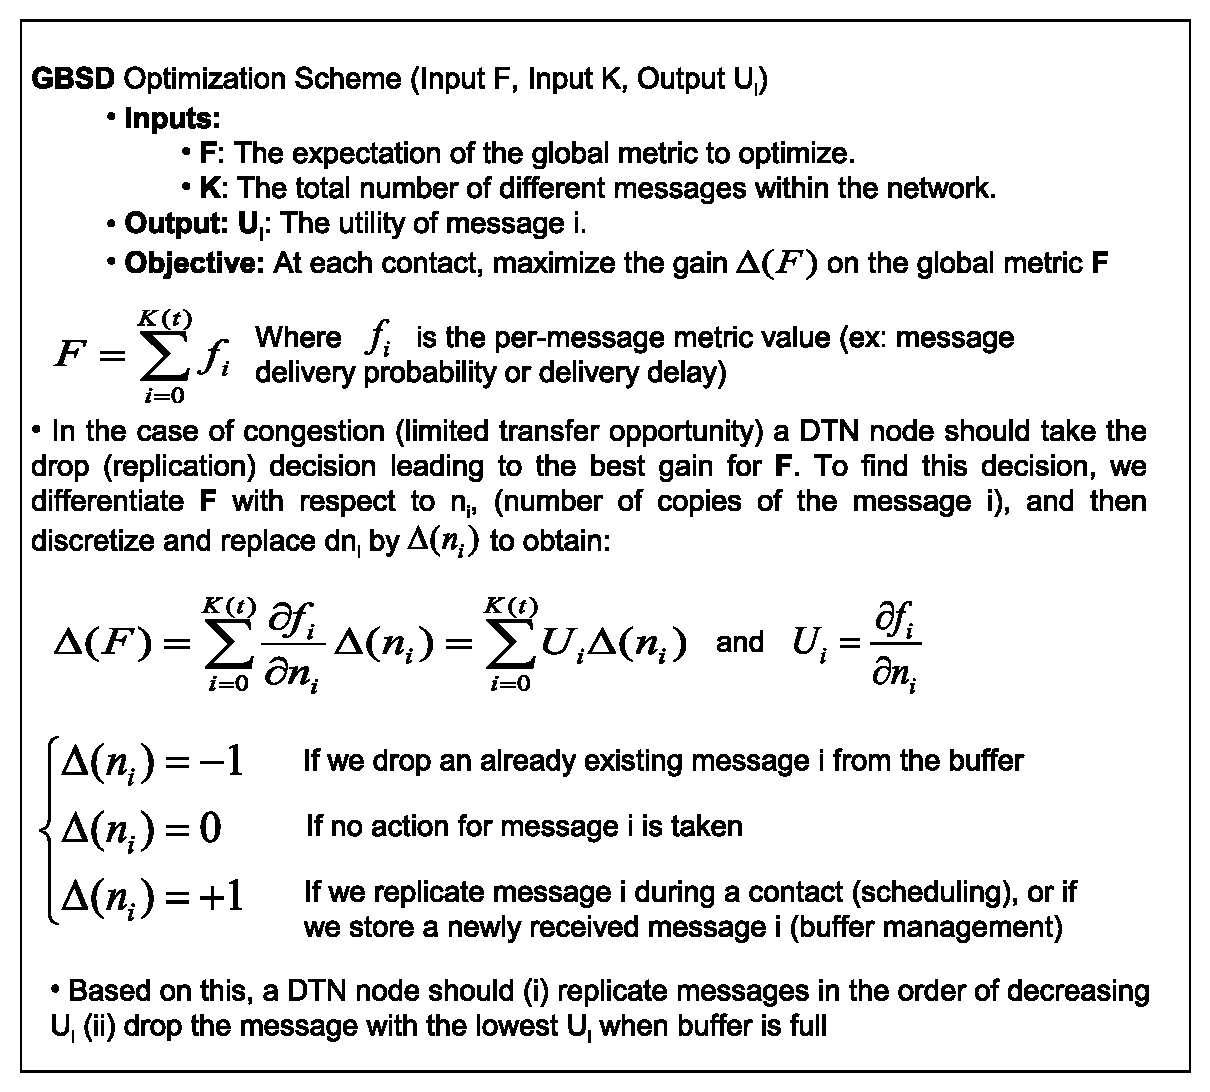
\includegraphics[width=3.1in,height=3in]{Chapitre3/GOS.eps}
\caption{GBSD Global optimization policy}
\label{GlobalOptimizationSchema}
\end{figure}

We will derive next such a per-message utility for two popular metrics: maximizing the average delivery probability (rate), and minimizing the average delivery delay. Table~\ref{table:notation} contains some useful notation that we will use throughout the paper. Finally, the GBSD optimization policy is summarized in Figure~\ref{GlobalOptimizationSchema}.

\begin{table}
\caption{Notation}
\centering
\label{table:notation}
\footnotesize
\begin{tabular}{|p{1.8cm}|p{5.7cm}|}
\hline
\bfseries Variable & \bfseries Description\\
\hline
L & Number of nodes in the network\\
\hline
K(t) & Number of distinct messages in the network at time $t$\\
\hline
$TTL_i$ & Initial Time To Live for message $i$\\
\hline
$R_i$ & Remaining Time To Live for message $i$\\
\hline
$T_i$ = $TTL_i$ - $R_i$ & Elapsed Time for message $i$. It measures the time since this message was generated by its source\\
\hline
$n_i(T_i)$ & Number of copies of message $i$ in the network after elapsed time $T_i$\\
\hline $m_i(T_i)$ & Number of nodes (excluding source) that
have \emph{seen} message $i$ since its creation until elapsed time $T_i$\\
\hline
$\lambda$ & Meeting \emph{rate} between two nodes; $\lambda = \frac{1}{E[H]}$ where $E[H]$ is the average meeting time\\
\hline
\end{tabular}
\end{table}
\normalsize

\subsection{Maximizing the average delivery rate}
\label{subsec:MaxAvgDeliveryRate}
We first look into a scenario where each message has a \emph{finite} $TTL$ value. The source of the message keeps a copy of it during the whole $TTL$ duration, while intermediate nodes are not obliged to do so. To maximize the average delivery probability among all messages in the network, the optimal policy must use the per message utility derived in the following theorem, in order to perform scheduling and buffer management.

\begin{theorem}\label{th:delivery-rate}
Let us assume that there are $K$ messages in the network, with
elapsed time $T_{i}$ for the message $i$. For each message $i \in [1,K]$, let $n_i(T_i)$ be the number of nodes who have a copy of the message at this time instant, and $m_i(T_i)$ those that have ``seen'' the message (excluding the source) since its creation\footnote{We say that a node \emph{A} has ''seen'' a message $i$, when $A$ had received a copy of message $i$ in the past, regardless of whether it still has the copy or has already removed it from its buffer.} ($n_i(T_i) \leqslant m_i(T_i)+1)$. To maximize the average delivery rate of all messages, a DTN node should apply the GBSD policy using the following utility per message $i$:
\begin{equation}\label{eq:GBSD-delivery-rate}
U_{i}(DR) = (1-\frac{m_i(T_i)}{L-1})\lambda R_i\exp(-\lambda n_i(T_i) R_i).
\end{equation}
\end{theorem}

The probability that a copy of a message $i$ will not be delivered by a node is given by the probability that the next meeting time with the destination is greater than $R_i$, the remaining lifetime of a message ($R_{i} = TTL - T_{i}$). This is equal to $\exp(-\lambda{R_i})$ under our assumptions.

Knowing that message $i$ has $n_i(T_i)$ copies in the network, and assuming that the message has not yet been delivered, we can derive the probability that the message itself will not be delivered (i.e. none of the $n_{i}$ copies gets delivered):
\begin{eqnarray}
P\{\mbox{message\ $i$ not\ delivered}\ |\ \mbox{not\ delivered\ yet}  \}= \nonumber \\
\prod_{k=1}^{n_i(T_i)}\exp(-\lambda R_i ) = \exp(-\lambda n_i(T_i) R_i).
\label{eq:p-not-delivered}
\end{eqnarray}

We need to also take into consideration what has happened in the network since the message generation, in the absence of an explicit delivery notification (this part is not considered in RAPID~\cite{Levine:Sigcomm07}, making the utility function derived there suboptimal). Given that all nodes including the destination have the same chance to see the message, the probability that a message $i$ has
been already delivered is equal to:

\begin{align}
P \{ \mbox{message\ $i$ already\ delivered} \} &=& m_i(T_i) / (L-1).
\label{eq:p-already-delivered}
\end{align}
Combining Eq.(\ref{eq:p-not-delivered}) and Eq.(\ref{eq:p-already-delivered}), the probability that a message $i$ will get delivered before its $TTL$ expires is:

\vspace{-0.4cm}
\small
\begin{align*}
P_i & =  P \{ \mbox{message\ $i$ not\ delivered\ yet} \} *  (1 -\exp(-\lambda n_i(T_i) R_i)) \\
& +  P \{ \mbox{message\ $i$ already delivered} \} \\
& =  (1 - \frac{m_i(T_i)}{L-1})*(1 - \exp(-\lambda n_i(T_i) R_i ))+\frac{m_i(T_i)}{L-1}.
\end{align*}
\normalsize

So, if we take at instant $t$ a snapshot of the network,
the global delivery rate for the whole network will be:

\vspace{-0.4cm}
\small
\begin{align*} DR =\sum_{i=1}^{K(t)}\left[(1 - \frac{m_i(T_i)}{L-1})*(1 -\exp(-\lambda n_i(T_i)  R_i )) +\frac{m_i(T_i)}{L-1}\right].
\end{align*}
\normalsize

In case of a full buffer or limited transfer opportunity, a
DTN node should take respectively a drop or replication decision that leads to the best gain in the global delivery rate DR. To define this optimal decision, we differentiate DR with respect to $n_i(T_i)$,

\small
\begin{align*}
\Delta(DR) &= \sum_{i=1}^{K(t)}{\frac{\partial P_i}{\partial n_i(T_i)} * \bigtriangleup n_i(T_i)}
\\&= \sum_{i=1}^{K(t)} \left[{(1-\frac{m_i(T_i)}{L-1})\lambda R_i\exp(-\lambda n_i(T_i) R_i) * \bigtriangleup n_i(T_i)}\right]
\end{align*}
\normalsize

Our aim is to maximize $\Delta(DR)$. In the case of message drop, for example, we know that: $\Delta n_i(T_i) = -1$ if we drop an already existing message $i$ from the buffer, $\Delta n_i(T_i) = 0$ if we don't drop an already existing message $i$ from the buffer, and $\Delta n_i(T_i) = +1$ if we keep and store the newly-received message $i$. Based on this, GBSD ranks messages using the per message utility in Eq.(\ref{eq:GBSD-delivery-rate}), then schedules and drops them accordingly. This utility can be viewed as the \emph{marginal utility value} for a copy of a message $i$ with respect to the total delivery rate. The value of this utility is a function of the global state of the message $i$ ($n_i$ and $m_i$) in the network.

As is evident from the above description, the GBSD policy is a greedy, locally optimal policy. However, greedy policies in general, are not guaranteed to converge to globally optimal outcomes. We will investigate the optimality properties of GBSD further in Section~\ref{OptimalityOfGradientPolicy}.

\subsection{Minimizing the average delivery delay}
\label{subsec:MinAvgDeliveryDelay}


We next turn our attention to minimizing the average delivery delay. We now assume that all messages generated have infinite $TTL$ or at least a $TTL$ value large enough to ensure a delivery probability close to $1$. The following
Theorem derives the optimal per-message utility, for
the same setting and assumptions as Theorem~\ref{th:delivery-rate}.

\begin{theorem} \label{th:delivery-delay}
To minimize the average delivery delay of all
messages, a DTN node should apply the GBSD policy using
the following utility for each message $i$:

\begin{equation}\label{eq:delivery-delay}
U_{i}(DD) = \frac{1}{n_i(T_i)^2 \lambda} ( 1-\frac{m_i(T_i)}{L-1}). \end{equation}
\end{theorem}

Let us denote the delivery delay for message $i$ with random variable $X_i$. This delay is set to $0$ (or any other constant value) if the message has been already delivered. Then, the total expected delivery delay ($DD$) for all messages for which copies still exist in the network is given by,

\small
\begin{align}\label{eq:DD1}
DD & = \sum_{i=1}^{K(t)} \left[\frac{m_i(T_i)}{L-1}*0 + (1 - \frac{m_i(T_i)}{L-1}) * E[X_i | X_i
> T_i]\right].
\end{align}
\normalsize

We know that the time until the first copy of the message $i$ reaches the destination follows an exponential distribution with mean $1/(n_i(T_i)
\lambda)$. It follows that,

\begin{align}\label{eq:DD2}
E[X_i | X_i
> T_i] &= T_i + \frac{1}{n_i(T_i) \lambda}.
\end{align}

Substituting Eq.(\ref{eq:DD2}) in Eq.(\ref{eq:DD1}), we get,

\begin{align*}
DD &= \sum_{i=1}^{K(t)} (1 - \frac{m_i(T_i)}{L-1})(T_i + \frac{1}{n_i(T_i)
\lambda}).
\end{align*}

Now, we differentiate $D$ with respect to $n_i(T_i)$ to find the policy that maximizes the improvement in $D$,

\begin{align*}
\Delta(DD) &= \sum_{i=1}^{K(t)}{\frac{1}{n_i(T_i)^2 \lambda} ( \frac{m_i(T_i)}{L-1}-1)* \Delta n_i(T_i)}.
\end{align*}

The best drop or forwarding decision will be the one that maximizes $\vert\Delta(DD)\vert$ (or $-\Delta(DD)$). This leads to the per message utility in Eq.(\ref{eq:delivery-delay}).


Note that, the per-message utility with respect to delivery delay is different than the one for the delivery rate. This implies (naturally) that both metrics cannot be optimized concurrently.

\subsection{The Case of Non-Homogeneous Mobility}
\label{section:heterogeneous-mobility}

Throughout our analysis, we have so far assumed homogeneous node mobility. Recent measurement studies have revealed that, often, different node pairs might have different meeting rates. We extend here our analytical framework, in order to derive per-message utilities that maximize the global performance metric, in face of such heterogeneous mobility scenarios. We illustrate the extension with the delivery rate\footnote{The treatment of delivery delay utilities does not involve Laplace transforms, but poses no extra difficulties. We thus omit it here, due to space limitations}. Specifically, we assume that meetings between a given node pair are exponentially distributed with meeting rate $\tilde{\lambda}$, where $\tilde{\lambda}$ is a \emph{random variable} such that:
\begin{equation*}
\tilde{\lambda} \in [0,\infty), \mbox{distributed as } f(\tilde{\lambda}).
\end{equation*}
$f(\tilde{\lambda})$ is a probability distribution that models the heterogeneous meeting rates between nodes, and can be any function integrable in $[0,\infty)$, capturing thus a very large range of conceivable mobility models.

The analysis of Theorem~\ref{th:delivery-delay} is thus modified as follows. Let's assume that message $i$ has $n_{i}$ copies in the network, and that the $n_{i}$ carriers have (unknown) meeting rates $\tilde{\lambda_{1}},\tilde{\lambda_{2}},\dots,\tilde{\lambda_{n_{i}}}$, respectively. Eq.(\ref{eq:p-not-delivered}) becomes:
\begin{eqnarray}
P\{\mbox{message\ $i$ not\ delivered}\ |\ \mbox{not\ delivered\ yet}  \}= \nonumber \\
E_{\tilde{\lambda_{1}},\tilde{\lambda_{2}},\dots,\tilde{\lambda_{n_{i}}}} [ \prod_{j=1}^{n_i}\exp(-\tilde{\lambda_{j}} R_i ) ] = \\
\prod_{j=1}^{n_i} \int_{0}^{\infty} \exp(-\tilde{\lambda_{j}} R_i ) f(\tilde{\lambda_{j}}) d\lambda_{j}  = (F_{\mathcal{L}}(R_{i}))^{n_{i}}, \label{eq:conditional-delivery}
\end{eqnarray}
where $F_{\mathcal{L}}(R_{i})$ is the Laplace transform of distribution $f(x)$ evaluated at $R_{i}$. Continuing as in the proof of Theorem~\ref{th:delivery-delay}, we get the unconditional probability of delivery $P_{i}$:
\begin{equation*}
P_{i} = (1 - \frac{m_i}{L-1})* (F_{\mathcal{L}}(R_{i}))^{n_{i}}+\frac{m_i}{L-1}.
\end{equation*}
Differentiating $P_{i}$ with respect to $n_{i}$, we derive the following generic marginal utility per message:
\begin{equation} \label{eq:general-utility-delivery}
(1 - \frac{m_i}{L-1}) * \ln(F_{\mathcal{L}}(R_{i})) * (F_{\mathcal{L}}(R_{i}))^{n_{i}}.
\end{equation}

We now consider some example distributions for node meeting rates, and derive the respective marginal utility.

\emph{Dirac delta funtion}: Let $f(\tilde{\lambda}) = \delta(\tilde{\lambda} - \lambda)$, where $\delta(x)$ is an impulse function (Dirac's delta function). This corresponds to the case of homogeneous mobility, considered earlier, with average meeting rates for all nodes equal to $\lambda$. The laplace distribution of $f(\tilde{\lambda})$ is then equal to $F_{\mathcal{L}}(R_{i}) = \exp(-\lambda R_{i})$. Replacing this in Eq.(\ref{eq:general-utility-delivery}), the generic marginal utility, gives us Eq.(\ref{eq:GBSD-delivery-rate}), the utility for homogeneous mobility, as expected.

\emph{Exponential distribution}: Let $f(\tilde{\lambda}) = \lambda_{0} \exp(-\tilde{\lambda} \lambda_{0})$, for $\tilde{\lambda} \ge 0$. This corresponds to a mobility model, where individual rates between pairs differ, but the variance of these rates is not high and their average is equal to $\lambda_0$. The laplace transform of $f(\tilde{\lambda})$ is
\begin{equation*}
F_{\mathcal{L}}(R_{i}) = \frac{1}{(R_{i} + \lambda_{0})^{2}}.
\end{equation*}
Replacing this in Eq.(\ref{eq:general-utility-delivery}) gives us the marginal utility per message that should be used:
\begin{equation}
(1 - \frac{m_i}{L-1}) * \ln(\frac{1}{(R_{i} + \lambda_{0})^{2}}) * \frac{1}{(R_{i} + \lambda_{0})^{2n_{i}}}.
\end{equation}

\emph{Unknown distribution in large networks}: If the actual probability distribution of meeting rates is not known, the following approximation could be made in order to derive marginal utilities per message and use them for buffer management. Let us assume that the meeting rates come from an unknown distribution with first and second moments $\bar{\lambda}$ and $\sigma^{2}$, respectively. Let us further assume that there is a large number of nodes, such that $n_{i}$, the number of copies of message $i$ at steady state, is large. Using the central limit theorem, we have:
\begin{equation}
Prob(\sum_{j=1}^{n_{i}} \tilde{\lambda_{j}} \le \lambda) \underset{n_{i} \rightarrow \infty}{\sim} \mathcal{N}(n_{i}\bar{\lambda}, \sigma \sqrt{n_{i}}),
\end{equation}
that is, the sum of meeting rates with the destination of the $n_{i}$ relays for message $i$ is (approximately) normally distributed. Replacing this in Eq.(\ref{eq:conditional-delivery}), we get the (unconditional) delivery probability $P_{i}$
\begin{eqnarray*}
P_{i} = (1 - \frac{m_i}{L-1})* F_{\mathcal{L}}(R_{i}) + \frac{m_i}{L-1},
\end{eqnarray*}
where $F_{\mathcal{L}}(R_{i})$ is the Laplace transform of the above normal distribution\footnote{Note that the Laplace transform is not raised anymore to the $n_{i}^{\mbox{th}}$ power, as the distribution already corresponds to the sum of all rates.}. After some algebraic manipulations we can get the new marginal utility for message $i$:
\footnotesize
\begin{equation}
(1 - \frac{m_i}{L-1}) * \frac{ (\bar{\lambda}^{2} \sqrt{8} (n_{i})^{-\frac{1}{2}} + \sqrt{2} \sigma^{2} (n_{i})^{-\frac{5}{2}}) \exp( n_{i} \frac{\bar{\lambda}^{2}}{\sigma^{2}} + \frac{R_{i}^{2}}{4} )}{8 \sigma^{4}} * \mbox{erfc}(\frac{R_{i}}{2}).
\end{equation}
\normalsize

In a large enough network, even if the actual distribution of meeting rates is not known, a node could still derive good utility approximations, by measuring and maintaining an estimate for the first and second moments of observed or reported meeting rates (e.g. with techniques similar to the ones discussed in the next Section). Furthermore, the homogeneous assumption could be considered as a useful approximation for large networks where the common rate is taken as $\bar{\lambda}$. Additional complexity in the mobility model (e.g. correlated meeting rates) could still be handled in our framework, yet at the expense of ease of interpretation (and thus usefulness) of the respective utilities. We will therefore consider the simple case of homogeneous mobility for the remainder of our discussion, in order to better elucidate some additional key issues related to buffer management in DTNs, and resort to a simulation-based validation under realistic mobility patterns.

\subsection{Optimality of Gradient Ascent Policy}
\label{OptimalityOfGradientPolicy}
We finally turn our attention back to the distributed (\emph{local}) buffer management policies of Sections~\ref{subsec:MaxAvgDeliveryRate} and~\ref{subsec:MinAvgDeliveryDelay}, in order to further investigate their optimality. Let us observe our network at a random time instant, and assume there are $K$ total undelivered messages, with remaining Times To Live $R_{1}, R_{2}, \dots, R_{K}$, respectively. The centralized version of our buffer management problem then consists of assigning the available buffer space across the network ($L$ nodes each able to store $B$ message copies) among the copies of these messages, $n_{1}, n_{2}, \dots, n_{K}$, so as to maximize the expected delivery probability for all these messages (where the expectation is taken over mobility decisions of all nodes). This corresponds to the following optimization problem:
\begin{eqnarray}
\underset{n_{1},n_{2},\dots,n_{K}}{\max} \sum_{i=1}^{K} (1-\exp(-\lambda n_i R_i)) \label{eq:optimization-function} \\
\sum_{i=1}^{K} n_{i} - L B \le 0 \label{eq:capacity-constraint} \\
n_{i} - L  \le 0, \forall i \label{eq:max-copy-constraint} \\
n_{i} \geq 1, \forall i \label{eq:min-copy-constraint}
\end{eqnarray}

This is a constrained optimization problem, with $K$ variables and $2K+1$ inequality constraints. The optimization function in Eq.(\ref{eq:optimization-function}) is a concave function in $n_{i}$. Constraint in Eq.(\ref{eq:capacity-constraint}) says that the total number of copies (for all messages) should not exceed the available buffer space in all $L$ nodes, and is linear. Finally, the $2K$ constraints of Eq.(\ref{eq:max-copy-constraint}) are also linear, and simply say that there is no point for any node to store two copies of the same message. Consequently, if we assume that $n_{i}$ are real random variables (rather than integers), this is a \emph{convex optimization} problem, which can be solved efficiently~\cite{Boyd:convex-optimization-book} (but not easily analytically).

%Introducing Lagrange multipliers, the problem in hand then becomes that of (in regulal form)
%\footnotesize
%\begin{eqnarray}
%\min \sum_{i=1}^{K} (\exp(-\lambda n_i R_i) -1) + \beta (\sum_{i=1}^{K} n_{i} - L B) + \sum_{i=1}^{K} \gamma_{i} (n_{i} - L),
%\end{eqnarray}
%\normalsize
%where $\beta$, and $\gamma_{i}$ are non-negative Lagrange multipliers for each inequality in the original form.

Having found an optimal vector $\mathbf{n}$, a centralized optimal algorithm can easily assign the copies to different nodes (e.g. picking nodes sequentially and filling their buffers up with any non-duplicate copy, starting from the messages with highest assigned $n_{i}$ --- due to uniform mobility the choice of specific nodes does not matter). It is important to note that, given this assignment, \emph{no further message replication or drop is needed. This is the optimal resource allocation averaged over all possible future node movements.} The optimal algorithm must perform the same process at every subsequent time step in order to account for new messages, messages delivered, and the smaller remaining times of undelivered messages.

Our local policies offer a \emph{distributed implementation of a gradient ascent algorithm for this problem}. Gradient ascent algorithms look at the current state, i.e. vector $\mathbf{n}(k)$ at step $k$, and choose a neighboring vector $\mathbf{n}(k+1)$ that improves the optimization function in Eq.(\ref{eq:optimization-function}), and provably converge to the optimal solution~\cite{Boyd:convex-optimization-book}. In our case, a step corresponds to a \emph{contact} between two nodes, and the neighboring states and permitted transitions depend on the messages in the buffers of the two nodes in contact. In other words, our gradient ascent algorithm is supposed to make enough steps to converge to the optimal copy vector $\mathbf{n^{*}}$, before the state of the network (i.e. number and ID of messages) changes enough for the optimal assignment to change significantly. This depends on the rate of update steps ($\approx \lambda L^{2}$) and the message TTL. If $TTL * \lambda * L^{2} \gg 1$, then we expect the distributed, local policy to be able to closely follow the optimal solution at any time $t$. In Section~\ref{GBSD:Optimality}, we use simulation to prove that this is indeed the case for the scenarios considered.

\section{Using Network History to Approximate Global Knowledge in Practice}
\label{sec:learning}

It is clear from the above description that the optimal policy (GBSD) requires global information about the network and the ''spread'' of messages, in order to optimize a specific routing metric. In particular, for each message present in a node's buffer, we need to know the values of $m_i(T_i)$ and $n_i(T_i)$. In related work~\cite{Levine:Sigcomm07}, it has been suggested that this global view could be obtained through a secondary, ``instantaneous'' channel (e.g. cellular network), if available, or by flooding (``in-band'') all necessary meta-data. Regarding the former option, cellular network connections are known to be low bandwidth (measurements suggest only few kbps even for 2.5-3G technologies~\cite{Keshav:multi-nic}) and high cost in terms of power and actual monetary cost per bit. In networks of more than a few nodes, the amount of signalling data might make this option prohibitive. Concerning flooding, our experiments show that the impact of the flooding delay on the performance of the algorithm is not negligible. In practice, intermittent network connectivity and the long time it takes to flood buffer status information across DTN nodes, make this approach inefficient.

A different, more robust approach is to find estimators for the unknown quantities involved in the calculation of message utilities, namely $m$ and $n$. We do this by designing and implementing a learning process that permits a DTN node to gather knowledge about the global network state at different times in the past, by making in-band exchanges with other nodes. Each node maintains a list of encountered nodes and the state of each message carried by them as a function of time (i.e. its buffer state history). Specifically, it logs whether a given message was present at a given time $T$ in a node's buffer (counting towards $n$) or whether it was encountered earlier but is not anymore stored, e.g. it was dropped (counting towards $m$). In Section~\ref{sec:NetworkHistory}, we describe our statistics maintenance and collection method, in more detail, along with various optimizations to considerably reduce the signalling overhead.

Since global information gathered thus about a specific message might take a long time to propagate (as mentioned earlier) and hence might be obsolete when we calculate the utility of the message, we follow a different route. Rather than looking for the current value of $m_{i}(T)$ and $n_{i}(T)$ \emph{for a specific message $i$} at an elapsed time $T$, we look at what happens, \emph{on average, for all messages after an elapsed time $T$}. In other words, the $m_i(T)$ and $n_i(T)$ values for message $i$ at elapsed time $T$ are estimated using measurements of $m$ and $n$ for the same elapsed time $T$ but \emph{measured for (and averaged over) all other older messages}. These estimations are then used in the evaluation of the per-message utility.

%Next, we present the later estimators and in Section~\ref{NetworkHistory} we describe the practical model we propose to maintain the statistics related to the network history as well as the statistics collection method that we propose to use in order to keep up-to-date these statistics.

Let's denote by $\stackrel{\wedge}{n}(T)$ and
$\stackrel{\wedge}{m}(T)$ the estimators for $n_i(T)$ and $m_i(T)$ of message $i$. For the purpose of the analysis, we suppose that the variables $m_{i}(T)$ and $n_{i}(T)$ at elapsed time $T$ are instances of the random variables $N(T)$ and $M(T)$. We develop our estimators $\stackrel{\wedge}{n}(T)$ and $\stackrel{\wedge}{m}(T)$ so that when plugged into the GBSD's delivery rate and delay per-message utilities calculated in Section~\ref{sec:optimal-policy}, we get two new per-message utilities that can be used by a DTN node without any need for global information about messages. This results in a new scheduling and drop policy, called HBSD (History Based
Scheduling and Drop), a deployable variant of GBSD that uses the same algorithm, yet with per-message utility values calculated using estimates of $m$ and $n$.

\subsection{Estimators for the Delivery Rate Utility}
\label{sec:learning:EDR}

When global information is unavailable, one can calculate the
average delivery rate of a message over all possible values of
$M(T)$ and $N(T)$, and then try to maximize it. In the framework of the GBSD policy, this is equivalent to choosing the estimators $\stackrel{\wedge}{n}(T)$ and
$\stackrel{\wedge}{m}(T)$ so that the calculation of the average delivery rate is unbiased:

\begin{align*}
E[(1 - \frac{M(T)}{L-1})*(1 -\exp(-\lambda N(T) R_i
))+\frac{M(T)}{L-1}]&=
\\(1 -
\frac{\stackrel{\wedge}{m}(T)}{L-1})*(1 -\exp(-\lambda
\stackrel{\wedge}{n}(T) R_i
))+\frac{\stackrel{\wedge}{m}(T)}{L-1}
\end{align*}

Plugging any values
for $\stackrel{\wedge}{n}(T)$ and $\stackrel{\wedge}{m}(T)$ that verify this equality into the expression for the per-message utility of Eq.(~\ref{eq:GBSD-delivery-rate}), one can make sure that the obtained policy maximizes the average delivery rate. This is exactly our purpose. Suppose now that the best estimator for $\stackrel{\wedge}{m}(T)$ is its average, i.e., $\stackrel{\wedge}{m}(T)=\stackrel{-}{m}(T)=E[M(T)]$. This approximation is driven by the observation we made that the
histogram of the random variable $M(T)$ can be  approximated by a Gaussian distribution with good accuracy. To confirm this, we have applied the Lillie test~\cite{LillieTest}, a robust version of the well known Kolmogorov-Smirnov goodness-of-fit test, to $M(T)$ for different elapsed times ($T$ = 25\%,50\% and 75\% of the $TTL$). This test led to acceptance for a 5\% significance level. Consequently, the average of $M(T)$ is at the same time the unbiased estimator and the most frequent value among the vector $M(T)$. Then, solving for $\stackrel{\wedge}{n}(T)$ gives:

\begin{align}
\stackrel{\wedge}{n}(T) = -\frac{1}{\lambda R_i}
\ln(\frac{E[(1-\frac{M(T)}{L-1})\exp(-\lambda N(T)
R_i)]}{(1-\frac{\stackrel{-}{m}(T)}{L-1})})
\end{align}

Substituting this expression into Eq.(\ref{eq:GBSD-delivery-rate}) we obtain the following new per message utility for our approximating HBSD policy:

\begin{align}
\label{HBSD-DR-U}
\lambda R_i E[(1-\frac{M(T)}{L-1})\exp( - \lambda R_i N(T))]
\end{align}

The expectation in this expression is calculated by summing over all known values of $N(T)$ and $M(T)$ for past messages at elapsed time $T$. Unlike Eq.(\ref{eq:GBSD-delivery-rate}), this new per-message utility is a function of past history of messages and can be calculated locally. It maximizes the average message delivery rate calculated over a large number of messages. When the number of messages is large enough for the law of large numbers to work, our history based policy should give the same result as that of using the real global network information.

Finally, we note that $L$, the number of nodes in the network, could also be calculated from the statistics maintained by each node in the network. In this work, we assume it to be fixed and known, but one could estimate it similar to $n$ and $m$, or using different estimation algorithms like the ones proposed in~\cite{PellegriniAOC2009}.

\subsection{Estimators for the Delivery Delay Utility}
\label{sec:learning:EDD}
Similar to the case of delivery rate, we calculate the estimators $\stackrel{\wedge}{n}(T)$ and
$\stackrel{\wedge}{m}(T)$ in such a way that the average delay is not affected by the estimation. This gives the following per-message utility specific to HBSD,

\begin{align}
\label{HBSD-DD-U}
\frac{E[\frac{L-1-M(T)}{N(T)}]^2}{\lambda
(L-1)(L-1-\stackrel{-}{m}(T))}
\end{align}

This new per-message utility is only a function of the locally available history of old messages and is thus
independent of the actual global network state. For large number of messages, it should lead to the same average delay
as when the exact values for $m$ and $n$ are used.


\section{Performance Evaluation}
\label{sec:sims}

\subsection{Experimental Setup}
\label{sec:ExperimentalSetup}

To evaluate our policies, we have implemented a DTN framework into the Network Simulator NS-2~\cite{DTN-NS2}. This implementation includes (i) the Epidemic routing protocol with \emph{FIFO} for scheduling messages queued during a contact and \emph{drop-tail} for message drop, (ii) the RAPID routing protocol based on
flooding (i.e. no side-channel) as described, to our best
understanding, in~\cite{Levine:Sigcomm07}, (iii) a new version of Epidemic routing enhanced with our optimal joint scheduling and drop policy (GBSD), (iv) another version using our statistical learning based distributed algorithm (HBSD), and (v) the VACCINE anti-packet mechanism described
in~\cite{Towsley:Epidemic}\footnote{We have also performed simulations without any anti-packet mechanism, from which similar conclusions can be drawn.}.

In our simulations, each node uses the 802.11b protocol to communicate, with rate 11Mbits/sec. The transmission range is 100 meters, to obtain network scenarios that are neither fully connected (e.g. MANET) nor extremely sparse. 

Our simulations are based on five mobility scenarios: two synthetic mobility models and three real-world mobility traces.

\emph{Synthetic Mobility Models:} We've considered both the Random Waypoint mobility model and the HCMM model~\cite{HCMM}. The later is inspired from Watts' Caveman model that was shown to reproduce statistics of human mobility, such as inter-contact times and contact duration.

\emph{Real Mobility Traces:} The first \emph{(i)} real trace is the one collected as part of the ZebraNet wildlife tracking experiment in Kenya and described in~\cite{ZebraNetMovement}. The second mobility trace tracks San Francisco's Yellow Cab taxis. Many cab companies outfit their cabs with \emph{GPS} to aid in rapidly dispatching
cabs to their costumers. The Cabspotting system~\cite{Cabspotting} talks to the Yellow Cab server and stores the data in a database. We have used an API provided by the Cabspotting system in order to extract mobility traces\footnote{Note that this trace describes taxi's positions according to the \emph{GPS} cylindrical coordinates (\emph{Longitude}, \emph{Latitude}. In order to uses these traces as input for the NS-2 simulator, we have implemented a tool~\cite{DTN-NS2} based on the Mercator cylindrical map projection which permit us to convert traces to plane coordinates.}. And finally, the third \emph{(iii)} trace consists on the KAIST real mobility trace collected from a university campus (KAIST) in South Korea~\cite{KAIST}. We consider a sample of the KAIST campus trace taken from 50 students, where the GPS receivers log their position at every 30 seconds. 

To each source node, we have associated a CBR (Constant Bit Rate) application, which chooses randomly from [0, $TTL$] the time to start generating messages of $5KB$ for a randomly chosen destination. We have also considered other message sizes (see e.g.~\cite{KrifaBS08}), but found no significant differences in the qualitative and quantitative conclusions drawn regarding the relative performance of different schemes\footnote{In future work, we intend to evaluate the effect of variable message size and its implications for our optimization framework. In general, utility-based scheduling problems with variable sized messages can often be mapped to Knapsack problems (see e.g.~\cite{Boldrini:MSWIM08}).}.
Unless otherwise stated, each node maintains a buffer with a capacity of $20$ messages to be able to push the network towards a congested state without exceeding the processing and memory capabilities of our simulation cluster. We compare the performance of the various routing protocols using the following two metrics: the average delivery rate and average delivery delay of messages in the case of infinite $TTL$\footnote{By infinite TTL, we mean any value large enough to ensure almost all messages get delivered to their destination before the TTL expires.}. Finally, the results presented here are averages from 20 simulation runs, which we found enough to ensure convergence.

\subsection{Performance evaluation for delivery rate}
\label{sec:sims:DR}

First, we compare the delivery rate of all
policies for the three scenarios shown in Table~\ref{SP}.

\begin{table}[!h]
\renewcommand{\arraystretch}{1.1}
\caption{Simulation parameters}
\centering
\begin{tabular}{|p{4cm}|p{1.5cm}|p{1.5cm}|p{1.5cm}|p{1.5cm}|p{1.5cm}|}
\hline
\bfseries Mobility pattern: & RWP & ZebraNet & Taxis & KAIST& HCMM \\
\hline
Sim. Duration(h):& 7 & 14 & 42 & 24 & 24\\
\hline
Sim. Area ($km^2$):& 3*3 & 3*3 & - & - & 5*5\\
\hline
Nbr. of Nodes: & 70 & 70 & 70 & 50 & 70\\
\hline
Avg. Speed (m/s):& 2 & - & - & - & -\\
\hline
$TTL(h)$:& 1 & 2 & 6 & 4 & 4\\
\hline
CBR Interval(s):& 360 & 720 & 2160 & 1440& 1440\\
\hline
\end{tabular}
\label{SP}
\end{table}

\begin{figure}[!h]
\centering
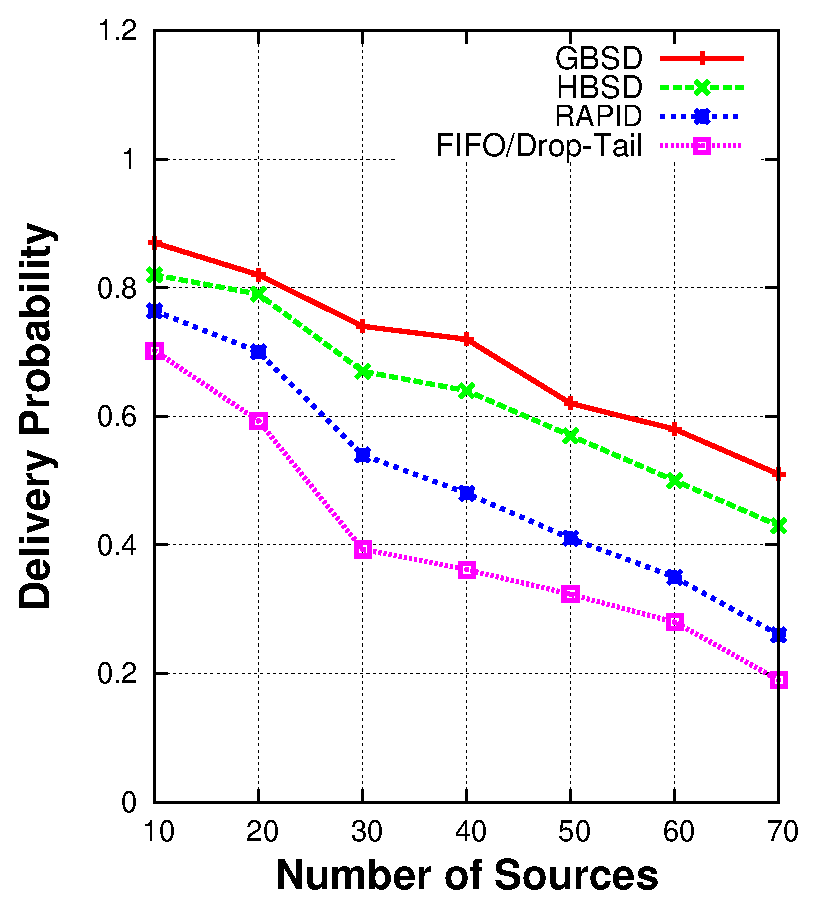
\includegraphics[width=3in,height=2.2in]{Chapitre3/fig2.eps}
\small
\caption{Delivery Probability for Epidemic Routing with different scheduling and drop policies (both buffer and bandwidth constraints).}\normalsize
\label{DR-RWP}
\end{figure}

\begin{figure}[!h]
\centering
\includegraphics[width=3in,height=2.2in]{Chapitre3/fig22.eps}
\small
\caption{Delivery Probability (KAIST mobility trace).}
\normalsize
\label{DR-KAIST}
\end{figure}

\begin{table}[!h]
\renewcommand{\arraystretch}{1.1}
\caption{Taxi Trace \& Limited buffer and bandwidth}
\centering
\footnotesize
\begin{tabular}{|p{2.5cm}||p{0.9cm}||p{0.9cm}||p{0.9cm}||p{1.5cm}|}
\hline
\bfseries Policy: & GBSD & HBSD & RAPID & FIFO\textbackslash DT\\
\hline\hline
D. Probability:&0.72 &0.66 &0.44 &0.34\\
\hline\hline
D. Delay(s):&14244&15683&20915&36412\\
\hline
\end{tabular}
\label{T-LB+LB}
\end{table}

\begin{table}[!h]
\renewcommand{\arraystretch}{1.1}
\caption{ZebraNet Trace \& Limited buffer and bandwidth}
\centering
\footnotesize
\begin{tabular}{|p{2.5cm}||p{0.9cm}||p{0.9cm}||p{0.9cm}||p{1.5cm}|}
\hline
\bfseries Policy: & GBSD & HBSD & RAPID & FIFO\textbackslash DT\\
\hline\hline
D. Probability:&0.68&0.59&0.41&0.29\\
\hline\hline
D. Delay(s):&4306&4612&6705&8819\\
\hline
\end{tabular}
\label{ZebraNetResults}
\end{table}


\begin{table}[!h]
\renewcommand{\arraystretch}{1.1}
\caption{HCMM Trace (70 CBR sources)}
\centering
\footnotesize
\begin{tabular}{|p{1.8cm}|p{0.9cm}|p{0.9cm}|p{0.9cm}|p{1.5cm}|}
\hline
\bfseries Policy: & GBSD & HBSD & RAPID & FIFO\textbackslash DT\\
\hline
D. Probability:&0.62&0.55&0.38&0.23\\
\hline
D. Delay(s):&3920&4500&6650&8350\\
\hline
\end{tabular}
\label{HCMM-Results}
\end{table}

Figure~\ref{DR-RWP} shows the delivery rate based on the Random Waypoint model. From this plot, it can be seen that: the GBSD policy plugged into
Epidemic routing gives the best performance for all numbers of
sources. When congestion-level decreases, so does the difference
between GBSD and other protocols, as expected. Moreover, the HBSD
policy also outperforms existing protocols (RAPID and Epidemic based on FIFO/drop-tail) and performs very close to the optimal GBSD. Specifically, for $70$ sources, HBSD offers an almost 60\% improvement in delivery rate compared to RAPID and is only 14\% worse than GBSD. Similar conclusions can be also drawn for the case of the real Taxi trace,  ZebraNet trace, KAIST trace or the HCMM model and $70$ sources. Results for these cases are respectively summarized in Table~\ref{T-LB+LB}, Table~\ref{ZebraNetResults}, Figure~\ref{DR-KAIST} and Table~\ref{HCMM-Results}.

\subsection{Performance evaluation for delivery delay}
\label{sec:sims:DD}

To study delays, we increase messages' TTL (and simulation duration), to ensure almost every message gets delivered, as follows. Random Waypoint: (duration 10.5h, TTL = 1.5h). ZebraNet: (simulation duration = 28h, TTL = 4h). Taxi trace:  (simulation duration = 84h, TTL = 12h). Traffic rates are as in Section~\ref{sec:sims:DR}.

\begin{figure}[!h]
\centering
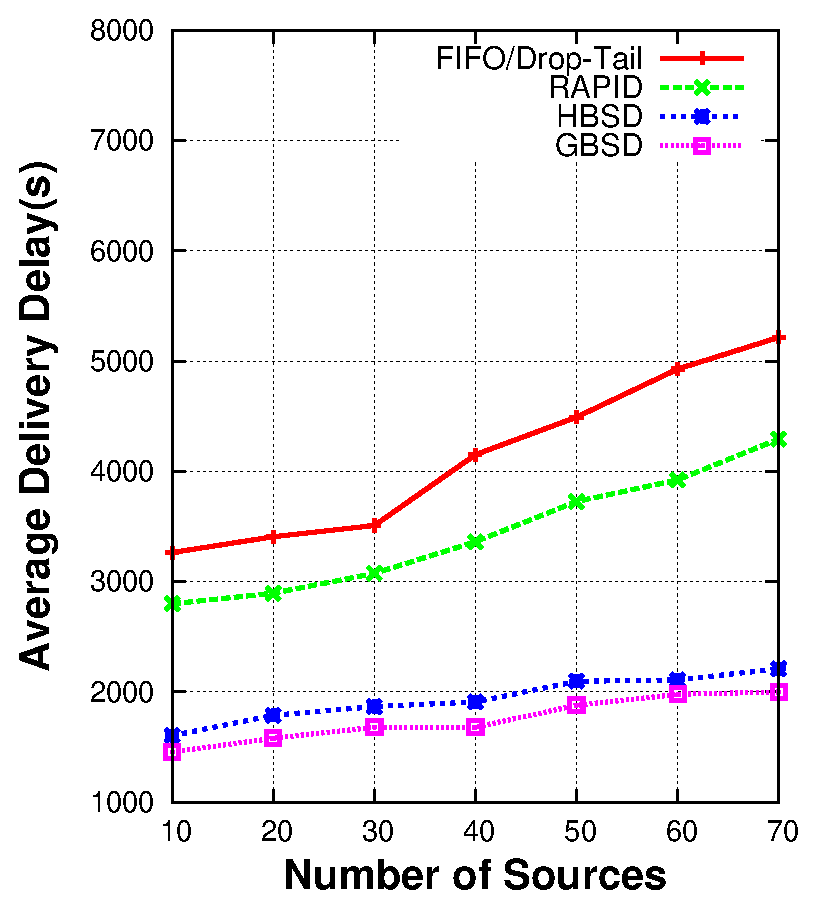
\includegraphics[width=3in,height=2.2in]{Chapitre3/fig3.eps}
\caption{Delivery Delay for Epidemic Routing with different scheduling and drop policies (both buffer and bandwidth constraints).}
\label{DD-RWP}
\end{figure}

\begin{figure}[!h]
\centering
\includegraphics[width=3in,height=2.2in]{Chapitre3/fig33.eps}
\caption{Delivery Delay (KAIST mobility trace).}
\label{DD-KAIST}
\end{figure}

For the random waypoint mobility scenario, Figure~\ref{DD-RWP} depicts the
average delivery delay for the case of both limited buffer and
bandwidth. As in the case of delivery rate, GBSD gives the best
performance for all considered scenarios. Moreover, the HBSD policy
outperforms the two routing protocols (Epidemic based on
FIFO/drop-tail, and RAPID) and performs close to GBSD. Specifically,
for 70 sources and both limited buffer and bandwidth, HBSD average
delivery delay is 48\% better than RAPID and only 9\% worse than
GBSD.

Table~\ref{T-LB+LB}, Table~\ref{ZebraNetResults}, Figure~\ref{DD-KAIST} and Table~\ref{HCMM-Results} show that similar conclusions can be drawn for the delay under respectively the real Taxi(s), ZebraNet trace, KAIST trace and the HCMM model. 

\subsection{Optimality}
\label{GBSD:Optimality}

\begin{figure}[!h]
\centering
\includegraphics[width=3in,height=2.2in]{Chapitre3/AvgDistancePerCoordinate.eps}
\caption{Normalized Manhattan distance between two consecutive N optimal vectors.}
\label{Sensitivity}
\end{figure}

\begin{figure}[!h]
\centering
\includegraphics[width=3in,height=2.2in]{Chapitre3/NbrCopiesDiff.eps}
\caption{Difference in terms of Nbr of copies.}
\label{DiffinTermsOfNbrCopies}
\end{figure}

Here, we use simulations results (based on the RW scenario) that our proposed policy (GBSD) can ``keep up'' with the optimal algorithm described in Section~\ref{OptimalityOfGradientPolicy}. Figure~\ref{Sensitivity} plots the normalized Manhattan distance $d(X,Y) = \frac{\sum_{i=1}^{K}|x_i - y_j|}{K}$ between two consecutive optimal copy vectors, resulting from solving the optimal centralized version offline. These optimal vectors are calculated every $4ms$, corresponding to the average time between any two consecutive contacts among the network. As is evident in the figure, this distance is very small, implying that our distributed gradient-ascent implementation of this policy (GBSD/HBSD) has enough time to converge to the optimal vector, before this changes significantly. In order to further validate the optimality of our policy, we compare in Figure~\ref{DiffinTermsOfNbrCopies} the absolute difference between the number of copies assigned to a message by our GBSD policy and the number of copies allocated to the same message by the optimal algorithm~\ref{OptimalityOfGradientPolicy}. We have picked some messages randomly and plot this difference along a time window in their lifetime. These results show that the GBSD policy stays is able to follow the optimal one with an average error of $1-2$ copies allocated at most. We believe this result consolidates the optimality properties of our proposed distributed implementation of the optimal policy.

\section{Maintaining Network History}
\label{sec:NetworkHistory}

The results of the previous section clearly show that our distributed policy (HBSD) that uses estimators of global message state (rather than actual state) successfully approximates the performance of the optimal policy (GBSD). This is as an important step towards a practical implementation of efficient buffer management and scheduling algorithms on wireless devices. Nevertheless, in order to derive good estimators in a distributed manner, nodes need to exchange (a possibly large amount of) metadata during every node meeting. Potentially, each node needs to know the history of all messages having passed through a node's buffer, for every node in the network. In a small network, the amount of such ``control'' data might not be much, considering that large amounts of data transfers can be achieved between 802.11 transceivers during short contacts (data transfers of a few $10s$ of MBytes have been reported for experiments between vehicles moving at high speeds~\cite{Keshav:Mobisys07}). Nevertheless, in larger networks, this method can quickly become unsalable and interfere with (or starve) data transmissions, if statistics maintenance and collection is naively done.

In this section, we describe the type of statistics each node maintains towards calculating the HBSD utility for each message, and propose a number of mechanisms and optimizations to significantly reduce (and control) the amount of metadata exchanged during contacts. Finally, we explore the impact of reducing the amount of collected statistics on the performance of our buffer management and scheduling policy. Our results suggest that, with a carefully designed statistics collection and maintenance scheme, order(s) of magnitude less metadata can be exchanged (compared to maintaining a complete view about the network), without significantly affecting performance.

\subsection{Maintaining Buffer State History}
\label{NetworkHistoryModel}

In order to keep track of the statistics about past messages necessary to assign appropriate utility values to messages considered for transmission or dropping, we propose that each node maintains the data structure depicted in Figure~\ref{NHM}. Each node maintains a list of messages whose history in the network it keeps track of (we will see in the next section how a node chooses which messages to include in this list). For each message, it maintains its $ID$ (a unique string resulting from the combination of some of its attributes), its $TTL$ and the list of nodes that have \emph{seen} it before (i.e. had stored the messages at some time in the past and should be accounted towards calculating $m$ or $n$). Then, for each of the nodes in the list, it maintains a data structure with the following data: (i) the node's $ID$, (ii) a boolean array $Copies\_Bin\_Array$, and (iii) the version $Stat\_Version$ associated to this array.

The $Copies\_Bin\_Array$ array (Figure~\ref{BA}) enables nodes to maintain dynamically what each message experienced during its life time. For a given entry pair (message $a$ and node $b$) in this list, the $Copies\_Bin\_Array[k]$ indicates if the node $a$ had already stored or not a copy of message $b$ in its buffer during \emph{Bin} $k$. In other words, time is quantized into ``bins'' of size $Bin\_Size$, and bin $k$ correspond to the period of time between $k*Bin\_Size$ and $(k+1)*Bin\_Size$. As a result, the size of the $Copies\_Bin\_Array$ is equal to $TTL/Bin\_Size$.

How should one choose $Bin\_Size$? Clearly, the larger it is, the fewer the amount of data a node needs to maintain and to exchange during each meeting; however, the smaller is also the granularity of values the utility function can take and thus the higher the probability of an incorrect (scheduling or buffer management) decision. As already described in Section~\ref{sec:optimal-policy}, message transmissions can occur only when nodes encounter each other. This is also the time granularity at which buffer state changes occur. Hence, we believe that a good trade-off is to monitor the evolution of each message's state at a bin granularity in the order of meeting times\footnote{According to the \emph{Nyquist-Shannon}~\cite{Nyquist} sampling theorem, a good approximation of the size of a \emph{Bin} would be equal to inter-meeting-time/2. A running average of the observed times between consecutive meetings could be maintained easily, in order to dynamically adjust the bin size~\cite{akis:ton-multi}.}. This \emph{already results in a big reduction of the size of statistics to maintain locally} (as opposed to tracking messages at seconds or milliseconds granularity), while still enabling us to infer the correct messages statistics.

Finally, the $Stat\_Version$ indicates the Bin at which the last update occurred. Let's assume that a message $a$ is first stored at a node $b$ during bin $3$. It then creates a new entry in its list for pair ($a$,$b$), inserts $0$s in bins $0-2$ of the new $Copies\_Bin\_Array$ and $1$s in the rest of the bins, and sets the $Stat\_Version$ to $3$. If later, at in bin $5$ node $b$ decides to drop this message, then the list entry is maintained, but it sets all bins from $5$ to $TTL/Bin\_Size$ to $0$, and updates the $Stat\_Version$ to $5$. Finally, when the TTL for message $a$ elapses (regardless of whether $a$ is still present in $b$'s buffer or not), $b$ sets the $Stat\_Version$ to $TTL/Bin\_Size$, which also indicates that all information about the history of \emph{this} message in \emph{this} buffer is now available. The combination of how the $Copies\_Bin\_Array$ is maintained and the $Stat\_Version$ updated, ensures that only the minimum amount of necessary metadata \emph{for this pair of (message, node)} is exchanged during a contact.

We note also that, in principle, a $Message\_Seen\_Bin\_Array$ could be maintained, indicating if a node $a$ had \emph{seen} (rather than \emph{stored} a message $b$ at time $t$, in order to estimate $m(T)$. However, it is easy to see that the $Message\_Seen\_Bin\_Array$ can be deduced directly from the $Copies\_Bin\_Array$, and thus no extra storage is required.
Summarizing, based on this lists maintained by all nodes, any node can retrieve the vectors $N(T)$ and $M(T)$ and can calculate the HBSD per-message utilities described in Section~\ref{sec:learning} without a need for an \emph{oracle}.

\subsection{Collecting Network Statistics}
\label{NHCM}

We have seen so far what types of statistics each node maintains about each past (message ID, node ID) tuple it knows about. Each node is supposed to keep up-to-date the statistics related to the messages it stores locally (i.e. entries in the list of Figure~\ref{NHM} corresponding to its own node ID). However, it can only update its knowledge (and the respective entry) about the state of a message $a$ at a node $b$ when it either meets $b$ directly, or it meets a node that has more recent information about the ($a$, $b$) tuple (i.e. a higher $Stat\_Version$). The goal of the statistics collection method is that, through such message exchanges, nodes converge to a unified view about the state of a given message at \emph{any} buffer in the network, during its lifetime.

\emph{Sampling Messages to Keep Track of:} We now look in more detail into what kind of metadata nodes should exchange. The first interesting question is the following: \emph{should a node maintain global statistics for \emph{every} message it has heard of or only a subset?} We argue that monitoring a dynamic subset of these messages is sufficient to quickly\footnote{While speed of convergence is not that important, due to our history-based approach, it becomes significant in non-stationary scenarios with traffic load fluctuations and node churn, as we shall see.} converge to the correct expectations we need for our utility estimators. This dynamic subset is illustrated in Figure~\ref{SE} as being the Messages Under Monitoring, which are stored in the \emph{MUM} buffer; it is dynamic because its size is kept fixed while messages inside it change. When a node decides to store a message for the first time, if there is space in its MUM buffer, it also inserts it there and will track its global state.  In other words, each node randomly chooses a few messages it will \emph{sample}, for which it will attempt to collect global state, and does not keep track of all messages currently alive in the network. The actual \emph{sampling rate} depends on the size of the MUM buffer and the offered traffic load, and results in significant further reduction in the amount of metadata exchanged. At the same time, a smaller MUM buffer might result to slower convergence (or even lack of). In Section~\ref{PENHCM} we study the impact of MUM buffer size on the performance of our algorithm.

\emph{Handling Converged Messages:} Once the node collects an entire history of a given message, it removes it from the \emph{MUM} buffer and pushes it to the buffer of Messages with a Complete History (\emph{MCH}). A node considers that it has the complete history of a given message only when it gets the last version (i.e. $Stat\_Version = TTL/Bin\_Size$) of the statistics entries related to all the nodes the message goes through during its $TTL$\footnote{Note that there is a chance that a node might ``miss'' some information about a message it pushes in its MCH. This occurs, for example, if it receives the last version for a subset of nodes which had the message, before it receives \emph{any} version from another node that also had the message. This probability depends on the statistics of the meeting time (first and second moment) and the TTL value. Nevertheless, for many scenarios of interest, this probability is small and it may only lead to slightly underestimating the $m$ and $n$ values.} Finally, note that, once a node decides to move a message to the \emph{MCH} buffer, it only needs to maintain a short summary (i.e. number of nodes with a copy $n(T)$ and number of nodes having seen the message, $m(T)$, at time $T$) rather than the per node state as in  Figure~\ref{NHM}.

\emph{Statistics Exchanged:} Once a contact opportunity is present, both peers have to ask only for newer versions of the statistics entries (message ID, node ID) related to the set of messages buffered in their \emph{MUM} buffer. This ensures that, even for the sampled set of messages, only new information is exchanged and no bandwidth is wasted. This optimization does not introduce any extra latency in the convergence of our approximation scheme.


\begin{figure}[!h]
\centering
\includegraphics[width=3in,height=2in]{Chapitre3/Stat_Matrix.eps}
\caption{Network History Data Structure}
\label{NHM}
\end{figure}
\begin{figure}
\centering
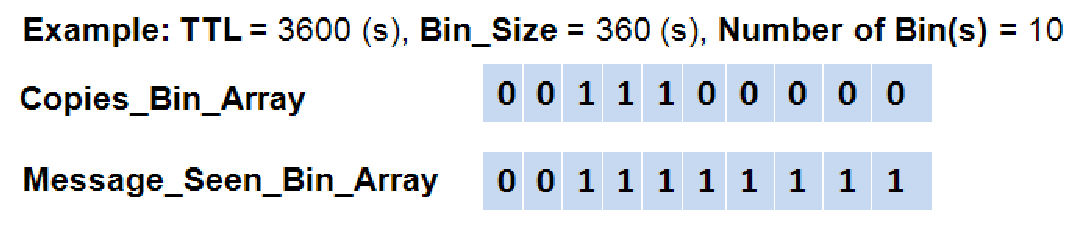
\includegraphics[width=2.5in,height=0.7in]{Chapitre3/Bin_Array.eps}
\caption{Example of Bin arrays}
\label{BA}
\end{figure}

\begin{figure}[!h]
\centering
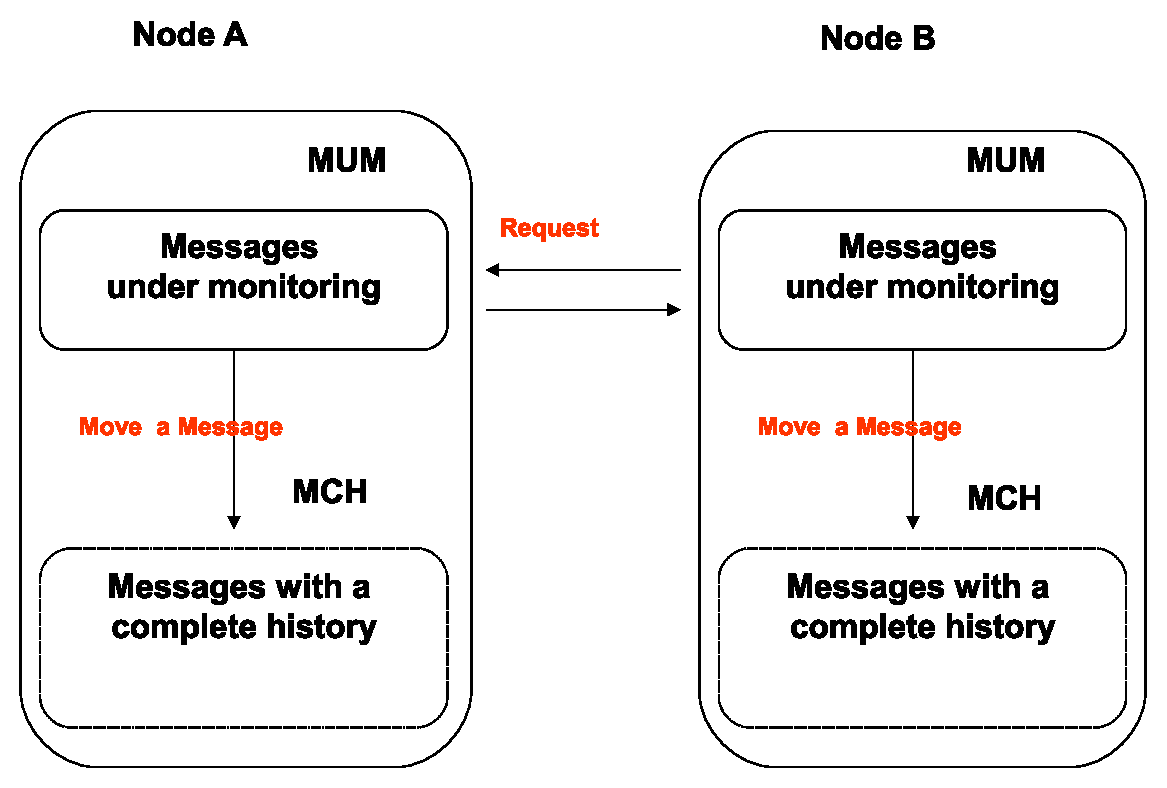
\includegraphics[width=2.5in,height=1.6in]{Chapitre3/StatisticsExchanging.eps}
\caption{Statistics Exchange and Maintenance.}
\label{SE}
\end{figure}

\subsection{Performance Tradeoffs of Statistics Collection}
\label{PENHCM}

We have presented a number of optimizations to (considerably) reduce the amount of metadata stored and the amount of signalling overhead. Here, we explore the trade-off between the signalling overhead, its impact on performance, and the dynamicity of a given scenario. Our goal is to identify operation points where the amount of signalling overhead is such that it interferes minimally with data transmission, while at the same time it suffices to ensure timely convergence of the required utility metrics per message. We will consider throughout the random waypoint simulation scenario described in Section~\ref{sec:sims:DR}. We have observed similar behaviour for the trace-based scenarios.

\textbf{Amount of Signalling Overhead per Contact:} We start by studying the effect of varying the size of the \emph{MUM} buffer (number of messages under monitoring) on the average size of exchanged statistics per-meeting. Figure~\ref{StatOverhead} compares the average size of statistics exchanged during a meeting between two nodes for three different sizes of the \emph{MUM} buffer (20, 50 and 80), as well as for the basic epidemic statistics exchange method (i.e. unlimited MUM). We vary the number of sources in order to cover different congestions regimes.

Our first observation is that increasing the traffic load (and thus the amount of congestion) results in decreasing the average amount of statistics exchanged per-meeting (except for the MUM size of 20 messages). This might be slightly counterintuitive, since a higher traffic load implies more messages to keep track of. However, note that a higher congestion level also implies that much fewer copies per message will co-exist at any time (and new versions are less frequently created). As a result, much less metadata per message is maintained and exchanged, resulting in a downward trend. In the case of a MUM size of $20$, it seems that these two effects balance each other out. In any case, the key property here is that, in contrast with the flooding-based method of~\cite{Levine:Sigcomm07}, \emph{our distributed collection method scales well, not increasing the amount of signalling overhead during high congestion.}

A second observation is that, using our statistics collection method, a node can reduce the amount of signalling overhead per meeting up to an order of magnitude (e.g. for MUM = 20), compared to the unlimited MUM case, even in this relatively small scenario of $70$ nodes. (Note also that, the plot shown for the epidemic case, already implements the binning and versioning optimizations of Section~\ref{NetworkHistoryModel}).)

\begin{figure}[!h]
\centering
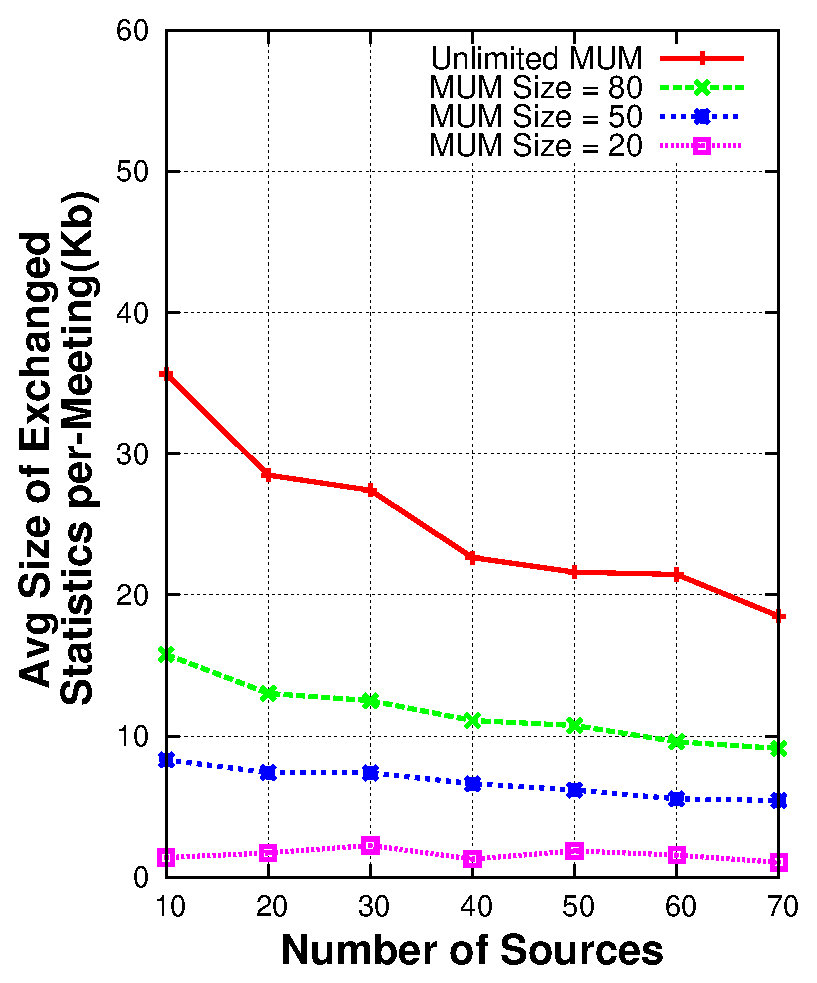
\includegraphics[width=3in,height=2.2in]{Chapitre3/fig7.eps}
\caption{Signalling overhead (per contact) resulting from HBSD statistics collection.}
\label{StatOverhead}
\end{figure}

Finally, we plot in Figure~\ref{PMED} the average size of exchanged (non-signalling) data per-meeting. We can observe that increasing the size of the \emph{MUM} buffer results in a slight decrease of the data exchanged. This is due to the priority we give to statistics exchange during a contact. We note also that this effect becomes less pronounced when congestion increases (in line with Figure~\ref{StatOverhead}). Finally, in the scenario considered, we can observe that, for MUM sizes less than $50$, signalling does not interfere with data transmissions (remember that packet size is 5KB). This suggests that, in this scenario, a MUM size of 50 messages represents a good choice with respect to the resulting signalling overhead. In practice, a node could find this value online, by dynamically adjusting its MUM size and comparing the resulting signalling overhead with average data transfer. It is beyond the scope of this paper to propose such an algorithm. Instead, we are interested in exposing the various tradeoffs and choices involved in efficient distributed estimation of statistics. Towards this goal, we explore next the effect of the MUM sizes considered on the performance of our HBSD algorithm.


\begin{figure}[!h]
\centering
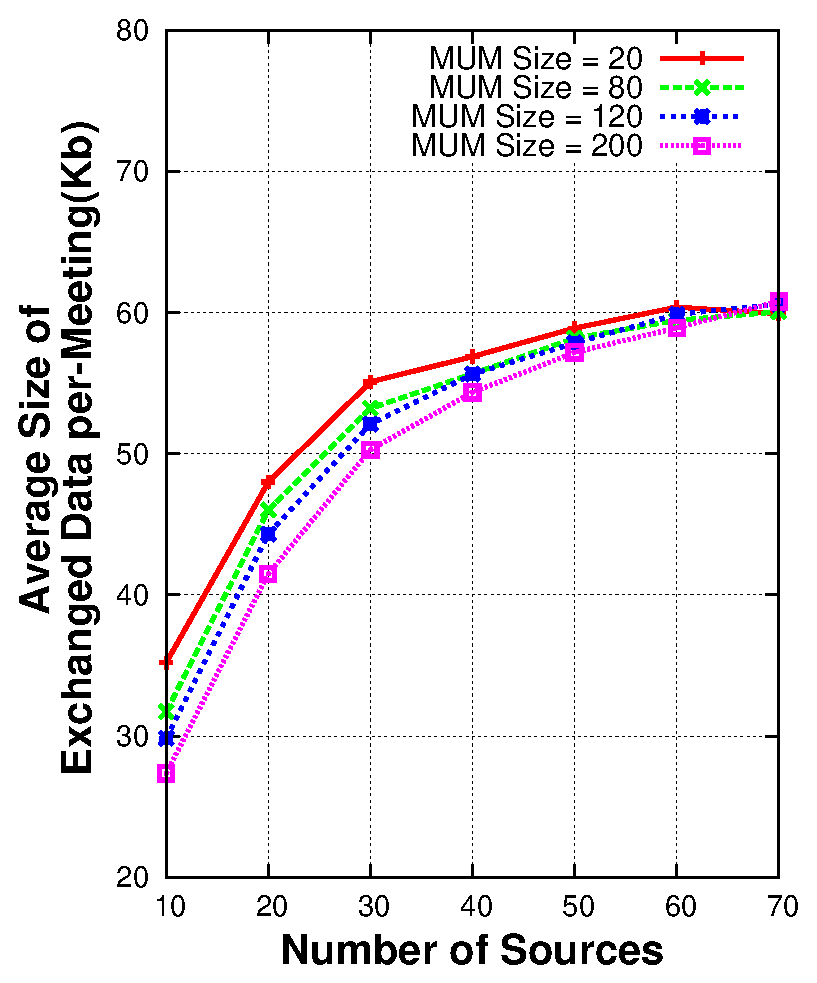
\includegraphics[width=3in,height=2.2in]{Chapitre3/fig8.eps}
\caption{Average size of exchanged (non-signalling) data per contact.}
\label{PMED}
\end{figure}

\textbf{Convergence of Utilities and Performance of the HBSD Policy :} In this last part, we fix the number of sources to $50$ and we look at the impact of the size of the \emph{MUM} buffer on (i) the time it takes the HBSD delivery rate utility to converge, and (ii) its accuracy. We use the \emph{mean relative square error} to measure the accuracy of the HBSD delivery rate utility, defined as follows:

\begin{eqnarray*}
\frac{1}{\# Bins}* \sum_{Bins}^{}\frac{(A-B)^2}{B^2},
\end{eqnarray*}

where, for each \emph{bin}, $A$ is the estimated utility value of Eq. (\ref{HBSD-DR-U}) (calculated using the approximate values of $m$ and $n$, collected with the method described previously) and $B$ is the utility value calculated using the real values of $m$ and $n$.

\begin{figure}[!h]
\centering
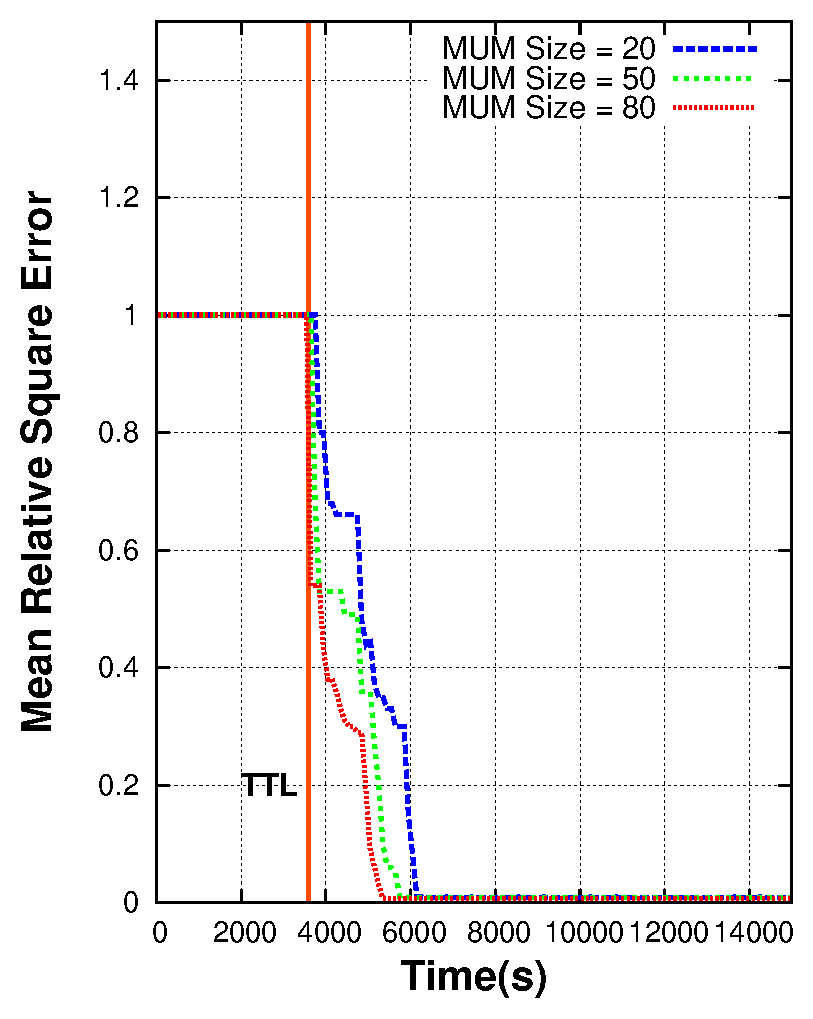
\includegraphics[width=3in,height=2.2in]{Chapitre3/fig9.eps}
\caption{Mean relative square errors for HBSD delivery rate utility.}
\label{DR-RE}
\end{figure}

Figure~\ref{DR-RE} plots the \emph{mean relative square errors} for the HBSD delivery rate utility, as a function of time. We can observe that, increasing the size of the \emph{MUM} buffer results in faster reduction of the \emph{mean relative square error} function. With a \emph{MUM} buffer of $80$ messages, the delivery rate utility estimate converges $800$ seconds faster than using an \emph{MUM} buffer of $20$ messages. Indeed, the more messages a node tracks in parallel, the faster it can collect a working history of past messages that it can use to calculate utilities for new messages considered for drop or transmission. We observe also that all plots converge to the same very small error value~\footnote{We speculate that this remaining error might be due to slightly underestimating m and n, as explained earlier.}. Note also that it is not the absolute value of the utility function (during different time bins) that we care about, but rather the \emph{shape} of this function, whether it is increasing or decreasing, and the relative utility values. (We will look into the shape of this function at different congestion regimes in the next section.)

In fact, we are more interested in the end performance of our HBSD, as a function of how ``aggressively'' nodes collect message history. In Figures~\ref{HBSD-AVG-DR-MUM} and~\ref{HBSD-AVG-DD-MUM}, we plot the delivery rate and delay of HBSD, respectively, for different MUM sizes. These results correspond to the scenario described in Section~\ref{sec:sims:DR}, where we have a fixed number of CBR sources. As is evident from these figures, regardless of the size of the \emph{MUM} buffer sizes, nodes eventually gather enough past message history to ensure an accurate estimation of per message utilities, and a close-to-optimal performance. In such scenarios, where traffic intensity is relatively stable, even a rather small MUM size (i.e. very low sampling rate) suffices to achieve good performance. This is not necessarily the case when traffic load experiences significant fluctuations (e.g. due to new popular content appearing in the network).

\begin{figure}[!h]
  \begin{center}
    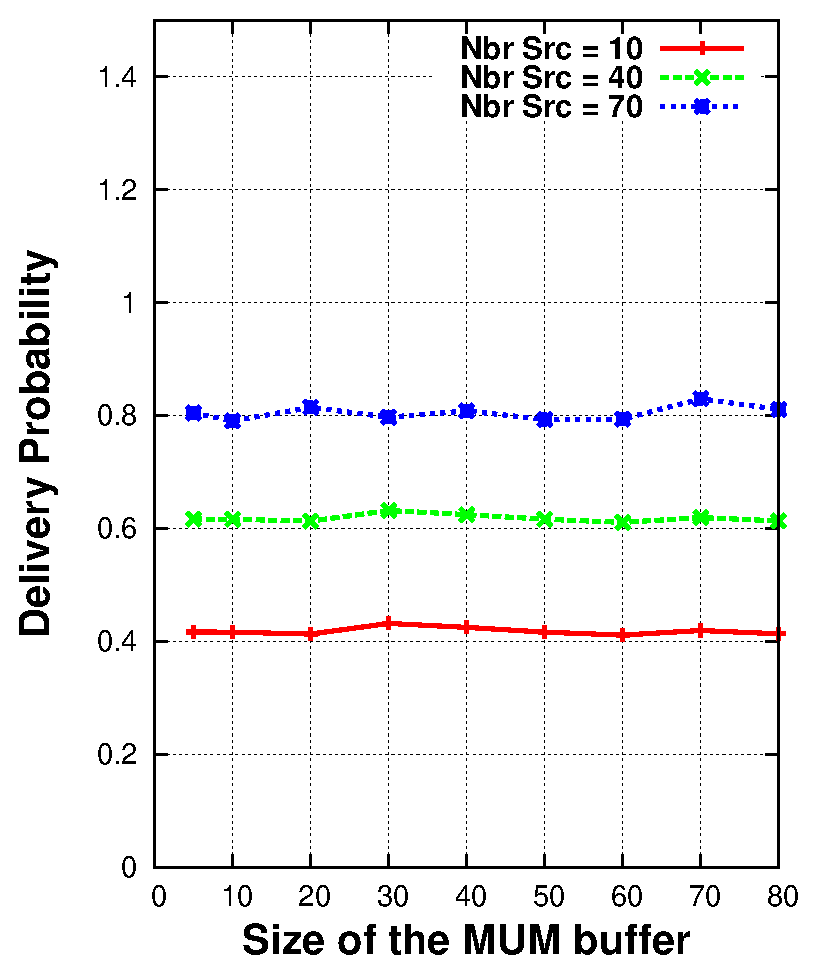
\includegraphics[width=3in,height=2.2in]{Chapitre3/fig13.eps}
  \end{center}
  \caption{Delivery Probability for HBSD with statistics collection (static traffic load).}
  \label{HBSD-AVG-DR-MUM}
\end{figure}

\begin{figure}[!h]
  \begin{center}
    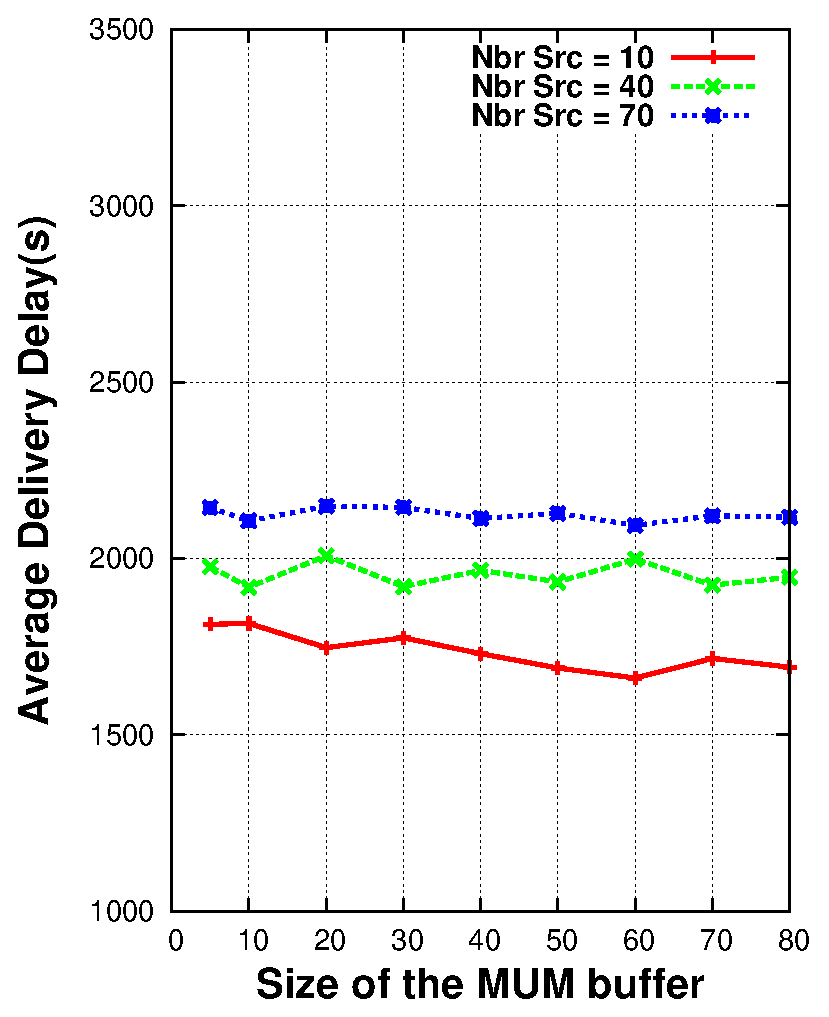
\includegraphics[width=3in,height=2.2in]{Chapitre3/fig14.eps}
  \end{center}
  \caption{Deliver Delay for HBSD with statistics collection (static traffic load).}
  \label{HBSD-AVG-DD-MUM}
\end{figure}

When the offered traffic load changes frequently (or node churn is high, e.g. experiencing ``flash crowds''), convergence speed becomes important. The bigger the \emph{MUM} buffer the faster our HBSD policy react to changing congestion levels. We illustrate this with the following experiment. We maintain the same simulation scenario, but we vary the number of CBR sources among each two consecutive TTL(s), from $10$ to $70$ sources (i.e. the first and second TTL window we have $10$ sources, the third and fourth window $70$ sources, etc. --- this is close to a \emph{worst case} scenario, as there is a sevenfold increase in traffic intensity within a time window barely higher than a TTL, which is the minimum required interval to collect any statistics). Furthermore, to ensure nodes use non-obsolete statistics towards calculating utilities, we force nodes to apply a \emph{sliding window} of one \emph{TTL} to the messages with complete history stored in the \emph{MCH} buffer, and to delete messages out of this \emph{sliding window}\footnote{A running average could be used for smoother performance. We only care here to demonstrate the effect of dynamic traffic loads.}

Figures~\ref{HBSD-AVG-DR-DYNAMIC} and~\ref{HBSD-AVG-DD-DYNAMIC} again plot the HBSD policy delivery rate and delay, respectively, as a function of MUM buffer size. Unlike the constant load case, it is easy to see there that, increasing the size of the \emph{MUM} buffer, results in considerable performance improvement. Nevertheless, even in this rather dynamic scenario, nodes manage to keep up and produce good utility estimates, with only a modest increase on the amount of signalling overhead required.

\begin{figure}[!h]
  \begin{center}
    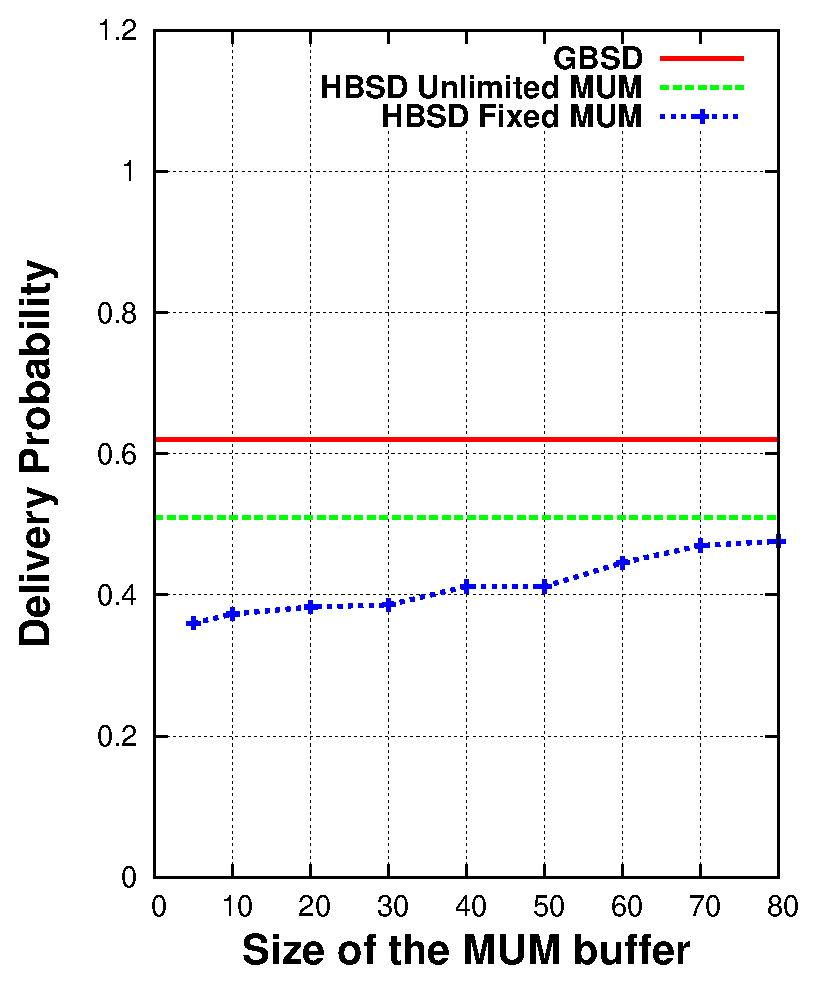
\includegraphics[width=3in,height=2.2in]{Chapitre3/fig11.eps}
  \end{center}
  \caption{Deliver Probability for HBSD with statistics collection (dynamic traffic load).}
  \label{HBSD-AVG-DR-DYNAMIC}
\end{figure}

\begin{figure}[!h]
  \begin{center}
    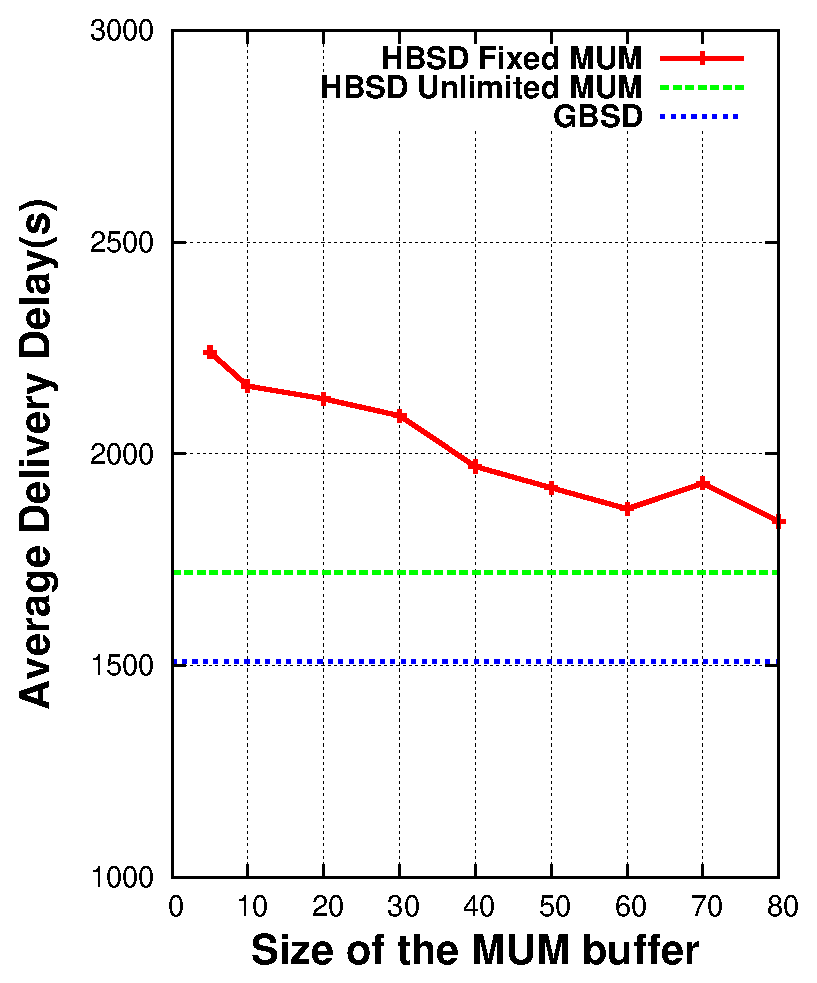
\includegraphics[width=3in,height=2.2in]{Chapitre3/fig12.eps}
  \end{center}
  \caption{Deliver Delay for HBSD with statistics collection (dynamic traffic load).}
  \label{HBSD-AVG-DD-DYNAMIC}
\end{figure}


\section{Distribution of HBSD Utilities}
\label{sec:HBSDUtilitiesDistributions}

We have described how to efficiently collect the necessary statistics in practice, and derive good estimates for the HBSD utility distribution during the lifetime of a message. In this last section, we turn our attention to the utility distributions themselves. First, we are interested whether the resulting distributions for HBSD delivery rate and delivery delay utilities react differently to different congestion levels, that is, if the priority given to messages of different ages shifts based on the offered load. Furthermore, we are interested whether the resulting utility shape (and respective optimal policy) could be approximated by simple(r) policies, in some congestion regimes.

We consider again the simulation scenario used in Section~\ref{sec:sims:DR} and Section~\ref{PENHCM}. First, we fix the number of sources to $50$, corresponding to a \emph{high congestion regime}. In Figure~\ref{HBSD-DR-HCN} and Figure~\ref{HBSD-DD-HCN}, we plot the distribution of the HBSD delivery rate and delivery delay utilities described in Sections~\ref{sec:learning:EDR} and~\ref{sec:learning:EDD}. It is evident there that the optimal utility distribution has a non-trivial shape for both optimization metrics, resulting in a complex optimal scheduling and drop policy. This also helps explain why simple drop and scheduling policies (e.g. Drop Youngest or Oldest Message, DropTail, FIFO or LIFO scheduling, etc.), considered in earlier work~\cite{Towsley:Epidemic, KrifaBS08} lead to incorrect decisions during congestion and perform worse than the GBSD and HBSD policies~\cite{KrifaBS08}.

\begin{figure}[!h]
  \begin{center}
    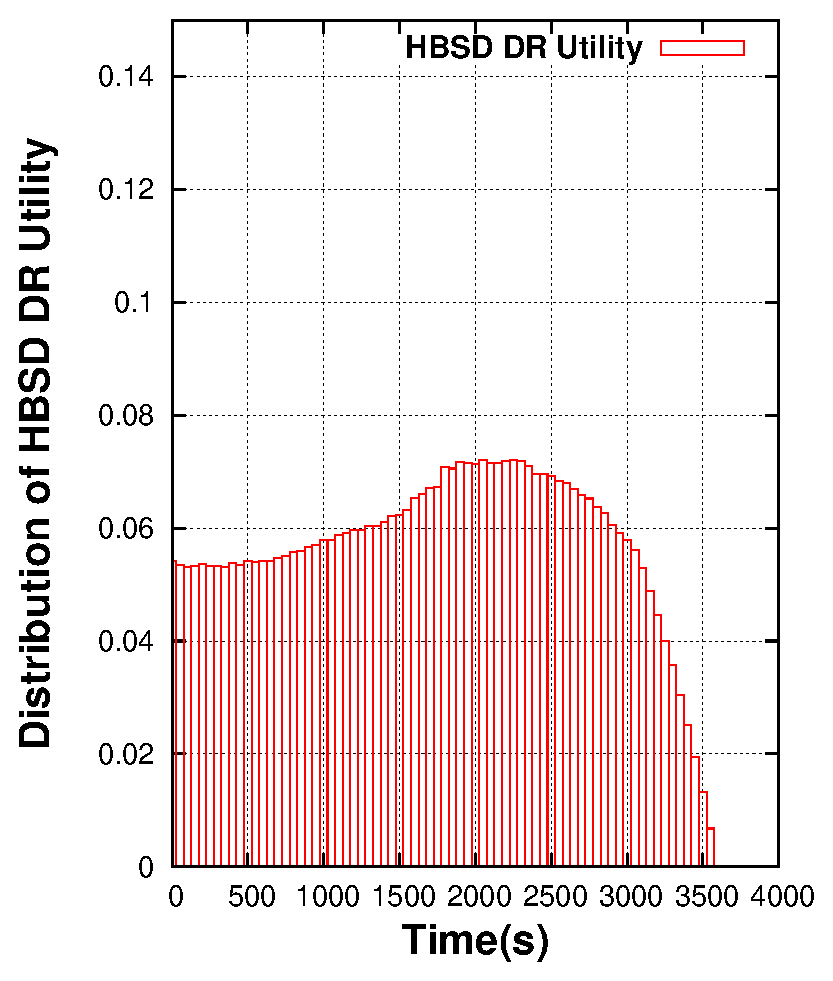
\includegraphics[width=3in,height=2.2in]{Chapitre3/fig18.eps}
  \end{center}
  \caption{Distribution of HBSD DR utility in a congested network.}
  \label{HBSD-DR-HCN}
\end{figure}

\begin{figure}[!h]
  \begin{center}
    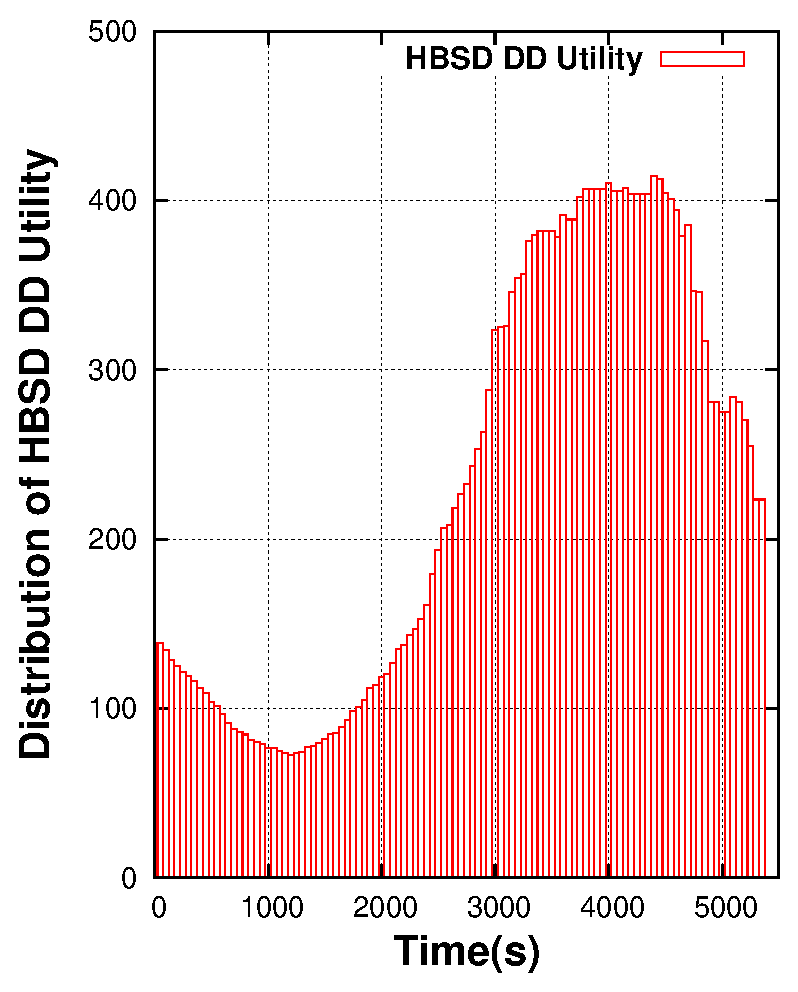
\includegraphics[width=3in,height=2.2in]{Chapitre3/fig16.eps}
  \end{center}
  \caption{Distribution of HBSD DD utility in a congested network.}
  \label{HBSD-DD-HCN}
\end{figure}

Next, we consider a scenario with low congestion. We reduce the number of sources to $15$, keep the buffer size of $20$ messages, but we also decrease the CBR rate of sources from
$10$ to $2$ messages/TTL. In Figures~\ref{HBSD-DR-LCN} and~\ref{HBSD-DD-LCN}, we plot the distribution of the HBSD delivery rate and delivery delay utilities, respectively, for this low congestion scenario. Surprisingly, our HBSD policy behaves very differently now, with both utility functions decaying monotonically as a function of time (albeit not at constant rate). This suggests that the optimal policy in low congestion regimes could be approximated by the simpler ``Drop Oldest Message'' (or schedule younger messages first) policy, which does not require any signalling and statistics collection between nodes.

To test this, in Tables~\ref{DO-HBSD-C} and~\ref{DO-HBSD-LC}, we compare the performance of the HBSD policy against a simple combination of ``Drop Oldest Message'' (for Buffer Management) and ``Transmit Youngest Message First'' (for Scheduling during a contact). We observe, that in the low congestion regime (Tables~\ref{DO-HBSD-LC}) the two policies indeed have similar performance (4\% and 5\% difference in delivery rate and delivery delay, respectively). However, in the case of a congested network (Table~\ref{DO-HBSD-C}), HBSD clearly outperforms the simple policy combination.

We can look more carefully at Figures~\ref{HBSD-DR-HCN} and~\ref{HBSD-DD-HCN}, to understand what is happening in high congestion regimes. The number of copies per message created at steady state depends on the total number of messages co-existing at any time instant, and the aggregate buffer capacity. When too many messages exist in the network (for the provided buffer space per node), uniformly assigning the available messages to the existing buffers (which is what a random drop and scheduling policy would do), would imply that every message can have only a few copies created. Specifically, for congestion higher than some level, the average number of copies per message allowed is so low that most messages cannot reach their destination during their TTL (this depends only on the number of copies and mobility model). \emph{Uniformly assigning resources between nodes is no more optimal}. Instead, to ensure that at least some messages can be delivered on time, the optimal policy gives higher priority to older messages that have managed to survive long enough (and have probably created enough copies), and ``kills'' some of the new ones being generated. This is evident by the values assigned at different bins (especially in the delivery delay case). In other words, when congestion is excessive \emph{our policy performs an indirect admission control function.}

Contrary to this, when the offered load is low enough to ensure that all messages can on average create enough copies to ensure delivery, the optimal policy simply performs a fair (i.e. equal) distribution of resources (ensured by the utility functions of Figures~\ref{HBSD-DR-LCN} and~\ref{HBSD-DD-LCN}).

\begin{table}[!h]
\renewcommand{\arraystretch}{1.1}
\caption{HBSD vs. Schedule Younger First\textbackslash Drop-Oldest in a congested network.}
\centering
\footnotesize
\begin{tabular}{|p{1.8cm}||p{2cm}||p{6cm}|}
\hline
\bfseries Policies: & HBSD & Schedule Younger First\textbackslash Drop-Oldest\\
\hline\hline
D. Rate(\%):&54&29\\
\hline\hline
D. Delay(s):&1967&3443\\
\hline
\end{tabular}
\label{DO-HBSD-C}
\end{table}

\begin{figure}[!h]
  \begin{center}
    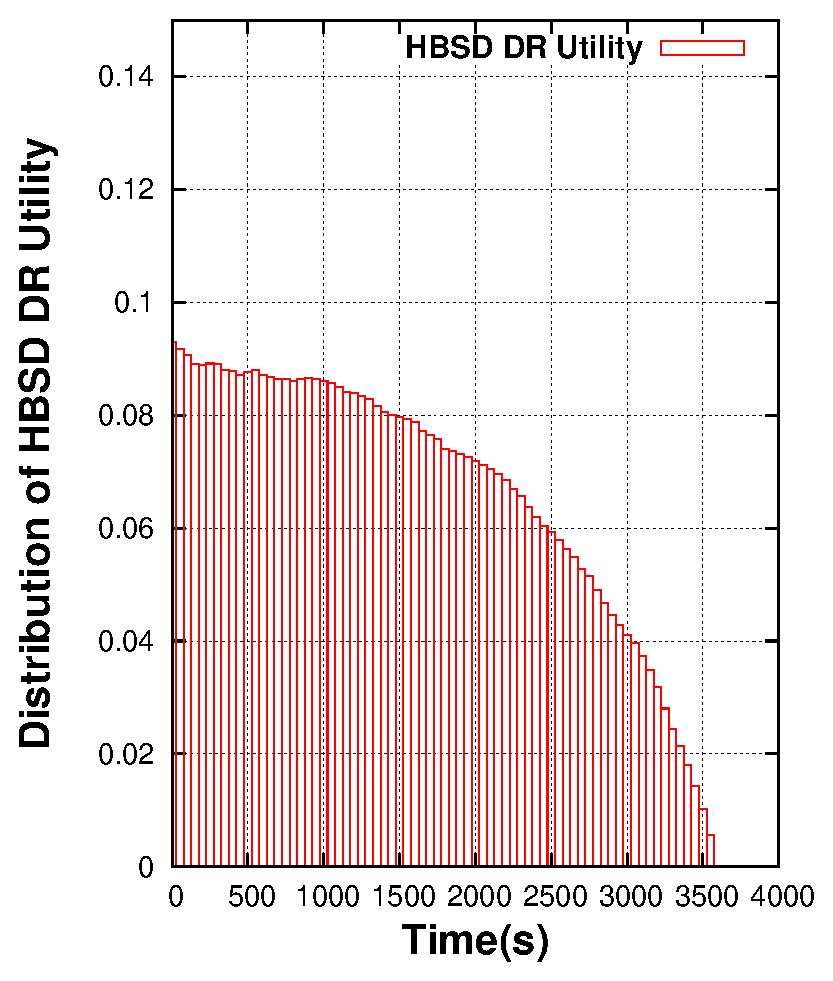
\includegraphics[width=3in,height=2.2in]{Chapitre3/fig17.eps}
  \end{center}
  \caption{Distribution of HBSD DR utility in a low congested network.}
  \label{HBSD-DR-LCN}
\end{figure}

\begin{figure}[!h]
  \begin{center}
    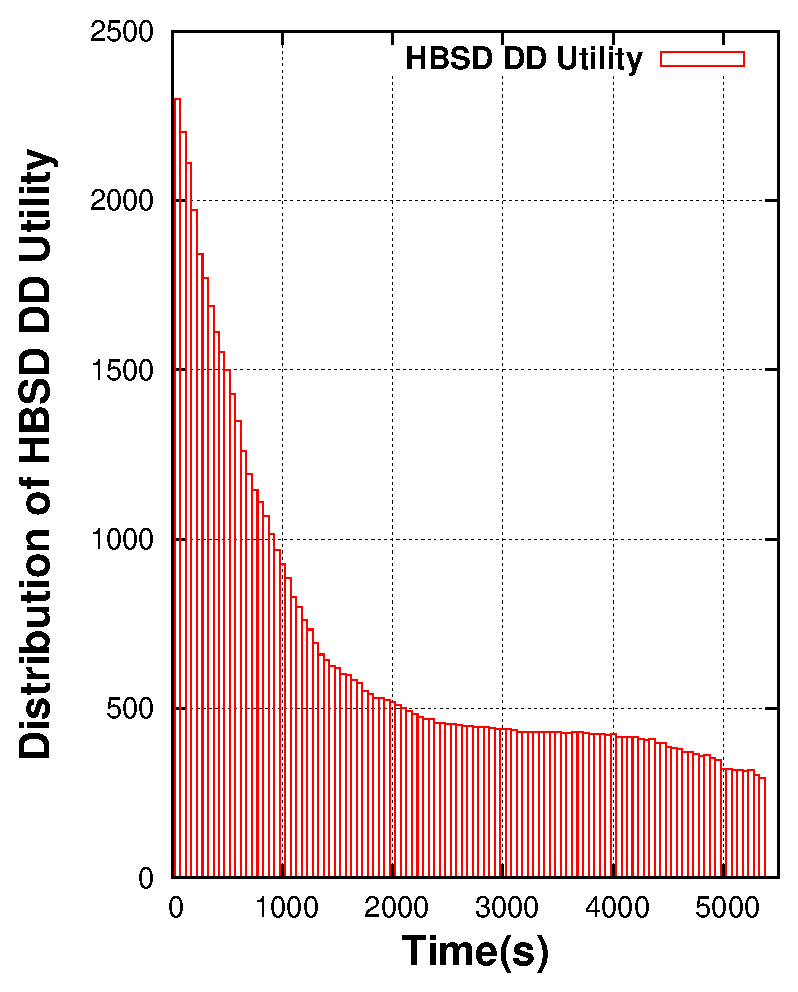
\includegraphics[width=3in,height=2.2in]{Chapitre3/fig15.eps}
  \end{center}
  \caption{Distribution of HBSD DD utility in a low congested network.}
  \label{HBSD-DD-LCN}
\end{figure}

\begin{table}[!h]
\renewcommand{\arraystretch}{1.1}
\caption{HBSD vs Schedule Younger First\textbackslash Drop-Oldest in a low congested network.}
\centering
\footnotesize
\begin{tabular}{|p{1.8cm}||p{2cm}||p{6cm}|}
\hline
\bfseries Policies: & HBSD & Schedule Younger First\textbackslash Drop-Oldest\\
\hline\hline
D. Rate(\%):&87&83\\
\hline\hline
D. Delay(s):&1530&1618\\
\hline
\end{tabular}
\label{DO-HBSD-LC}
\end{table}

The above findings suggest that it would be quite useful to find a generic way to signal the congestion level and identify the threshold based on which nodes can decide to either activate our HBSD scheme or just use a simple Drop/Scheduling policy. Suspending a complex Drop/Scheduling mechanism and its underlying statistics collection and maintenance methods, whenever not needed, can help nodes save an important amount of resources (e.g. energy), while maintaining the same end performance. Finally, we believe that the indirect signalling provided by the behaviour of the utility function during congestion, could provide the basis for an end-to-end flow control mechanism, a problem remaining largely not addressed in the DTN context.



\section{Summary and Open Issues}
\chapter{HBSD: Implementation on top of the DTN2 reference architecture}
\label{chapter:HBSD}
\minitoc

We have implemented the HBSD framework for the Delay-Tolerant Networking Research Group's DTN reference implementation (DTN2). 
In our DTN2 implementation of HBSD, users can tune the configuration and choose either to maximise the
delivery probability or to minimise the delivery delay for all DTN2 bundles. HBSD executes as an external DTN2 router, using DTN2's XML-based External Router Interface. HBSD is implemented in C++. 

This Chapter provides an overview of the implementation of HBSD for DTN2. We start by describing shortly the DTN2 architecture, we detail the DTN2 external router interface operation then we describe the implementation of the HBSD external router.

\section{DTN2 Platform Overview}
\label{DTN2}

The goal of the Delay-Tolerant Networking Research Group's DTN2  implementation is to clearly embody the components of the DTN architecture, while also providing a robust and flexible software framework for experimentation, extension, and real-world deployment.

Figure~\ref{DTN2-Arch} is a block diagram enumerating the major components of the DTN2 Bundle (application specified data 
unit) forwarding system. As can be seen from the diagram, the bundle router module represents the most central component of the implementation; in general, it requires the most detailed information regarding the state of the system upon which to base routing decisions. Decisions made by the router are passed as a set of instructions (actions) to the forwarder which is responsible for executing the actions. This separation between policy and function allows for easy extension, modification, and
replacement of the potentially complex router module. 

\begin{figure}[!h]
\centering
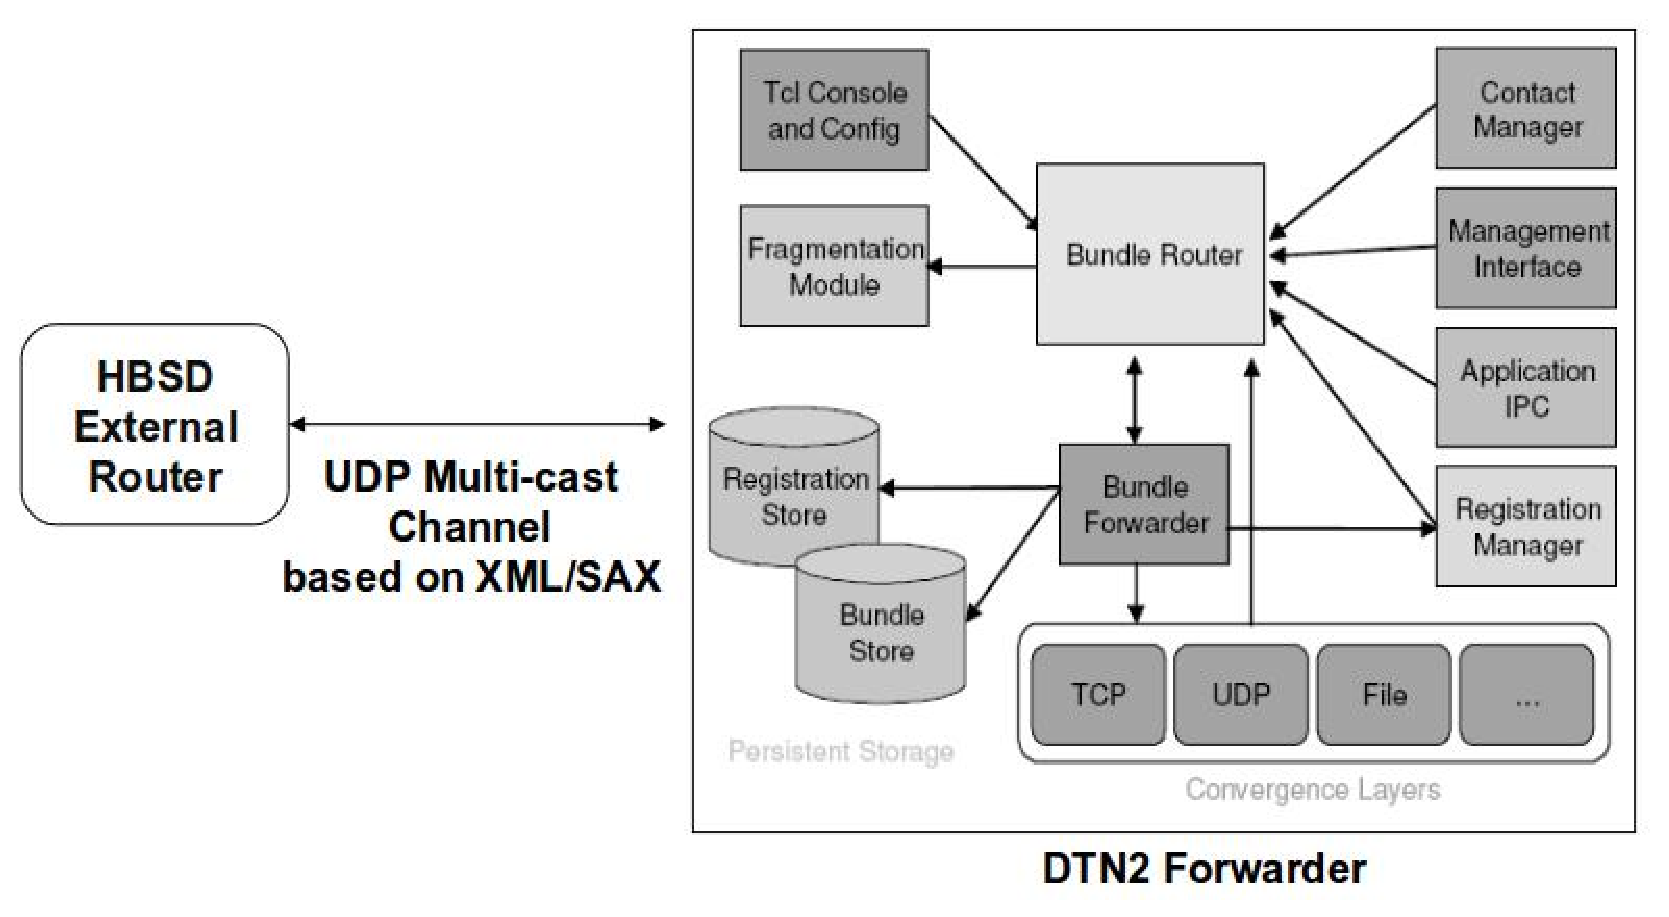
\includegraphics[width=5in,height=3in]{Chapitre4/HBSD-DTN2.eps}
\caption{DTN2 Architecture}
\label{DTN2-Arch}
\end{figure}

The DTN2 architecture provides also a set of generic external interfaces that enables third-party developers to implement plug-in modules without having to rewrite or understand the internal workings of the DTN2 reference implementation. Plug-in modules are stand-alone processes designed to work in collaboration with DTN.
The External Router Interface is the first DTN external interface designed to move bundle forwarding decisions to an external process or processes. Benefits of this interface include: \emph{(i)} classified and proprietary bundle routing algorithms are protected \emph{(ii)} external routers may be written in any programming language (XML based interface).
\emph{(iii)} prototyping of new bundle routing algorithms is streamlined and \emph{(iiii)} routing algorithms may be added and removed at runtime.

\subsection{Message Processing Modules}

\paragraph{Bundle Router and Bundle Forwarder} 
The router component implements all the route selection and scheduling policy decision making. It takes as input a large variety of events that could potentially affect
routing decisions and issues encoded instructions that are passed to the bundle forwarder, which is in turn charged with the responsibility to execute them. The forwarder executes the router's decisions by interacting with the Convergence Layers, Registrations, and the Persistent Store. The separation of router from forwarder represents an instance of separating policy from mechanism. Also, since there is different varieties of possible routing policies, separating the calculation of instructions from their execution helps to isolate the routing code from changes in the other internal APIs.

\paragraph{Convergence Layers}
Convergence Layers are the adapters between the DTN bundling protocols and various underlying transports,
similar to drivers within an operating system. At the most basic level, they perform basic data plane functions: a
particular layer must be able to transmit and receive bundles over a single hop (in the overlay topology). In some
cases they also process signaling information required by the bundle router (e.g. such as failed connections and
restarts). Convergence Layers are discussed in more detail in the following section.

\paragraph{Persistent Store}
Persistent storage is used to hold the contents of bundles during the store-and-forward process. This module provides a common abstraction for persistence storage which enables
the use of a wide variety of storage methods for holding in-transit bundles. This allows a particular system instance to select (at runtime) to use either a relational
database model or a simple file model.

\paragraph{Fragmentation Module}
The fragmentation module is responsible for fragmenting and reassembling bundle fragments. In DTN, fragmentation is used in routing both proactively when a large
message is to be moved over a contact of smaller known finite volume as well as reactively when a data 
transfer fails unexpectedly. This module is able to signal the bundle router when all the fragments of a subject bundle have
been received.

\subsection{Management Modules}

\paragraph{Contact Manager}
The Contact Manager is responsible for keeping track of which links are currently available, any historical information regarding their connectivity or performance,
and any known future schedules of when connectivity may be available. The primary task of the contact manager is to
transform the information learned about contacts from environment-specific mechanisms into abstract contact descriptions that can be used by the bundle router.

\paragraph{Management Interface}
The management interface is used to signal the bundle router about any special policy constraints or preferences
that may affect its data routing decisions. It is implemented as a generic interprocess communication capability so that multiple applications or processes may be
supported. For example, this hook could be used to signal the router to scan for potential contacts when a WiFi link detects a hotspot.

\paragraph{Console / Config}
The console/configuration module provides a command line interface and an event loop for testing and debugging of the implementation, as well as a structured method
to set initial configuration options. 

\subsection{Application Support Module}

\paragraph{Application IPC / Registration Module}

DTN applications are written to use a thin library that communicates with the router via an inter-process communication channel. Most of this interaction relates to
sending and receiving application messages and manipulating message demultiplexing bindings.

\section{DTN2 External Router Interface Operation}

Before diving into the details of HBSD implemantation, this section discusses the overall design and operation of the DTN2 external router interface. When compiled, the DTN2 produces one multi-threaded executable, a DTN daemon. This daemon is a complete DTN node; it accepts bundles from a number of built-in convergence layers, provides persistent bundle storage, delivers bundles to local DTN applications, selects routes using built-in routing logic, and forwards bundles to peer DTN nodes. A forwarder is a DTN daemon as described above, but in our case, one that depends on external routing processes to make bundle routing decisions on its behalf.

The forwarder communicates with external routing processes with an XML-based messaging protocol using a well-known IPv4 multicast address and UDP port on local or remote hosts. Before forwarders and external routers can communicate, they each must join the all-routers multicast group (224.0.0.2) and bind to a well-known UDP port. Forwarders are not aware if zero, one, or more external routers have joined the multicast group. It is the responsibility of the system administrator to ensure router availability.

Nothing in the interface design precludes running forwarders and external routers on different hosts, however this approach is not recommended especially in wireless and/or bandwidth-constrained environments. The interface is fairly chatty, UDP is unreliable, and there is a high risk of packet loss leading to a breakdown in synchronized state. (The DTN2 external router interface is hard coded to use the loopback interface and therefore requires forwarders and external routers to reside on the same host.)

Inter-process messages are XML-based and must be valid against the external router XML schema. Interface messages are broadly divided into four categories. Event messages are issued by forwarders to indicate state changes that may be of interest to external routers. Request messages are sent by external routers to direct forwarders to perform an action (e.g. "forward the bundle with ID 56 out link tcp0"). Query and report messages are used by external routers to synchronize their state with forwarders after bootup or during failure recovery. The proper usage and interpretation of each interface message is covered in the next section.

Note that DTN2 forwarder does not authenticate external processes. The forwarder makes the assumption that (local or remote) external routers are within the same security domain. In addition, system administrators must ensure there exists one authoritative router or policy module per DTN node, or that multiple external routers are configured in a cooperative manner to correctly handle all events.


\section{HBSD Implementation Overview}

The DTN2 / HBSD architecture is very simple at the highest level. The DTN2 daemon sends multicast packets 
to be received by a local router process. These packets contain XML
data and provide notification of events, such as the creation of a link or the receipt of a bundle.
The router process, in this case HBSD, sends multicast XML messages to the DTN2 daemon requesting that
some action be taken, such as the transmission of a bundle. Note that the exchanged messages
are not to be viewed only as being conversational. For example, HBSD may request that the DTN2 daemon
transmit a bundle but it does not expect a response. If the DTN2 daemon does transmit the bundle, it will send
a multicast message about the transmission, but that message is a separate event and not a
reply to the transmit request. The implication of this is that requests to the DTN2 daemon do not have negative
acknowledgments. When DTN2 establishes a connection between two nodes, HBSD is notified and the HBSD
peers exchange meta data. This information is used to prioritize the transmission of bundles in
subsequent meetings between nodes and to decide of the bundles to be deleted in case of storage congestion. 

The exchanged meta data consist of a subset of the matrix described in Figure~\ref{Stat-Mat}. The subset is defined based on the received list of (Message\_ID, Node\_ID) entries and their associated statistics versions.


\begin{figure}[!h]
\centering
\includegraphics[width=4in,height=2in]{Chapitre4/Stat_Matrix.eps}
\caption{HBSD: matrix used to maintain network statistics}
\label{Stat-Mat}
\end{figure}

By default, when the DTN2 daemon successfully transmits a bundle it then deletes the bundle. This is
not the desired behavior; otherwise HBSD would not be able to replicate bundles on
multiple nodes. That is why it's important to set early\_deletion to false in the DTN2
configuration. The proper behavior is for dtnd to retain a copy of the bundle after
transmission.

In the case where a bundle is destined for the local node, the DTN2 daemon will automatically delete
the bundle after it has been received by the endpoint. The DTN2 daemon will then send HBSD a
bundle deletion notification.

the DTN2 daemon will delete bundles when they expire and send notifications to HBSD.
If HBSD learns of a bundle delivery acknowledgement via meta data and it is in
possession of that bundle, it will ask the DTN2 daemon to delete the bundle.
If HBSD forwards a bundle to the destination node, HBSD will request that the bundle
be deleted.

Needless to say, HBSD does not actually possess, delete or transmit bundles. This is all
performed by the DTN2 daemon, dtnd. Instead, HBSD makes decisions and informs the DTN2 daemon which
bundles are to be transmitted or deleted.


\section{Main HBSD external router building blocks}

\begin{figure}[!h]
\centering
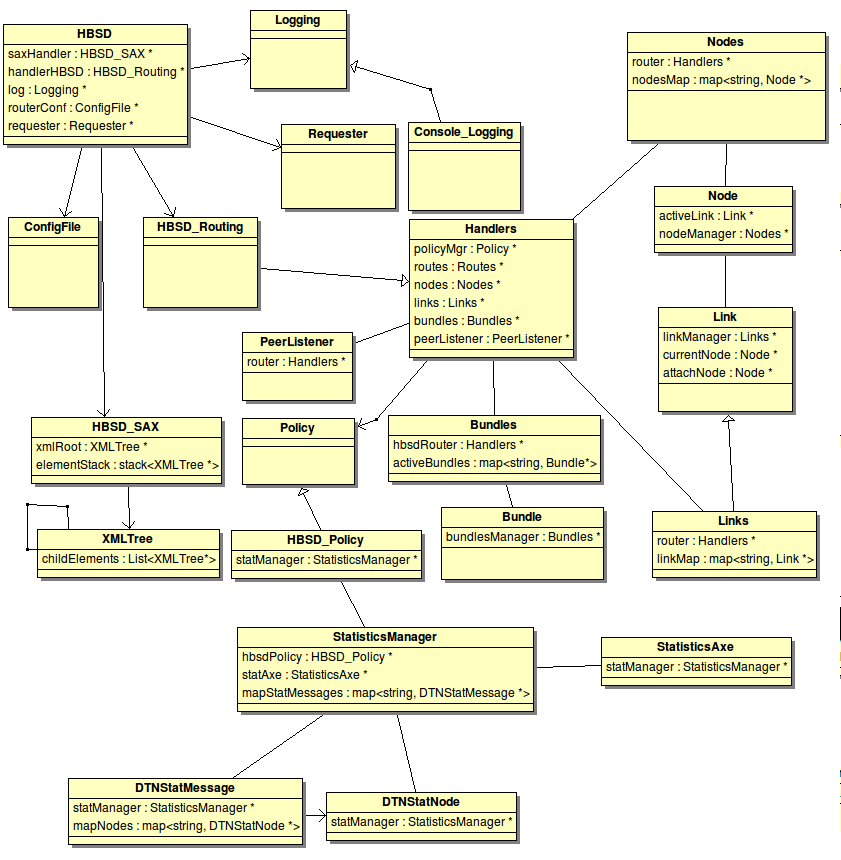
\includegraphics[width=6in,height=6in]{Chapitre4/HBSDClasses.png}
\caption{HBSD class diagram}
\label{DTN2-Arch}
\end{figure}

\paragraph{StatisticsManager class:}

This class implements the algorithms~\cite{TMC:Report} we designed to maintain network history and infer the utilities needed by HBSD either to maximize the messages average delivery probability  or to minimize their average delivery delay.  
StatisticsManager class maintains network statistics and update it each time a new metadata
bundle is received or whenever some local storage related events occur (a bundle is dropped due
to congestion, a new bundle is added,...).
StatisticsManager also calculates and returns the utility of a given bundle (given its life time)
with respect to the routing metric to optimize (either the average delivery rate or delivery
delay).

\paragraph{PeerListener Class:}

The PeerListener object exists as a thread dedicated to processing HBSD
router-specific bundles received by peer routers. DTN2 specifies that any EID
with an endpoint that begins with ext.rtr (e.g., dtn://node.dtn/ext.rtr/HBSD)
is to be destined for an external router, and it generates a specific XML
event when it receives a bundle containing the ext.rtr endpoint. When the
HBSD Routing class receives the event, it dispatches the PeerListener objects
thread to process the bundle. Specifically, the PeerListener thread extracts
the data from the bundle, deletes the bundle, and then makes a call into the
Policy Manager passing the bundles data. This is the recipient half of the
mechanism for exchanging meta data between routers. To send meta data, the
policy manager must inject a bundle into DTN2. This is done by the Policy
Manager via a method in the Requester class.


\paragraph{Requester Class:}

This is a utility class responsible for composing and sending all XML messages
to the DTN2 daemon. These classes are used throughout HBSD.
To expand on injecting a bundle, since it is fundamental to HBSD exchanging
meta data with a peer node: When the Requester injects a bundle for the router
it assigns a unique request ID to the bundle. It is up to the policy manager
to later associate the injected bundle with the request using the id. The
Requester only plays a minor role in injecting bundles: it sends the request
to DTN2 after the policy manager creates the data. But it should be noted that
injected bundles are handled differently from other bundles by HBSD. HBSD
creates a Bundle object for an injected bundle, but it does not retain
knowledge of the bundle in the Bundles class.

\paragraph{GBOF class:}
This is another utility class. In DTN2, a bundle is uniquely identified by a global 
identifier known as a GBOF (global bundle or fragment) identifier, or simply GBOF. The GBOF utility class contains static methods for manipulating the GBOF. This includes formatting the GBOF as XML as required by DTN2. It
also includes methods for creating a hash key from the values that make up the
GBOF. This hash key is used extensively and consistently throughout HBSD and
the Policy Manager for referencing uniquely a bundle.

\paragraph{HBSD Class:}

The HBSD class contains the main body of the router. This class reads the
command line arguments, loads the configuration file (if defined), starts
logging, and sets up the SAX (Simple API for XML) handler. Once initialized,
it joins the DTN2 multicast group and continuously loops receiving locally
broadcast messages from the DTN2 daemon, dtnd. When XML messages are received
from DTN2, the SAX handler is responsible for parsing the message and
dispatching the appropriate method.

\paragraph{HBSD SAX class:}

This class is invoked when HBSD receives an XML message from the DTN2 daemon.
It extends the C++ SAX DefaultHandler class. HBSD SAX parses the XML message
and calls the corresponding method in the Handlers class.

\paragraph{Handlers class:}

This is an abstract class that defines a method for each XML event message
that may be received by HBSD SAX. The HBSD Routing class is the real
implementation of the Handlers class. We use an abstract class that supplies
null methods for all XML messages. If the class that extends Handlers, i.e.
HBSD Routing, does not support an event then the empty method in Handlers in
invoked.

\paragraph{XMLTree class:}

This is a utility class. When HBSD SAX parses an XML message each element is
placed in an XMLTree object. XMLTree objects may be linked to each other to
represent the hierarchy of elements in an XML message. XMLTree objects have
methods for accessing attributes and child elements.

\paragraph{HBSD Routing class:}

The HBSD Routing class is the heart of the router, extending the methods
defined by Handlers. It is here that the XML messages sent by the DTN2 daemon,
as represented by XMLTree objects, are initially acted upon.

\paragraph{Logging class:}

This is an interface that defines the logging class used by the HBSD router.
HBSD provides one implementation of the Logging class: Console Logging. By
default, Console Logging is used though you can define which implementation to
invoke via the HBSD configuration file.

\paragraph{Console Logging class:}

This is a simple implementation of the Logging interface that outputs logging
messages to stdout. It is the default logging class

\paragraph{ConfFile class:}

This is a utility class that reads and parses the HBSD configuration file.

\paragraph{Bundles class:}

This class manages the set of individual Bundle objects.

\paragraph{Node class:}

A Node object represents a node, e.g. dtn://node.dtn. HBSD creates a Node
object whenever it learns of a node, such as when a link is established to a
node, or when a received bundle references a node.

\paragraph{Nodes class:}
This is the class that manages the set of individual Node objects.

\paragraph{Link class:}

A Link object represents a DTN2 link and an instance is created whenever DTN2
notifies HBSD that it has created a link. A Link object may become associated
with a Node object when the link is opened; a DTN2 link that is not open is
not associated with a Node. When a link is open it represents communication
with another node. HBSD will associate the Link with the corresponding Node
object, unless the Node object is already associated with another Link object.
A node will never be associated with more than one link, even if there are
multiple links open to the same node.

\paragraph{Links class:}
The Link class manages the set of individual Link objects.

\paragraph{Policy class:}
The Policy class defines the interface to be implemented by a Policy Manager.
The interface source code describes the individual methods. By default,
HBSD Policy implements this class, but other implementations can be defined
via the HBSD configuration file.

\paragraph{HBSD Policy class:}

This class is an implementation of the Policy class. It provides the HBSD
scheduling and drop algorithm, but it is also generically referred to as the
Policy Manager. There are calls into the Policy class sprinkled throughout the
router, often mirroring the XML events defined by the /etc/router.xsd schema
file. HBSD Policy largely consists of manipulating shadow data structures
dealing with bundles and nodes. The primary function of HBSD Policy is to
prioritize the delivery and replication of bundles in anticipation of the
local node coming into contact with another node. The assumption is that HBSD
will be able to replicate only a subset of its bundles on each node that it
meets, and that some of the bundles will expire before HBSD comes in contact
with the actual destination node.


\section{Configuring HBSD}

HBSD can be customized through a configuration file specified in the runtime command line.  
There must be no more that one configuration option per line in the file, and must be specified using the syntax: variable=value. The value may be double or single-quoted. Lines that begin with a hash character ($\#$) are treated as comments and ignored. Comments should not appear on the same line as a configuration value. The options defined in the following table are supported. The default values for most, if not all variables should be sufficient.

\begin{longtable}[!h]{|p{4cm}|p{1cm}|p{2cm}|p{5cm}|}
\hline
\textbf{Variable}& \textbf{Type} & \textbf{Default} & \textbf{Description} \\
\hline
routerEndpoint &  string & ext.rtr/HBS & Defines the external router's endpoint, which is typically  used to receive control 
messages from peer  instances of the router. An 
example is meta data exchanged between the 
routers. DTN2 special-cases endpoints that begin with 
"ext.rtr/". All communicating routers need to agree on the  endpoint name.\\
\hline
multicastGroup & string &  224.0.0.2 & Defines the multicast group the router is to join for  exchanging XML messages 
with the DTN2 daemon. This is defined by DTN2.\\
\hline
multicastPort & int & 8001 & Defines the multicast port  used by the DTN2 daemon. This is defined by DTN2.\\
\hline
multicastSends & bool & false & Defines the type of socket used to send requests to
dtnd. If true, use a multicast socket joined to the multicast group and a TTL of 0. If false, use a datagram socket bound to the 
loopback address. The goal is to send messages with their scope limited to the 
local system. On some systems the TTL is not honored. On other systems, not using a multicast socket does not work. \\
\hline
loopbackAddress & string & 127.0.0.1 & Address to bind to if multicastSends=false.\\
\hline
xmlSchema & string  & router.xsd& File containing the XML schema definition for the 
messages exchanged with dtnd, the DTN2 daemon. This file should be supplied by DTN2. The command line has precedence.\\
\hline
xmlValidate & bool & true & If set to false then the XML received from the daemon is 
not validated against the schema.\\
\hline
loggingClass & string & Console\_\ Logging & Allows for a user-specified logging class. The default is Console\_Logging.\\
\hline
logConfiguration & string  & & Logging configuration file. The command line has precedence. The format of the file is logging class 
specific. The command line has precedence.\\
\hline
logLevel & int  & 6& Logging level. The command line has precedence. If not specified, the default is defined by the logger. \\
\hline
terminateWithDTN & bool & true& By default HBSD terminates when dtnd indicates that it is shutting down. Set to false to override this behavior.\\
\hline
bundlesActiveCapacity & int  &384 & Initial capacity of the Map of all bundles on the system.\\
\hline
linksHashCapacity & int & 16& Initial capacity of the Map of all links.\\
\hline
nodesHashCapacity & int & 32& Initial capacity of the Map of all nodes.\\
\hline
enableHbsdOptimization & bool  & false & Says whether to enable or disable the HBSD statistics based optimization or to just run the epidemic routing protocol. \\
\hline
hbsdOptimize\ Performance & int & 0 & Selection of the optimization problem 0 means that the HBSD policy will try to manage both the buffer and links congestion in order to maximize the network average delivery rate. 1 means that the HBSD policy will try to manage both the buffer and links congestion in order to minimize the network average delivery delay. \\
\hline
numberOfNodesWithin\ TheNetwork & int & - &The approximated number of nodes in the Network.\\
\hline
useOnlineAproximated\ NumberOfNodes  & bool & true &  If set to true  then the HBSD policy will use the online approximated number of nodes instead of the user provided one (numberNodes above) .\\
\hline
binSize & int & 100&The bin size. Could be approximated by the average nodes meeting time.\\
\hline
numberOfBins & int & 36& The length of the Bins table. Should be equal to the messages TTL (total time to live) devided 
by binSize. Here we are supposing that all the generated messages have the same TTL value.\\
\hline
mumBufferCapacity & int & 50& The maximum capacity of the MUM buffer, the one holding the message under monitoring. \\
\hline
mchBufferCapacity & int & 1000 & The maximum capacity of the MCH buffer, the one holding the message with complete history. 
(Note: keep this  buffer infinite if you are sure that your network will maintain the same behaviour during time otherwise choose the correct capacity in order to track the network dinamicity.\\
\hline
useBinSizeAsAvg\ MeetingTime & bool & true& Specifies either to use the binSize as an expected average meeting time or to calculate online the average meeting time between nodes. Note that you should figure out an approximation of your network average meeting time in order to correctly trak the dinamicity of the network  through the binSize.\\
\hline
\end{longtable}

Please note that more details about how to install/run both the DTN2 daemon as well as our HBSD external router could be found in HBSD webpage~\cite{HBSDDTN2}. HBSD open source code is also available for downloading from~\cite{HBSDDTN2}. 

\section{Summary and Open Issues}


\chapter{Interest Driven Content Dissemination Architecture for Disruption Tolerant Networks}
\label{chapter:PTMP}
\minitoc

Mobile networking is quickly reaching a tipping point. While data has been a second-class customer for cellular networks until recently, the wide spread of smart phones, and the access these provide to existing and novel applications, are generating unprecedented amounts of mobile data. The capacity of current cellular infrastructures has already been pushed to the limit~\cite{ATT}. To support the increasing number of devices generating data at high rates, ISPs will inevitably be pushed towards either lowering bandwidth quotas~\cite{ATT}, adopting non flat rate plans, or deploying (expensive) next generation equipment. This has lead many researchers (and industry) to explore alternative or hybrid architectural solutions~\cite{CellOffLoading}.

To this end, direct mobile-to-mobile communication can be leveraged to harvest the large amounts of unused bandwidth between wireless devices in proximity. While multi-hop communication over mobile devices has been recently dealt with in the context of Delay Tolerant Networks (DTNs), increasing user demand for content is creating a shift in focus towards content and data centric systems (e.g. the CCN project~\cite{CCN}), in both wired and wireless Internet. As a result, a number of content dissemination systems have been recently proposed for mobile devices \emph{in the wild} to exchange content of interest in a peer-to-peer manner~\cite{TACODTN, Peoplenet, podnet07, May07wirelessopportunistic, ContentPlace, OptimalChannelChoice, SocialCast, Boldrini:2008:MDD}.

In addition to dealing with the challenging networking conditions, content sharing systems for DTNs have two main functions to perform: \emph{(i)} propagation of interests and content discovery;  \emph{(ii)} delivery of matching content (over one or more hops);
A number of architectural decisions can be made to achieve these goals, leading to publish/subscribe systems~\cite{TACODTN, Peoplenet}, query-based, broker-based~\cite{podnet07, LOCUS, May07wirelessopportunistic, ContentPlace, OptimalChannelChoice, SocialCast, Boldrini:2008:MDD}, etc. These systems aim to maximize the amount of useful content users can receive from the network. Nevertheless, distributed (or peer-to-peer) content sharing systems have one more important goal: \emph{(iii)} \emph{to ensure enough nodes collaborate to make the system interesting to participants.} This goal is often \emph{conflicting} with optimal algorithms for \emph{(i)} and \emph{(ii)}, and has been a major ``deal-breaker'' in most envisioned architectures for mobile ad hoc networks~\cite{NashEquilibria}. Mobile devices are controlled by rational people and we should expect them to behave selfishly by attempting to maximize their revenues and conserve their resources, unless cooperation is somehow incentivized and free-riders penalized.

The following ``architectural dilemma'' arises then when considering a content sharing architecture over \emph{non-altruistic} mobile devices. Nodes can choose to only store and share content they personally consume (thus somewhat mitigating selfish ``inclinations''), and new content of interest can be retrieved from encountered nodes~\cite{podnet07}. This greatly simplifies content discovery and delivery. To further protect nodes against free-riders, a tit-for-tat (TFT) mechanism could be enforced. Yet, this approach is very restrictive: content of interest can be retrieved \emph{only if the set of encountered nodes are also interested in (and carry) the requested content}.
This can lead to long delays and a \emph{suboptimal} query success rate \emph{even if TFT is not used}, if the mobility of nodes with common interests do not coincide.

To improve hit rates, nodes could use their spare resources (contact bandwidth, disk space) to collect, store, and relay additional content, not to be consumed locally~\cite{ContentPlace, SocialCast, OptimalChannelChoice, SocialCast, Boldrini:2008:MDD}. An interesting optimization problem then arises: how should the total spare bandwidth in the network be optimally allocated to available content so as to maximize the overall network hit rate? Answers include randomized or popularity-based local heuristics~\cite{May07wirelessopportunistic}, using this buffer space only for ``friends'' and social peers~\cite{ContentPlace, SocialCast, Boldrini:2008:MDD}, as well as optimal distributed algorithms~\cite{OptimalChannelChoice}. Unfortunately, none of these solutions answers \emph{why} participating nodes should collaborate implementing the policy of choice. In fact, we argue that \emph{this optimization problem needs to be turned on its head, in light of the non-altruistic nature of users.}

Throught this chapter, we propose MobiTrade, an approach that optimizes the content sharing strategy from the perspective of each individual participant, rather than that of the network. First, we argue that Tit-For-Tat (TFT) should be directly employed in order to \emph{(a)} isolate free-riders and \emph{(b)} create incentives for nodes to share their resources. TFT gives content of non-direct interest monetary value. If a node B has content that A is interested in, but A does not have something to give back, A now has the incentive to fetch something for B (perhaps from a remote node that B never encounters). B now retrieves content that would otherwise be inaccessible to it (due to its mobility pattern), and A retrieves content that is easy accessible but that it couldn't ``afford'' before. While TFT is well known both in P2P~\cite{BitHoc} and opportunistic networks~\cite{BarterDTN} communities, it does not answer itself, \emph{how mobile devices should optimally (re-)act in the presence of TFT} towards maximizing their revenues. MobiTrade answers this question by introducing a content utility framework that aims to \emph{maximize the expected future exchange value of the content inventory stored by each node}. Intuitively, the value of a piece of content to a node A should depend on \emph{(i)} how many are interested in it, \emph{(ii)} how often does A see these nodes, \emph{(iii)} how much content, interesting to A, do these nodes have, \emph{(iv)} how ``well-behaved'' are these nodes. MobiTrade uses a simply, robust utility function that implicitly captures all these features, without explicitly measuring each one, that turns each node into a \emph{merchant} fetching the content that has the highest chance to be sold (and exchanged for content of interest) to its good \emph{clients}

Summarizing, the major contributions of this work are the following:
\begin{enumerate}
    \item We formulate the optimal content sharing problem in DTNs from the perspective of non-altruistic nodes and assuming a tit-for-tat mechanism to isolate free-riders.
    \item We propose MobiTrade, a utility-based solution to this problem that predicts the (exchange) value of each piece of content and provides a customized resource allocation strategy for each node, \emph{matched} to each own interests and mobility pattern.
    \item Using a game-theoretic framework and simulations (with both real and synthetic mobility), we show that turning on the MobiTrade mechanism is an \emph{efficient} Nash equilibrium.
\end{enumerate}

To our best knowledge, this is the first content sharing system for DTNs that can both deal with rational, selfish nodes while at the same time achieving good global outcomes \emph{without explicit hard constraints on the topology and dependency of nodes}. 

The rest of this chapter is organized as follow. Section~\ref{MobiTrade-architecture} describes the MobiTrade architecture. Then, we provide a detailed simulation analysis in Section~\ref{performance-evaluation} based on both synthetic~\cite{HCMM} and real mobility traces~\cite{KAIST} and we compare MobiTrade to different content dissemination policies. Finally, we summarize our conclusions and discuss future work in Section~\ref{conclusion}.


\section{MobiTrade Architecture}
\label{MobiTrade-architecture}
\subsection{MobiTrade Data Records}
\label{content-channel-records}

In a content dissemination architecture, nodes need first to somehow express their interests for different (types of) content and advertise these interests. To this end, we borrow the concept of \emph{channels}, introduced in~\cite{May07wirelessopportunistic}. Specifically, the MobiTrade architecture relies on two data records: content and channel records (Figure~\ref{records}).

\emph{Channel Record:} A user asks for a set of contents by creating locally a channel record that encapsulates the set of keywords the user thinks they better describe the contents she is looking for. Channels can be added or deleted by the user, at any time. In contrast to the CCN model~\cite{CCN}, the channel record in MobiTrade is \emph{one-for-many} (not one-for-one). A desirable content is identified based on a match between the channel keywords and the content description (also characterized by a set of keywords). We think that such a match process is more appropriate for the communication model we are proposing, where the user might not know the exact content he is looking for, or might anyway be interested in all contents matching the description (e.g. Madonna songs, photos of Nice, sports tickets for sale). 

A lot more can be said about this channel structure (e.g. hierarchies, merging and splitting of channels, semantic content matching, etc.), but this is beyond the scope of this paper. Instead, we choose to use a simple channel structure here and focus on the algorithmic part of the system. Finally, each channel record contains a \emph{utility} entry. This is a key quantity for MobiTrade, allowing our system to optimize various important functions (scheduling, inventory management, collaboration profiling, etc.). For now, we will assume this as given, but Section~\ref{managing-channels} is devoted to how this utility is derived.

\emph{Content Record:} In addition to the content description, a content record contains a number of additional fields. First, we associate to each MobiTrade content a $TTL$ (Time to Live). By the end of this time, records can be removed. The cases requiring this $TTL$ field are many, for example someone could be interested in selling something today. To ensure devices respect this $TTL$ field, MobiTrade devices do not reward each other for expired content.

\begin{figure}[!h]
\centering
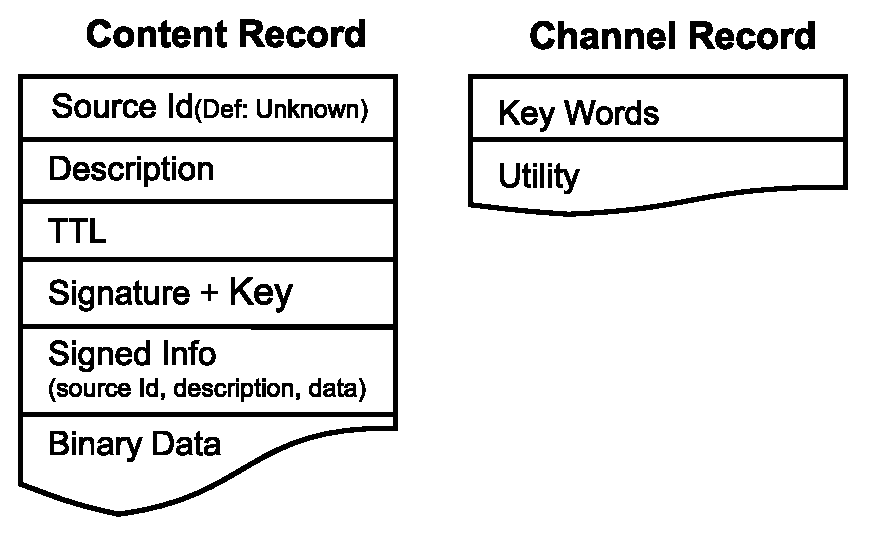
\includegraphics[width=2.5in,height=2in]{Chapitre5/ContentsInterestsRecords.eps}
\vspace{-0.1in}
\caption{MobiTrade data records and channel storage}
\label{records}
\vspace{-0.2in}
\end{figure}

Furthermore, to provide users with a full control over their privacy (i.e., the contents they publish and their center of interests), we choose to keep anonymous any generated channel record (no user or device ID are stored). Nevertheless, for contents, one still has the possibility to associate to them a \emph{canonical} source name that refers in some way to the content publisher. This field does not correspond necessarily to the user device address, but it can hold the publisher postal address or its phone number, which can be used for distinguishing between contents, feedback mechanisms on separate communication mediums or authentication purposes.

Finally, to provide for some MobiTrade security, we choose to use a CCN like \emph{content-based security} model~\cite{CCN}. With this model, protection and trust travel with the content itself, rather than being a property of the connections over which it is transmitted.
MobiTrade devices authenticate via the signature field (Figure~\ref{records}), the binding between the content source ID, its description and some parts of its data. In addition to this signature, each signed MobiTrade content carries with it the public key necessary for its verification by other devices. The signature algorithm can be selected to meet the performance requirements of that particular published data.

\subsection{MobiTrade Protocol}
\label{communication-protocol}

Communication within the MobiTrade architecture is driven by the consumers of contents. A user asks for contents by ``joining'' a channel to which these might belong, storing the respective record(s) locally on the device until it becomes out of date. Then, each time a new meeting opportunity arises with another mobile device, both devices initiate the MobiTrade communication protocol that has two main functions:
\begin{itemize}
\item (\emph{Fair Content Exchange}) to help nodes identify content of interest in their peer's inventory (buffer) and provide a set of rules to exchange such content in a \emph{fair} manner.
\item (\emph{Inventory Management}) to allow nodes to profile each exchange (\emph{learning}) and use this knowledge to improve the outcome of future interactions (\emph{prediction}).
\end{itemize}

The MobiTrade protocol is summarized in Figure~\ref{protocol}. Each device starts by sending its list of channels to the other device. Based on it, each device decides on the set of contents to forward, i.e. content in its buffer matching one of the channels requested by its peer. These contents are scheduled for transmission and passed to the \emph{Tit-For-Tat (TFT)} trading algorithm (Section~\ref{contents-trading-scheduling}) that ensures an equitable exchange.

In addition to channels the node is personally interested in, if extra space is available, it might choose to join ``foreign'' channels. Content for these channels is not stored for personal consumption, but can be used as exchange currency during the TFT phase, in order to acquire additional content of interest. This provides the incentive to nodes to act as \emph{merchants}, collecting and carrying content to be used only for trading. This also allows content to \emph{propagate efficiently across the network and between remote producer-consumer pairs, without any explicit routing mechanism}. %From the perspective of the MobiTrade protocol, own and foreign channels are equivalent.

After content starts being exchanged (one-by-one), a node receiving a content might need to perform some inventory management. First, if it already has this piece of content (or the content is expired), it will drop it\footnote{This is possible, since nodes only send to each other lists of channels and not a detailed list of contents. This is a coding trade-off that tries to avoid large amounts of meta-data being exchanged before any actual content is sent. On the other hand, it might also lead to some wasted bandwidth if lots of duplicate content is transmitted. A possible middle-ground solution to this problem could be the use of Bloom filters.}. If the content is new, and there is available buffer space for the channel this belongs to, the content is stored in the buffer. The exchange finishes once the transfer of the requested contents ends or the two devices get out of the range of each other. At this point, both devices update the set of channels they are keeping track of as well as their corresponding utilities based on the (profiled) outcome of the session (as explained in Section~\ref{managing-channels}).

\subsection{Proportional Storage and Bandwidth Allocation}
\label{buffer-management}

In a context with many nodes, various channels, and lots of multimedia content, node buffers will be operated most of the time at capacity and contact duration between nodes might not suffice to exchange all intended content. This highlights the need for efficient resource allocation algorithms. Unlike related work~\cite{ContentPlace}~\cite{May07wirelessopportunistic}, \emph{MobiTrade allocates both buffer space and contact bandwidth in an equitable way among the different channels.}

First, MobiTrade implements a mechanism of \emph{proportional soft quotas} to share available buffer space among channels. Let a node carry $N$ channels with channel utilities $U(i), i \in \{1,N\}$, and have a total buffer capacity of $B$. Then, the \emph{quota} $B(i)$ of the buffer space channel $i$ is entitled to is
\begin{eqnarray*}
B(i) = \frac{U(i)}{\sum_{i} U(i)} B.
\end{eqnarray*}
The proportion of storage allocated to a channel is proportional to its utility. Quotas are updated whenever one or more of the channel utilities change or channels are added/removed.

Based on these quotas and the amount of storage channel $i$ is \emph{currently} occupying, let $S(i)$, a node receiving a content (of $W$ bytes) for channel $i$ will perform the following actions:
\begin{itemize}
\item if $S(i) + W < B(i)$, then store the content.
\item if $S(i) + W > B(i)$ and $\sum_{i} S(i) + W < B$, then store content.
\item if $S(i) + W > B(i)$ and $\sum_{i} S(i) + W > B$, then pick the channel $j$ maximizing $\max_{j} (S(j) - B(j))$ and drop the oldest content for this channel.
\end{itemize}
Points (2) and (3) above imply that the quotas $B(i)$ are soft. Channels can exceed their share and take over free space, if any is available. However, as soon as the buffer is full, the policy pushes shares back to their just proportion.

Finally, in the presence of limited contact durations, a device cannot simply forward contents by decreasing order of the utilities of their channels since a channel can match more than one content. For example, a MobiTrade device can face a situation where many contents match a popular channel, and hence it keeps forwarding only those contents at the expense of other channels which are less popular. To remedy this, MobiTrade applies the \emph{Weighted Fair Queuing} policy which prevents starvation of channels and ensures that contents are forwarded proportionally to the utility value of the channel they match. 

As a final note, when the scheduling policy decides to forward a set of contents from the same channel, MobiTrade sends the \emph{youngest} contents first. This decision is motivated by our findings in~\cite{TMC:Report} and is complementary to the drop oldest policy applied among the contents of the same channel in case of congestion. More sophisticated policies could be also applied~\cite{TMC:Report}, but this is beyond the scope of this paper.

\begin{figure}[!h]
\centering
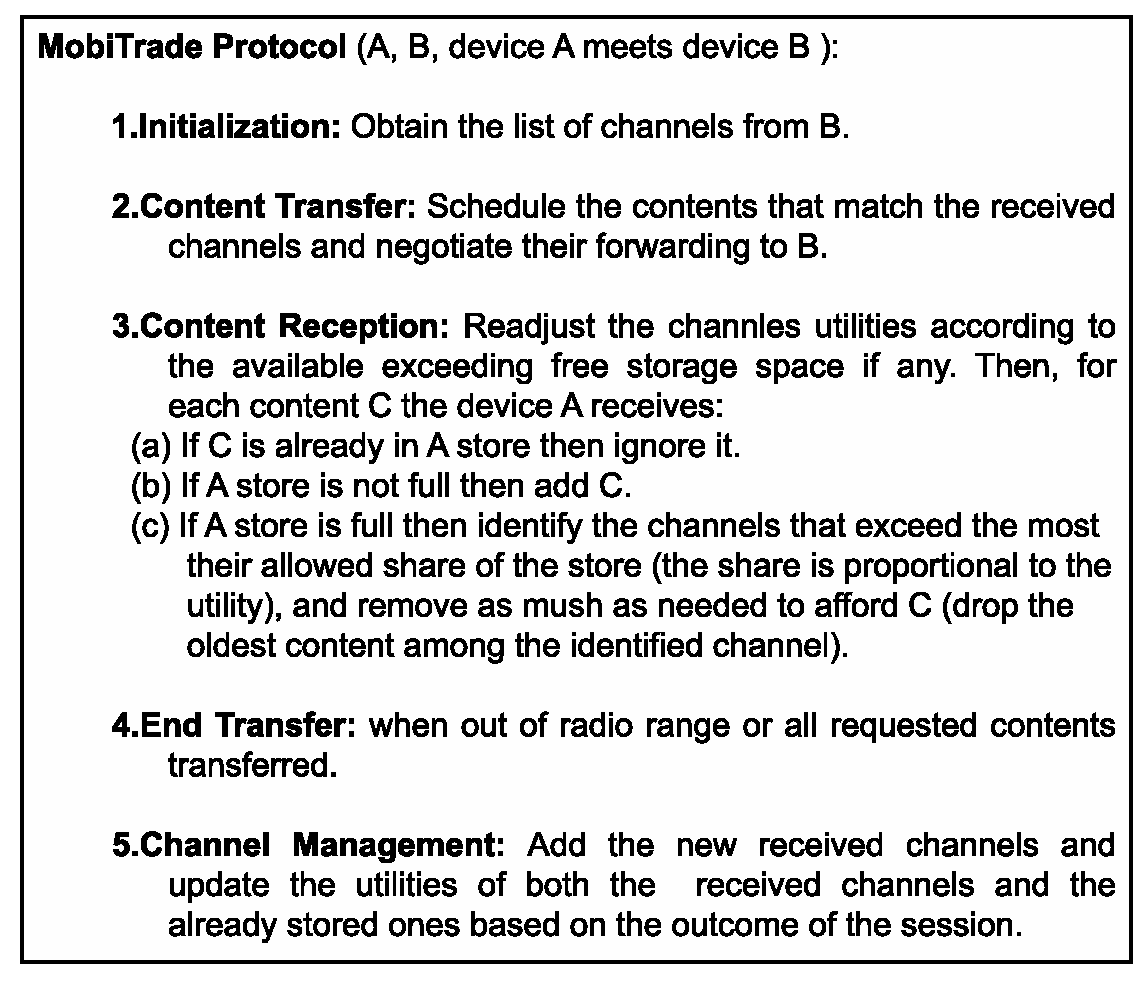
\includegraphics[width=3.5in,height=3in]{Chapitre5/MobiTrade-Protocol.eps}
\vspace{-0.1in}
\caption{MobiTrade protocol}
\label{protocol}
\vspace{-0.1in}
\end{figure}

\subsection{Tit-For-Tat Trading}
\label{contents-trading-scheduling}

One major difference of our system compared to other content dissemination solutions for DTNs (e.g.~\cite{May07wirelessopportunistic,ContentPlace,TACODTN}) is that we assume that participating users are selfish by default. Thus they might act as free-riders: during a meeting they receive content they want but don't give something back (even if they have), in order to save transmission power or to save some bandwidth. Or, they might not collect content their peers are requesting. Experience teaches us that even in the absence of power or storage concerns (e.g. wired users of BitTorrent), additional concerns (legal, malice), might motivate users to circumvent collaborative mechanisms~\cite{BitThief}. We believe these are \emph{powerful incentives that could sabotage any collaborative content dissemination system, if not properly handled}.

In order to remedy this and isolate selfish users, a \emph{strict} Tit-For-Tat (TFT) trading is enforced during meetings. Content scheduled for exchange is forwarded one-by-one (or in equally sized blocks/pieces, if contents are not of equal size), i.e. node A sends some, then node B sends some, then node A again, etc. Forwarding of content stops when the other device cannot (or chooses not to) reciprocate the amount of bytes it received\footnote{In order to solve the bootstrapping issue, when two well-intended devices meet for the first time, MobiTrade enables generous cooperation up to a certain amount as described in Section~\ref{managing-channels}.}. 

In addition to this TFT mechanism ensuring that selfish nodes are not serviced when content for them \emph{is} available, a utility maintenance mechanism (to be described in Section~\ref{managing-channels}) further ensures that well-intended nodes will not waste their resources collecting content for selfish nodes from which they will not receive any reward.


\section{Inference of Channel Utility}
\label{managing-channels}

MobiTrade aims at maximizing the number of collected contents while providing incentives for devices to collaborate. To have their requests satisfied, MobiTrade devices have to propose contents to other devices in counterpart of what they are looking for. As said before, each device is equipped with a storage space that is filled with contents from the different existing channels, which are used later as trading currency. This storage space is filled so as to satisfy the future demand: each channel occupies a proportion of the storage equal to the reward it is expected to bring upon future meetings. Due to Tit-For-Tat trading, the reward from carrying a channel is the amount of data from this channel a device will sell upon future meetings (to get both data for its own usage and data used for later trading). Hence, \emph{to optimize performance, MobiTrade devices should be able to quantify the expected reward from the channels they carry.}

In MobiTrade, the expected reward from each channel is modeled through a utility function used for ranking contents upon a meeting and for dropping them upon saturation of the storage. In this section, we detail how these utilities are calculated. Table~\ref{table:notation} summarizes some useful notation.

\begin{table}
\vspace{-0.1in}
\caption{Notation}
\centering
\label{table:notation}
\footnotesize
\begin{tabular}{|p{2cm}||p{10cm}|}
\hline
\bfseries Variable & \bfseries Description\\
\hline
$U_{CH}(n)$ & In bytes. Models the utility of the channel $CH$ at the $n_{th}$ meeting.\\
\hline
$X(CH)$ & 0 or 1. Expresses whether the met device is also interested in channel $CH$ or not.\\
\hline
$CL(CH)$   & In bytes. Expresses the collaboration level of the met device during a given meeting with respect to the channel $CH$.\\
\hline
$SC(CH)$   & In bytes. Expresses the number of bytes sent to the met device during a given meeting with respect to the channel $CH$.\\
\hline
$\omega$ & Between 0 and 1. A weight that decides on the elapsed time window over which we average the utility of channels.\\
\hline
$\alpha$ & In bytes. Expresses MobiTrade device generosity level, used to de-block the situation when two devices meet for the first time and request new channels.\\
\hline
$\beta$ & In bytes. Controls the speculation that a MobiTrade device makes regarding the expected future reward from a given channel.\\
\hline
\end{tabular}
\end{table}

For each channel $CH$, MobiTrade defines its utility $U_{CH}(n)$ at the $n^{th}$ meeting (counted over all devices) in a way to reflect the \emph{expected} number of bytes the device will sell from this channel (and thus the bytes of interest these will buy back) with any random device it will meet\footnote{Note that MobiTrade does not differentiate between own and foreign channels (these could also overlap) at the level of calculating utilities. However, foreign content doesn't interfere with content for own consumption. If a peer has content of interest for own consumption, this will always be retrieved, provided it can be ''bought'', and passed to the application. MobiTrade only decides whether this should be further cached in the content storage for future trading.}. This is clearly a complex interplay of mobility patterns, available channels and content, and node interests. \emph{We choose to keep our framework as assumption free as possible about mobility and interest patterns}, and take the following approach.

\noindent \textbf{Calculation and update of channel utilities:}
Assuming stationarity of the network over at least a time window of $2T$, the expected reward from carrying a channel $CH$ can be calculated by averaging all experienced rewards over all meetings in the past time window $T$. Meetings that do not request channel $CH$ count as zero. To facilitate implementation, an Exponential Weighted Moving Average (low pass) filter is used for averaging.

Let's consider a device $A$ and let's suppose that an $(n+1)^{th}$ meeting opportunity arises. After the establishment of the physical connection, both devices exchange matching contents while applying the Tit-For-Tat trading algorithm (as in Figure~\ref{protocol}). Once done, they both record the volume of exchanged data and update each the utilities of the channels they carry. For device $A$ and channel $CH$, this update is done as follows:
\begin{eqnarray*}
U_{CH}(n+1) = \omega . U_{CH}(n) + (1 - \omega) . X(CH) . CL(CH),
\label{eq:utility-updating}
\end{eqnarray*}
where $\omega = (t_{n}-t_{n-1})/T$ is the weight associated to the low pass filter\footnote{By making it function of the elapsed time between the current meeting and the previous one, one can ensure an averaging over a time window $T$.}. Concerning the term on the right hand side, it models the amount of data exchanged with the met device $B$ from channel $CH$. $X(CH)$ is a binary variable that expresses whether $B$ is interested or not in $CH$. This variable captures the popularity of a given channel over all MobiTrade devices met by $A$. As for $CL(CH)$, it captures the volume of contents that could be sold to device $B$ in the future (i.e. a prediction of $B$'s future demand for $CH$).

This calculation leads to several nice properties. First, this utility calculation is per channel and does not account for the physical addresses of encountered devices. The same device met several times or different devices met the same number of times count the same from the viewpoint of MobiTrade, as long as the amount of data sold was the same. This avoids tracking individual devices which improves the scalability of MobiTrade. Second, it does not try to over-optimize for the next meeting only (as could be the case with detailed mobility prediction) but rather optimizes the inventory over a larger time horizon, enough to absorb prediction inaccuracies at individual meetings. Finally, coupled with the Tit-For-Tat algorithm, our utility (through $CL(CH)$) accounts for the collaboration of devices in addition to the popularity of channels. In lack of this feature, a channel widely requested among a group of users, who do not collaborate by bringing back interesting contents for $A$, could force $A$ to keep collecting contents matching $CH$, only to discover later that this content buys him nothing. The storage of $A$ could have been better used by carrying contents for less popular channels but more collaborative devices.

\noindent \textbf{Collaboration and Bootstrapping:}
The $CL(CH)$ term above expresses the collaboration level of the device $B$ with respect to the channel $CH$. If a channel however is requested for the first time at the $(n+1)^{th}$ meeting, its $U_{CH}(n)$ would be initialized to zero. A new node that asks for a channel $CH$, would see its request being ignored, as no content for $CH$ was exchanged in this round. Clearly, an appropriate bootstrapping mechanism is needed, in order to avoid this chicken and egg problem for new nodes or channels. This can be implemented as some \emph{slack} or \emph{generosity} in the $CL(CH)$ calculation and the TFT mechanism. At the same time, this generosity should be such that it \emph{cannot be exploited} by selfish nodes. The calculation of $CL(CH)$ below is inspired from TCP slow start, and attempts to best satisfy the above two (conflicting) goals:

$$
CL(CH) = \left\{
    \begin{array}{ll}
        Max(\alpha, 2 . SC(CH)) & \mbox{if } SC(CH) < \beta, \\
        SC(CH) + \alpha & \mbox{otherwise.}
    \end{array}
\right.
$$
The collaboration level $CL(CH)$, that is, the prediction of future demand, is thus a function of the actual (last exchange) demand $SC(CH)$. If $SC(CH)$ is less than some threshold $\beta$, we allow $SC(CH)$ to double, to accelerate the collaboration process at its beginning; otherwise, devices will have to meet more often to reach a satisfactory collaboration level. After $\beta$\footnote{We take an optimistic approach and choose it equal to the maximum utility value over all channels of $A$.}, the generosity of device $A$ switches into a linear mode when it believes it has successfully approximated the steady-state demand, and only speculates an additional $\alpha$ to $SC(CH)$.

The same factor $\alpha$ is equally used as minimal value for $CL(CH)$ to unblock the situation when device $B$ asks for a new channel ($SC(CH)$ equals zero in this latter case). If a channel does not bring the expected reward for any reason (lack of collaboration, oldness of the contents carried, etc.), this will be reflected by a decrease in $SC(CH)$, which automatically leads to a decrease in the utility value we associate to this channel. Similarly, $\alpha$ also serves to keeps selfish nodes in control. If some selfish device asks for a long list of new channels, MobiTrade will associate initially a small utility value to them. A selfish/malicious user is then obliged to collaborate in order to increase the utilities of his channels and thus the portion of content storage these are given.

From the perspective of a collaborative trader node, a community of non collaborative users is equivalent to a community of users not requesting channels. We believe this improves the robustness of the system and allows it to scale to large networks, without the need for explicit blacklisting and reputation systems (at least for selfish nodes).

%Another feature of setting $CL(CH)$ this way is the ability to protect collaborative users from non collaborative ones. Indeed, a selfish user requesting channels but not collaborating with the other devices will see its $SC(CH)$, and hence its $CL(CH)$, set to low values. The result will be almost equivalent to this user not requesting any channel ($X(CH)$ set to zero). 

\section{Performance Evaluation}
\label{performance-evaluation}

We move now to performance evaluation of our system. We first describe our experimental setup, and then present simulations results for two main types of scenarios: collaborative scenarios and scenarios including selfish users.

\subsection{Experimental Setup}
\label{experimental-setup}

\emph{Protocols:} We have implemented the MobiTrade content dissemination protocol in the NS3 simulator~\cite{NS3}. Throughout our simulations we will be considering two versions of MobiTrade, with (\textbf{MobiTrade + TFT}) and without Tit-For-Tat (\textbf{MobiTrade - TFT}). Note that this corresponds only to the forwarding module, described in Section~\ref{contents-trading-scheduling}. The channel utility maintenance, described in Section~\ref{managing-channels}, is kept on in all scenarios. We have also implemented two different versions of the \emph{podnet07} scheme as a baseline for comparison\footnote{We choose the PodNet framework, as it is the most directly comparable to our scheme, and consists of simple enough mechanisms that we consider practical for implementation. For example, \cite{OptimalChannelChoice} is considerably more complex and based on an MCMC framework that requires careful simulated annealing and might take a long time to converge. Furthermore, \cite{ContentPlace} requires explicit knowledge of social network links, not available in our framework.},  as described, to our best understanding in~\cite{May07wirelessopportunistic} and~\cite{Podcasting:Secon07}: (i) non-collaborative Podcasting, where users just carry and share their own channels~\cite{May07wirelessopportunistic} (\textbf{Podcasting}); (ii) collaborative Podcasting with the \emph{Uniform} channel sharing strategy, where, a device records all channels it has seen in the past and solicits contents for these channels randomly~\cite{Podcasting:Secon07} (\textbf{Podcasting + Uniform}). This latter strategy was shown to perform best in~\cite{Podcasting:Secon07}, compared to other heuristics taking into account channel popularity. As a final note, we stress that MobiTrade's first goal is not to compete with optimal collaborative schemes, but rather to efficiently deal with selfish nodes, without compromising the socially optimal (collaborative) performance.

\emph{Mobility Models:} To evaluate the different protocols, we use two type of mobility scenarios, a state-of-the-art synthetic mobility model (HCMM)~\cite{HCMM} and a real mobility trace (KAIST)~\cite{KAIST}. HCMM is a mobility model inspired by Watts' Caveman model that was shown to reproduce statistics of human mobility, such as inter-contact times and contact duration. In HCMM, the Caveman model is used to define a graph (overlay) with nodes divided into (well connected) groups and each group is assigned to a physical home location. Also, some users belonging to different groups can have links to each other (bridges). These (intra- and inter-group) links are used in HCMM to drive movements: each user moves towards a given group's home location with a probability
proportional to the weight of its links towards the group. In our scenario, we consider 50 users distributed into 5 groups. The plane is divided into a 10*10 grid of cells (5000 m wide), and each cell can serve as a home location for a group.

The KAIST scenario consists of real human mobility traces collected from a university campus (KAIST) in South Korea~\cite{KAIST}. We consider a sample of the KAIST campus traces taken from 50 students, where the GPS receivers log their position at every $30$ seconds. We integrated both mobility models in NS3. Both case studies consist of simulations that last $24$ hours where devices use the $802.11b$ protocol to communicate with a transmission range around $60$ meters.

\emph{Traffic Model:} Unless otherwise stated, each user joins randomly $2$ channels at the beginning of the simulation. For simplicity, we assume that all generated contents have the same size\footnote{Variable sized content could still be split to equal sized pieces or blocks. We defer the study of more complex content structures to future work.}. However, different channels do not need to have the same size (the size of a channel is equal to the sum of its contents' sizes). Some channels might have lots of content, and others less. Finally, we consider that each user generates contents periodically that match one of the channels that were requested by users from other groups\footnote{The content generation interval depends on the number of contents for a channel and the duration of the simulation.}.

\subsection{Collaborative scenarios}
\label{collaborative-scenario}

We first evaluate MobiTrade, assuming all nodes are collaborative, using the following four scenarios (described in Table~\ref{table:c-sim-sce}) (there are $50$ channels in total): {$\mathbf{SC_1}$} implements a \emph{homogeneous traffic} pattern, i.e. each channel has the same size and each user joins the same number of channels. In $\mathbf{SC_2}$, users choose a \emph{random number of channels} to join, but channels still have the same size. In $\mathbf{SC_3}$, users ask for the same number of channels but these have \emph{random sizes}. Finally, $\mathbf{SC_4}$ introduces some \emph{churn}, where $10$ of the users join the simulation after $8$ hours, while existing sessions are ongoing, and leave again $8$ hours later. Due to space limitations, for all scenarios, we show plots for the HCMM mobility model, accompanied with respective results for the KAIST trace summarized in Tables.

\begin{table}[!h]
\vspace{-0.1in}
\caption{Collaborative simulation scenarios}
\centering
\label{table:c-sim-sce}
\footnotesize
\begin{tabular}{|p{3cm}|p{2cm}|p{2cm}|p{2cm}|p{2cm}|}
\hline
\bfseries Sim. Scenario: & $\mathbf{SC_1}$ & $\mathbf{SC_2}$ & $\mathbf{SC_3}$&  $\mathbf{SC_4}$ \\
\hline
\bfseries Nbr. of Users: & 50 & 50 & 50 & 40 + 10 transient\\
\hline
\bfseries Requested CH(s) per User & 2 & random [1, 20]& 2& 2\\
\hline
\bfseries Size of CH(s) (\# of contents) &20  &20 &Random [1, 20]&20 \\
\hline
\end{tabular}
\end{table}

\noindent \textbf{Effect of TTL:} Before we proceed, we take a quick look first into the impact of content TTL. As explained in Section~\ref{MobiTrade-architecture}, our buffer drop and scheduling policies give priority to younger messages\footnote{Note that this age \emph{only} corresponds to the time the content was inserted in the network by its publisher, and does not (directly) relate to the actual age (e.g. an old vs. a new rock song.)}. This is not only in accordance with our daily experience (for many types of content, e.g. news feeds, we prefer to have the most recent version), but has also been shown to be an efficient resource allocation policy in the context of a single channel~\cite{TMC:Report} (intuitively, older content has a higher chance to have been delivered already). Figure~\ref{DO} depicts the MobiTrade average delivery rate as a function of the content $TTL$ (for scenario $\mathbf{SC_1}$), with and without prioritizing younger messages (per channel). It is evident that the higher the (application chosen) $TTL$ the more old content ``hogs'' node buffer and contact bandwidth, not allowing new content to reach its audience. When prioritizing younger messages, not only does performance stabilize, but with an infinite TTL the gain from just this mechanism is up to $76\%$.

\begin{figure}[!h]
  \begin{center}
    \includegraphics[width=3in,height=2.2in]{Chapitre5/fig3.eps}
  \end{center}
  \caption{Drop and Scheduling policy inside the same channel ($\mathbf{SC_1}$).}
  \label{DO}
\end{figure}

\begin{figure}[!h]
  \begin{center}
    \includegraphics[width=3in,height=2.2in]{Chapitre5/fig5.eps}
  \end{center}
  \caption{Fixed number of channels per user and fixed channel size ($\mathbf{SC_1}$).}
  \label{CS+FNC+FCS}
\end{figure}

\noindent \textbf{Scenario} $\mathbf{SC_{1}}$: Figure~\ref{CS+FNC+FCS} compares the performance of MobiTrade with and without TFT and the two versions of Podcasting described in Section~\ref{experimental-setup}. The figure of merit is, again, the average delivery rate, defined as the \emph{amount of content received for channels a node requested} divided by the \emph{total amount of content generated for these channels} (throughout the simulation). This is averaged over all nodes. Delivery rate is plotted as a function of node storage.

There are three main observations to be made in Figure~\ref{CS+FNC+FCS}. \emph{First}, collecting and sharing foreign channels (\textbf{MobiTrade} and \textbf{Podcasting + Uniform}) improves performance compared to only storing own channel. This confirms the findings of~\cite{Podcasting:Secon07}. \emph{Second}, the uniform sharing policy~\cite{Podcasting:Secon07} is clearly not optimal (as suggested also in~\cite{OptimalChannelChoice}), and is significantly outperformed by MobiTrade's inventory management (by up to $2 \times$). This is more pronounced as storage is increased. \emph{Third}, using Tit-For-Tat (TFT) in a context where \emph{all} nodes are well-intended results in a small drop of the average delivery rate by about $6\%$, compared to the case without TFT. Using game theoretic terms, in Section~\ref{game}, we show that \emph{rational users will choose to pay this price to secure themselves from selfish users}. Finally,  Table~\ref{table:kaist:col}, summarizes the respective results for the KAIST trace (we only show values for a buffer of $110$ contents; the plot trend is similar to Figure~\ref{CS+FNC+FCS}). The results for the KAIST trace (row 1) corroborate the above findings.

\begin{figure}[!h]
  \begin{center}
    \includegraphics[width=3in,height=2.2in]{Chapitre5/fig4.eps}
  \end{center}
  \caption{Scenario $\mathbf{SC_2}$.}
  \label{CS+RNC+FCS}
\end{figure}

\begin{figure}[!h]
  \begin{center}
    \includegraphics[width=3in,height=2.2in]{Chapitre5/fig7.eps}
  \end{center}
  \caption{Scenario $\mathbf{SC_3}$.}
  \label{CS+FNC+RCS}
\end{figure}


\begin{table}[!h]
\vspace{-0.1in}
\caption{Avg. delivery rate based on the real KAIST trace (collaborative scenario, content storage size = 110 contents).}
\centering
\label{table:kaist:col}
\footnotesize
\begin{tabular}{|p{3cm}|p{2cm}|p{2cm}|p{2cm}|p{2cm}|}
\hline
\bfseries Policy:& \bfseries MobiTrade + TFT & \bfseries MobiTrade - TFT & \bfseries Podcasting & \bfseries Podcasting Uniform\\
\hline
\bfseries Scenario $\mathbf{SC_{1}}$ & 0.83 & 0.89&0.6 &0.72\\
\hline
\bfseries Scenario $\mathbf{SC_{2}}$ & 0.78 &0.86 &0.75 &0.69\\
\hline
\bfseries Scenario $\mathbf{SC_{3}}$ &0.79  &0.88 &0.68 &0.74\\
\hline
\end{tabular}
\end{table}

\noindent \textbf{Scenarios} $\mathbf{SC_{2}}$ and $\mathbf{SC_{3}}$: These two scenarios consider the effect of heterogeneity with respect to channel demand ($\mathbf{SC_{2}}$) and channel size ($\mathbf{SC_{3}}$). The goal is to examine whether \emph{asymmetry} of demand or supply of content (common in practice) could give rise to \emph{deadlocks} due to the \emph{inherent symmetry} of the Tit-For-Tat mechanism.

Figures~\ref{CS+RNC+FCS} and~\ref{CS+FNC+RCS} show the respective delivery rate for these two scenarios, as a function of storage space. As we can see, traffic asymmetry does not affect the main observations made in scenario $\mathbf{SC_{1}}$. Interestingly,  for ($\mathbf{SC_{2}}$), Podcasting only own channels seems to outperform uniform sharing of foreign channels. Results for the KAIST trace are again in agreement (rows 2 and 3 of Table~\ref{table:kaist:col})). We conclude that, even in the presence of asymmetric traffic, MobiTrade performs up to almost $2\times$ better even without selfish nodes. Finally, while it is clear that these two scenarios do not suffice to \emph{exclude} every probability of a deadlock, they constitute positive evidence to the robustness of MobiTrade. We defer an analytical treatment of deadlocks to future work.


\noindent \textbf{Scenarios} $\mathbf{SC_{4}}$: The objective of this last scenario is to study the impact of \emph{node churn} and the ability of MobiTrade to efficiently bootstrap new nodes. Here, $10$ new users join the simulation after $8$ hours, each one of them asks for $2$ already existing channels, then, it leaves the simulation $8$ hours later. Figure~\ref{10-new-users} plots the average delivery rate among the $10$ new users and the $40$ existing ones as a function of time.
It is evident there, that when the new set of users join already existing channels, they are not blocked. Instead, they are able to collaborate and quickly scale up their performance\footnote{The important thing in this plot is the slope of the curves for new and old nodes, which matches, implying that both types get 
similar service. They differences in absolute value are only because nodes joining late have already missed part of the content already generated for this channel (and possibly dropped due to congestion).}.

\noindent \textbf{Delay:} Finally, in Figure~\ref{avg-delay}, we look at the average delivery delay of different schemes (scenario $\mathbf{SC_{1}}$), measured as \emph{time a matching content is received} $-$ \emph{time it was inserted in the channel}. We can clearly see that the ranking of schemes in terms of delay is similar to the one for delivery ratio (Figure~\ref{CS+FNC+FCS}).

\begin{figure}[!h]
  \begin{center}
    \includegraphics[width=3in,height=2.2in]{Chapitre5/fig8.eps}
  \end{center}
  \caption{Scenario $\mathbf{SC_4}$, 10 new users ask for already existing channels.}
  \label{10-new-users}
\end{figure}

\begin{figure}[!h]
  \begin{center}
    \includegraphics[width=3in,height=2.2in]{Chapitre5/fig12.eps}
  \end{center}
  \caption{Scenario $\mathbf{SC_1}$, studying the average delivery delay.}
  \label{avg-delay}
\end{figure}

\subsection{Scenarios with selfish users (SU)}
\label{selfish-scenario}

Having established the good performance of MobiTrade in the absence of selfish nodes, we now turn our attention to scenarios where few or more nodes might not reciprocate for content they receive. We deem such scenarios as the norm rather than the exception in the real world. As mentioned earlier, most related proposals do not deal (explicitly) with such users. We consider two such scenarios, as described in Table~\ref{table:m-sim-sce}: In $\mathbf{SS_{1}}$, we consider $10$ selfish users among $50$ that ask for different channels than those requested by the remaining collaborative users. In $\mathbf{SS_{2}}$, we consider the same number of selfish users which ask randomly for channels already requested by collaborative users. Selfish users and Collaborative users are denoted with ``SU'' and ``CU'', respectively.

\begin{table}[!h]
\vspace{-0.1in}
\caption{Simulation scenarios including selfish users.}
\centering
\label{table:m-sim-sce}
\footnotesize
\begin{tabular}{|p{3cm}|p{4cm}|p{4cm}|}
\hline
\bfseries Sim. Scenario: & $\mathbf{SS_1}$ & $\mathbf{SS_2}$\\
\hline
\bfseries Nbr. of Users: & 40 CU + 10 SU & 40 CU + 10 SU\\
\hline
\bfseries Nbr. of CH(s) & CU: 2/20 - SU: 2/10 (SU and CU channels differ) & CU, SU: 2/20 (among same channels) \\
\hline
\bfseries Size of CH(s) & CU: 20 - SU: 40  & CU, SU: 20 \\
\hline

\end{tabular}
\end{table}

\noindent \textbf{Scenario} $\mathbf{SS_1}$:  Figure~\ref{SS-Scenario-1} depicts the average delivery rate (for different user strategies, CU and SU) with and without the TFT mechanism enabled. At high congestion (storage of $50$ contents), enabling the TFT mechanism increases the average delivery rate among collaborative users by $15\%$ ($16\%$ using the KAIST trace, Table~\ref{table:kaist:mal}) and decreases it among selfish users by $63\%$. Indeed, enabling the TFT mechanism blocks selfish users and makes MobiTrade re-dispatch/reuse the saved resources among the channels shared by collaborative users. For a storage of $110$, collaborative users are able to reach  $73\%$ higher throughput than selfish ones, by using TFT. The latter see a $3-4\times$ drop in performance.  In the same context, as shown in Table~\ref{table:hcmm:vss}, the Podcasting scheme cannot control selfish nodes, as expected, and as their numbers increase, the latter end up outperforming collaborative ones. 

\noindent \textbf{Scenario} $\mathbf{SS_2}$: Here, the $10$ selfish nodes ask for channels already requested and carried by collaborative ones. This means that the utility management mechanism cannot affect them, allowing more opportunities to ``scrape'' content. Figure~\ref{MN+ECH+ICN} plots the average delivery rate of (MobiTrade + TFT) among collaborative users in two cases: first \emph{(i)}, when selfish users are active and second \emph{(ii)} when they are inactive. Clearly, when TFT is used, the performance of collaborative users is not harmed (verified also for the KAIST trace, Table~\ref{table:kaist:mal}), while the one of selfish users drops severely, by up to $2.1\times$ for a storage of $110$ contents\footnote{We observe that in this, as well as the previous scenario, selfish users are not $100\%$ isolated. This is \emph{only due} to the generosity mechanism described in Section~\ref{managing-channels} and the fact that we chose the minimum unit of transmission $\alpha$ to be one content, for simplicity. Increasing the amount of content in the network or reducing the value of $\alpha$ (note that this does not affect collaborative users much, due to the multiplicative increase), further isolates selfish nodes.}. This result consolidates our findings in Section~\ref{managing-channels} regarding the impact of selfish users on the performance of collaborative ones once they both join the same channels. Indeed, selfish users are simply considered by MobiTrade as users which don't ask for the channels. The system resources are kept safe and only dispatched among collaborative users.

\begin{figure}[!h]
  \begin{center}
    \includegraphics[width=3in,height=2.2in]{Chapitre5/fig1.eps}
  \end{center}
  \caption{Scenario $\mathbf{SS_1}$, impact on selfish and collaborative users.}
  \label{SS-Scenario-1}
\end{figure}

\begin{figure}[!h]
  \begin{center}
    \includegraphics[width=3in,height=2.2in]{Chapitre5/fig6.eps}
  \end{center}
  \caption{Scenario $\mathbf{SS_2}$, impact on collaborative users.}
  \label{MN+ECH+ICN}
\end{figure}

\begin{table}[!h]
\vspace{-0.1in}
\caption{Avg. delivery rate based on the real KAIST trace (scenario including selfish users, content storage size = 50 contents).}
\centering
\label{table:kaist:mal}
\footnotesize
\begin{tabular}{|p{1.5cm}|p{2.5cm}|p{2.5cm}|p{2.5cm}|p{2.5cm}|}
\hline
\bfseries Policy:& \bfseries MobiTrade (CU) & \bfseries MobiTrade (CU)& \bfseries MobiTrade + TFT(SU) & \bfseries MobiTrade - TFT(SU)\\
\hline
$\mathbf{SS_{1}}$: & 0.79 (+TFT)& 0.68 (-TFT) & 0.21& 0.57 \\
\hline
$\mathbf{SS_{2}}$: & 0.81 (+TFT, Inactive SU) & 0.78 (+TFT, Active SU) &0.24&0.77\\
\hline
\end{tabular}
\end{table}

\begin{table}[!h]
\vspace{-0.1in}
\caption{Avg. delivery rate (HCCM mobility model, content storage size = 110 contents, CU and SU ask for different channels).}
\centering
\label{table:hcmm:vss}
\footnotesize
\begin{tabular}{|p{5cm}|p{0.8cm}|p{0.8cm}|p{0.8cm}|p{0.8cm}|}
\hline
\bfseries Nbr. SU(s):& $\mathbf{5}$ & $\mathbf{10}$& $\mathbf{15}$ & $\mathbf{20}$\\
\hline
\bfseries MobiTrade + TFT(CU): & 0.8 & 0.76 &0.71 &0.62 \\
\hline
\bfseries MobiTrade + TFT(SU): & 0.25 & 0.22 &0.2&0.17\\
\hline
\bfseries Podcasting + Uniform(CU): &  0.46&0.4 &0.37&0.34\\
\hline
\bfseries Podcasting + Uniform(SU): & 0.29&0.33&0.36&0.39\\
\hline
\end{tabular}
\end{table}

\subsection{Choosing Strategies in MobiTrade}
\label{game}

We have so far considered scenarios with $x$ collaborative nodes or $y$ selfish ones. But why would any node choose to be selfish or collaborative? Our results suggest that selfish behavior pays off if other nodes have TFT off, but hurts when TFT is on. And why would a collaborative node choose to employ our TFT mechanism? Our results suggest that \emph{if all nodes are collaborative} they might get more content by turning TFT off. When multiple nodes have with these choices, where would the system converge? We \emph{sketch} below a game theoretic framework that tries to answer these questions (due to space limitations, we don't include here a more rigorous treatment).

Let's consider a simple case of two nodes with contents to exchange. The set of strategies $\mathcal{A}$ for each node is to choose from is: (i) being selfish (SU), (ii) being collaborative while activating TFT (CU + TFT) or (iii) being collaborative but not activating TFT (CU - TFT). Let $M$ be the amount of content these nodes get if they normally use MobiTrade (CU+TFT). Let finally $\gamma$ be a \emph{discount factor}, capturing the cost to a node (e.g. energy) of reciprocating a piece of content ($ 0 \le \gamma \le 1$).  The \emph{total payoff} to each node from getting $M$ contents is
\begin{eqnarray*}
payoff = \gamma M.
\end{eqnarray*}
The following matrix describes the ``MobiTrade game'' and the respective payoffs in normal form. It is not a zero-sum game.

\begin{table}[!h]
\vspace{-0.1in}
\caption{MobiTrade Game and Payoffs.}
\centering
\label{table:game}
\footnotesize
\begin{tabular}{|p{2cm}|p{2cm}|p{3cm}|p{3cm}|}
\hline
\bfseries & \bfseries CU + TFT & \bfseries CU - TFT  & \bfseries SU\\
\hline
\bfseries CU + TFT & $[\gamma M, \gamma M]$ & $[\gamma M^{+}, \gamma M]$ & $[0,0]$\\
\hline
\bfseries CU - TFT & $[\gamma M, \gamma M^{+}]$ & $[\gamma M^{+}, \gamma M^{+}]$ &$[(\gamma - 1) M^{+}, M^{+} ]$ \\
\hline
\bfseries SU &$[0, 0]$ &$[ M^{+}, (\gamma - 1) M^{+}]$ & $[0, 0]$\\
\hline
\end{tabular}
\end{table}

We note that $M^{+}$ is the somewhat higher payoff a node gets if both nodes are not selfish and disable TFT (see e.g. Figure~\ref{CS+FNC+FCS}) and $(\gamma - 1)M (\le 0)$ is the cost to a node of sending $M$ contents without getting something back. We can see that if $\gamma = 0$ (cost per content is equal to gain), then no user has an incentive to participate in the system (i.e. users will be selfish). This however, as well as $\gamma = 1$, are unrealistic cases.

The more interesting cases are for $0 < \gamma < 1$. In this case, it is easy to see that the game has a single \emph{Nash equilibrium} at (CU + TFT, CU + TFT) with payoffs ($\gamma M, \gamma M$). That is, none of the two nodes can \emph{strictly} improve its payoff by a \emph{unilateral} change of strategy~\cite{game}. In other words, for nodes participating in our network choosing to use MobiTrade with TFT is the optimal (selfish or rational) strategy, which is a very desirable outcome for out system. This analysis can be easily extended to $N$ nodes. The main difference there is that (CU+TFT) has a non-zero reward even if all but one other users are not SU (making the equilibrium stronger).

Finally, deactivating TFT, i.e. point (CU-TFT, CU-TFT), is the socially optimal operating point and is also \emph{Pareto optimal}. However, it is not an equilibrium except for the limiting case of $\gamma = 1$ (no cost). For all other cases, the \emph{price of anarchy} per node is equal to $\gamma (M^{+} - M)$, which as we saw in the results of this section, is only a small price to pay.

\section{Summary and Open Issues}

In this chapter, we investigated the content dissemination problem over DTN while considering the possible existence of selfish users.
Inspired from real life trading behavior, we proposed MobiTrade, a complete framework that incites users to collaborate, profiles their needs and manages their device resources optimally towards maximizing their revenues in terms of contents. Using NS3 simulations based on a synthetic mobility model (HCMM), and a real mobility trace (KAIST), we show that selfish users are isolated and system resources are only allocated among collaborative users. Finally, using a game theoretic framework, we show that turning on MobiTrade is the optimal strategy to use for selfish, rational users. In future work, we intend to consider more complex content structures (e.g. hierarchical channels, semantic matching, etc.) and their effect on our system.

\chapter{MobiTrade: Implementation on Android Platform}
\label{chapter:MobiTrade}
\minitoc

We present in this chapter the software design of the MobiTrade application for opportunistic collaborative content sharing that we have implemented for the android platform. We follow a top-down description approach. We start by giving a high level overview of the MobiTrade application architecture and its design principles in Section~\ref{MobiTradeArchitecture} namely MobiTrade functional blocks, followed by a description of the mobile application architecture and the content sharing session. Then, we dig deeper into the network and link level technical details of the MobiTrade android application in Section~\ref{MobiTradeDesignAndImplementation}. In Section~\ref{MobiTradeCurrentFunctionalities}, we describe through screen shots the set of functionalities actually provided by MobiTrade~\cite{MobiTradeAndroid}. Finally, we conclude this chapter with a discussion of the open issues and a summary in Section~\ref{MobiTradeSoftSummary}.

\section{MobiTrade Architecture Overview}
\label{MobiTradeArchitecture}

\subsection{MobiTrade Functional Architecture}
\label{MobiTrade-functional-architecture}

Having described MobiTrade algorithms in Chapter~\ref{chapter:PTMP}, we give here some more details on the MobiTrade functional architecture that encapsulates the latter algorithms. Figure~\ref{MobiTrade-node-architecture} is a schematic of MobiTrade functional architecture which encapsulates 5 building blocks:

\begin{figure}[!h]
\centering
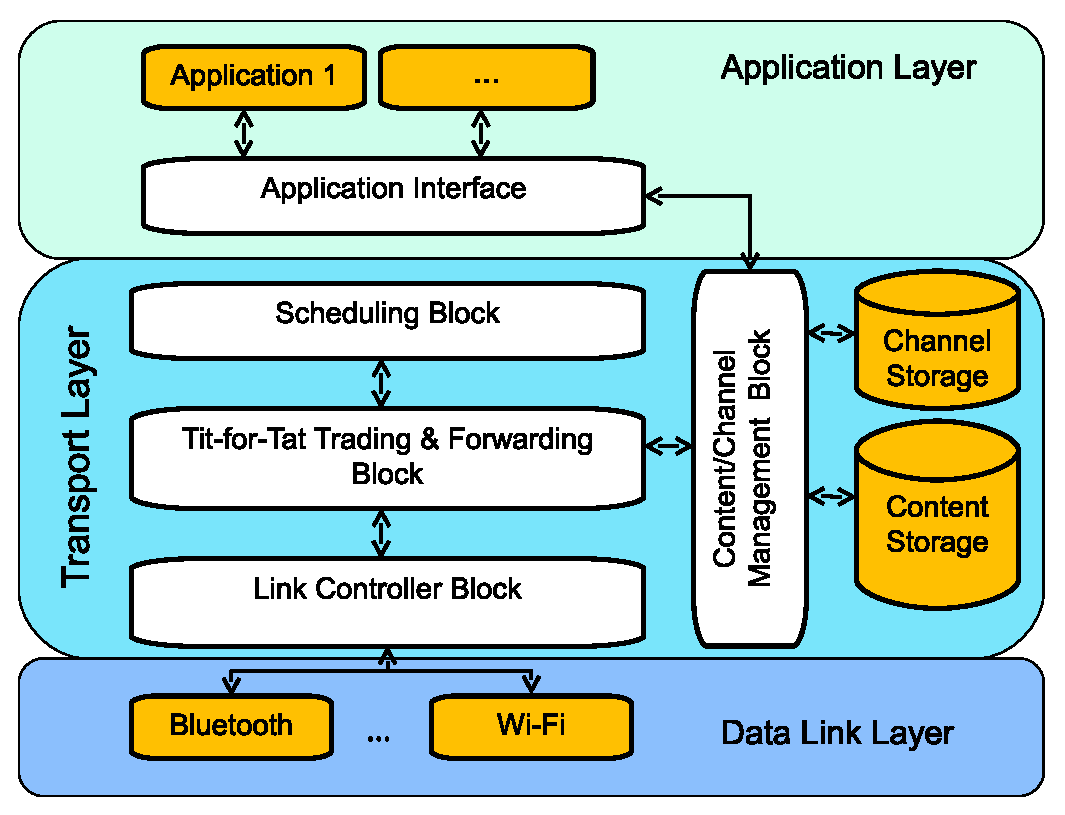
\includegraphics[width=3.5in,height=3in]{Chapitre6/MobiTrade_Node.eps}
\caption{MobiTrade protocol functional building blocks}
\label{MobiTrade-node-architecture}
\end{figure}

The \textit{Application Interface} is designed so that developers can easily extend MobiTrade and create new content sharing applications that use the MobiTrade functionalities. Each MobiTrade application has a unique ID that it registers at the application interface. The application then simply communicates with the MobiTrade system using event handlers.

The \textit{Scheduling Block} defines the order to follow while forwarding a set of requested contents within a limited contact opportunity. This ordering is done based on the matching channels utility values.

The \textit{Tit-For-Tat Trading and Forwarding Block} takes in charge the forwarding of the stored channels records whenever a new contact is established, and the negotiation and forwarding of the requested contents.

The \textit{Content/Channel Management Block} manages the channel and content storage space. It provides an API for storing and retrieving channel and content records that hides the storage technology specifics. This block also takes in charge utility updates for the stored channels and buffer management.

The \textit{Link Controller Block} is the lowest layer in the MobiTrade architecture. It provides a common interface for sending and receiving data across the different available wireless interfaces. It is also responsible for periodically scanning the neighborhood for devices, for establishing the contacts whenever meeting opportunities arise and for triggering the Tit-For-Tat trading and forwarding block. The link controller provides an API that hides network technology specifics (Bluetooth or Wi-Fi) from the rest of the upstream blocks.

\subsection{MobiTrade Android Device Model}
\label{MobiTrade-device-model}
 
Here, we cast the functional architecture described in the latter section within the android platform in order to figure out the right device model and to identify the suitable technical components. 

As we have described before in the previous Chapter, the MobiTrade architecture relies on user collaboration and on a content trading scheme in order to maximize user revenues in terms of content of interest to him. Whenever a user expresses his interest on a given channel and unless he is already connected to other users that can immediately provide the contents he is interested, the user cannot expect to get an immediate answer to its content request. Instead, the common behavior will consist on the fact that the MobiTrade application will keep running in background for an amount of time (could be long) in order to to able to exploit any future possible meeting opportunity and try to get back the content its local user is looking for. In short, the user should be able to express his interests, head out in the real world and wait to get notified whenever a content of interest is retrieved.  In order to fulfill such a need and as described in Figure~\ref{MobiTrade-application}, we choose to encapsulate the MobiTrade functional blocks already described in the previous section within an android service which has the capabilities to keep running in background even if the user is not interacting with the MobiTrade application. At the same time, we developed a separate graphic user interface based on android activities in order to provide to the user a full control of the running service if needed. Indeed, as described in Figure~\ref{MobiTrade-application}, from within the MobiTrade user interface, the user has access to four different tabs that mainly enable him to request channels, publish contents, explore existing channels and contents, tune MobiTrade algorithms configuration, etc. We will provide later in this chapter more details about theses different tabs through real screen shots.

The MobiTrade android application supports also a set of advanced notifications which could be easily tuned by the user via the configuration tab function of its needs. As described in Figure~\ref{MobiTrade-application}, these notifications are triggered by the MobiTrade service (running in background) and translated by the android Notifications Manager API into either a personalized device physical vibration or text message exposed to the user via the SmartPhone notification bar. 

\begin{figure}[!h]
\centering
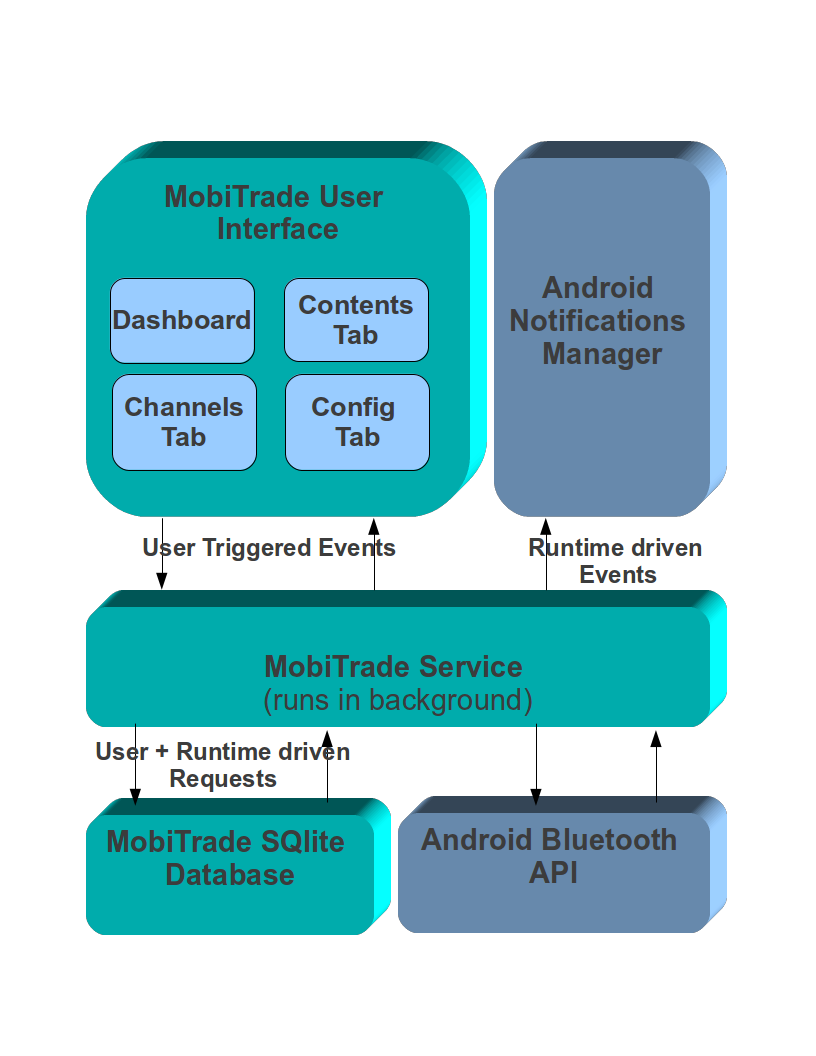
\includegraphics[width=3.5in,height=3in]{Chapitre6/MobiTradeCommunicationArchitecture.png}
\caption{MobiTrade Device Model}
\label{MobiTrade-application}
\end{figure}

Since MobiTrade is based on \emph{store-carry-and-forward} content sharing approach, nodes should be able to efficiently store channels records as well as their associated contents. Also, in the context of time/bandwidth limited contacts, MobiTrade application should also be able to identify and extract efficiently the list of contents that match a set of received channels records in order to answer the remote device upon a MobiTrade session. Convinced that the latter needs could be fully satisfied by a relational database engine and taking into consideration the fact that the selected engine should be supported by our target platform (android), we choose to work with an SQLite database engine. Indeed, an SQLite~\cite{SQLite} database requires little or no administration, it is a good choice for devices or services that must work unattended and without human support. SQLite is a good fit for use in SmartPhones and it works very well as an embedded database in applications. So, as described in Figure~\ref{MobiTrade-application}, our MobiTrade mobile application uses and SQLite database engine for channels and contents records management.

With regards to the underlying wireless technology we choose to initially base our implementation on Bluetooth technology rather than on Wi-Fi but, we also intend to support the Wi-Fi in ad hoc mode in the future. Indeed, the current android Java libraries do not support the ad hoc mode of Wi-Fi although this is supported by both the driver and the hardware interface on almost android mobile devices. Therefore, making our implementation supporting the ad hoc mode requires the device to be run in privileged user mode (i.e. rooted mode) so that the interface can be reconfigured to run in ad hoc mode.

\subsection{MobiTrade Session}
\label{MobiTrade-session}

We mean by a MobiTrade session the protocol followed by a pair of mobile devices following a successful meeting and a wireless (Bluetooth) connection establishment. Figure~\ref{mobitradesession} depicts a UML (Unified Modeling Language) sequence diagram that describes in details the dynamics of a MobiTrade session between two devices $A$ and $B$. 

As described in Figure~\ref{mobitradesession}, the MobiTrade session is triggered by the device A that starts by serializing the channels records that it stores locally into an XML message (described in Figure~\ref{channelsxml}) then, it sends the serialized message through the established Bluetooth channel towards the remote peer. Once received, the channels XML record is parsed within the device B using an XML SAX parser~\footnote{There are many XML parsers that are available. Choosing a right one for a situation might be challenging. Only three XML parsing techniques are extremely popular and are used for Java. Document Object Model (DOM), is W3C provided mature standard, and simple API for XML (SAX), it was one of the first to be widely adapted form of API for XML in Java and has become the standard. The third one is Streaming API for XML (SAX), which is a new model for parsing in XML but is very efficient and has a promising future. Each one of the mentioned techniques has their advantages and disadvantages. Choosing the right technique depends mainly on the application, its requirements and the hosting device capabilities. We choose to use a SAX parser since it is an event-driven parser that does not need to build the entire tree describing the XML document within memory and hence it does not require lot of memory space which is something we try to minimize within MobiTrade.}. The latter device extracts the channels attributes (keywords, utilities ...) and decides based on them of the set of contents that could be of interest to the device A. Once the later contents are identified, MobiTrade schedules them based on the utilities of their matching channels and prepares them for forwarding upon a possible request from the TFT block. At the mean time, the device B serializes also its locally stored list of channels and sends them back to the device A. The latter follows the same steps as done by device B in order to identify any possible matching content. Once done, the MobiTrade protocol triggers the TFT algorithm within device A in order to run and manage the contents exchanging process. The TFT block serializes the first scheduled content into an XML message (described in Figure~\ref{contentxml}) and forwards the latter one to device B which in return decides of the content to forward back based on the size of the received one. The TFT process continues until one of the devices or both of them exhaust their list of scheduled contents. 

\begin{figure}[!h]
\begin{center}
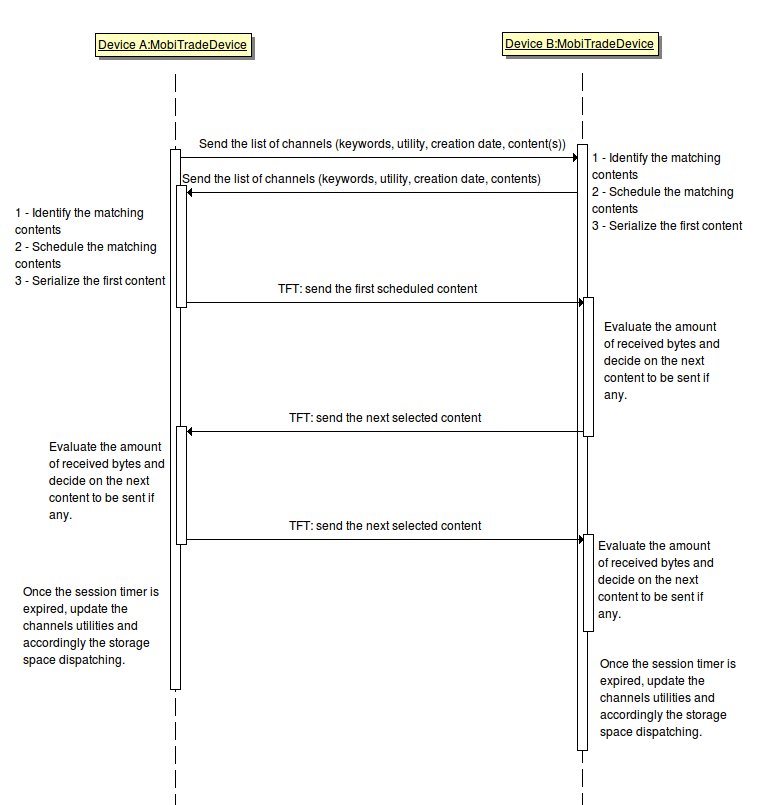
\includegraphics[width=5in,height=6in]{Chapitre6/MobiTradeSession.png}
\end{center}
\caption{MobiTrade session.}
\label{mobitradesession}
\end{figure}

\begin{figure}[!h]
\begin{center}
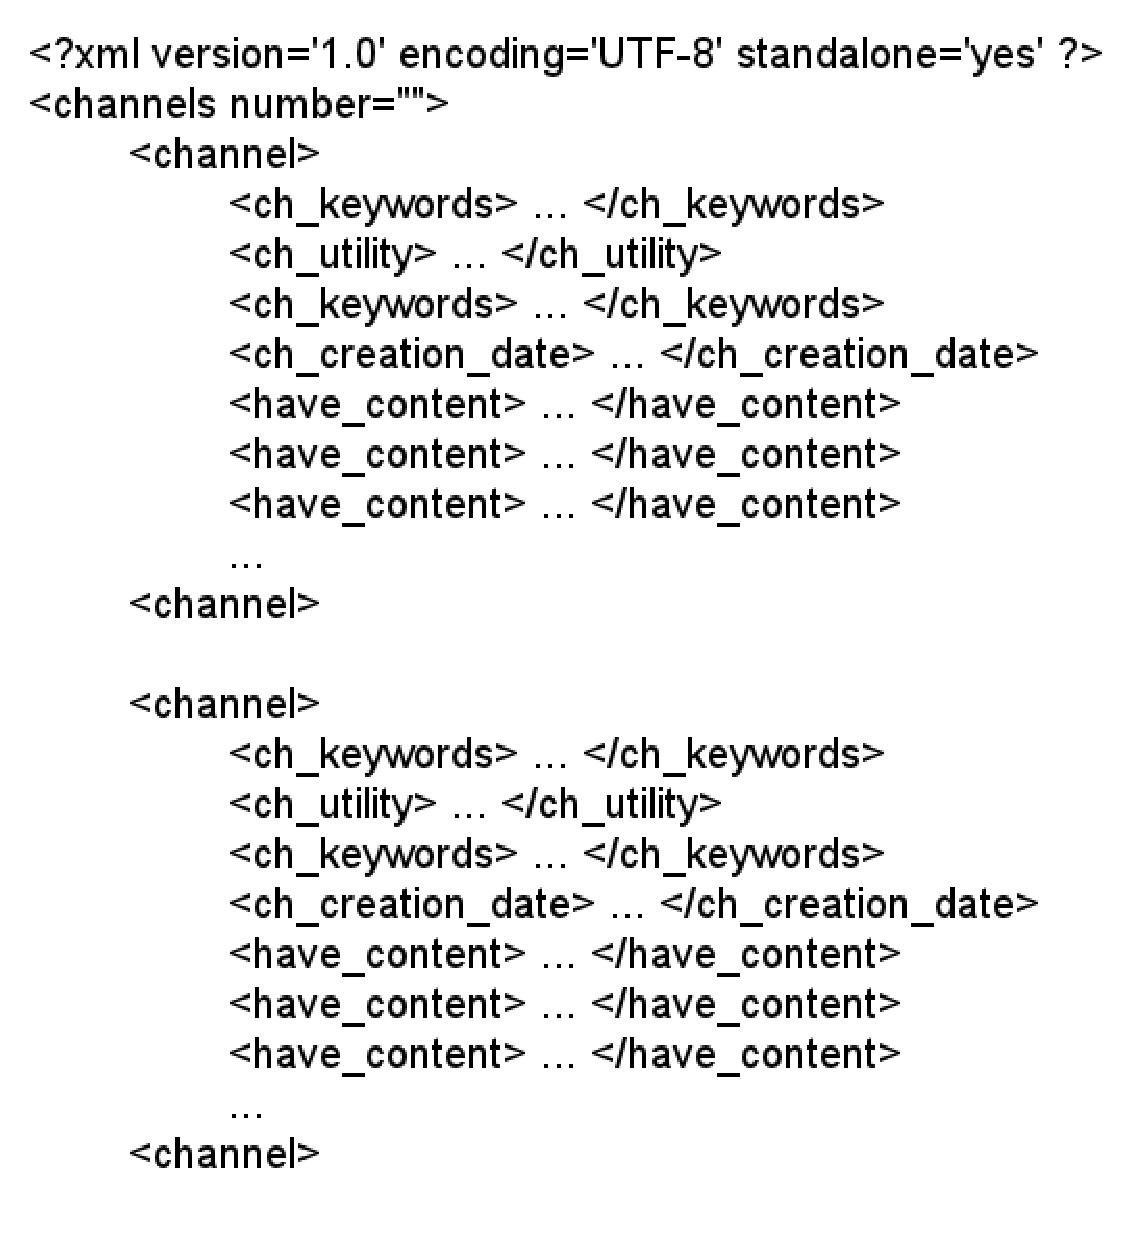
\includegraphics[width=4in,height=3in]{Chapitre6/channelsxml.eps}
\end{center}
\caption{Channels xml description.}
\label{channelsxml}
\end{figure}

In order to simplify the MobiTrade session and to make it as more efficient as possible, we choose to serialize also the content binary data within the XML document (see Figure~\ref{contentxml}). It is true that XML is not the ideal carrier for binary data. It is a text format, and as such does not cope well with raw bits. But, if binary data is properly encoded, using something like the W3C XML scheme types Base64Binary, then using the XML converters reading and writing binary files becomes a snap. So, in our case, we use the Base-64 encoding/decoding format in order to be able respectively to include the content binary data as an element within the XML document (see Figure~\ref{contentxml}) at the sender side and to extract it at the receiver one.  

\begin{figure}[!h]
\begin{center}
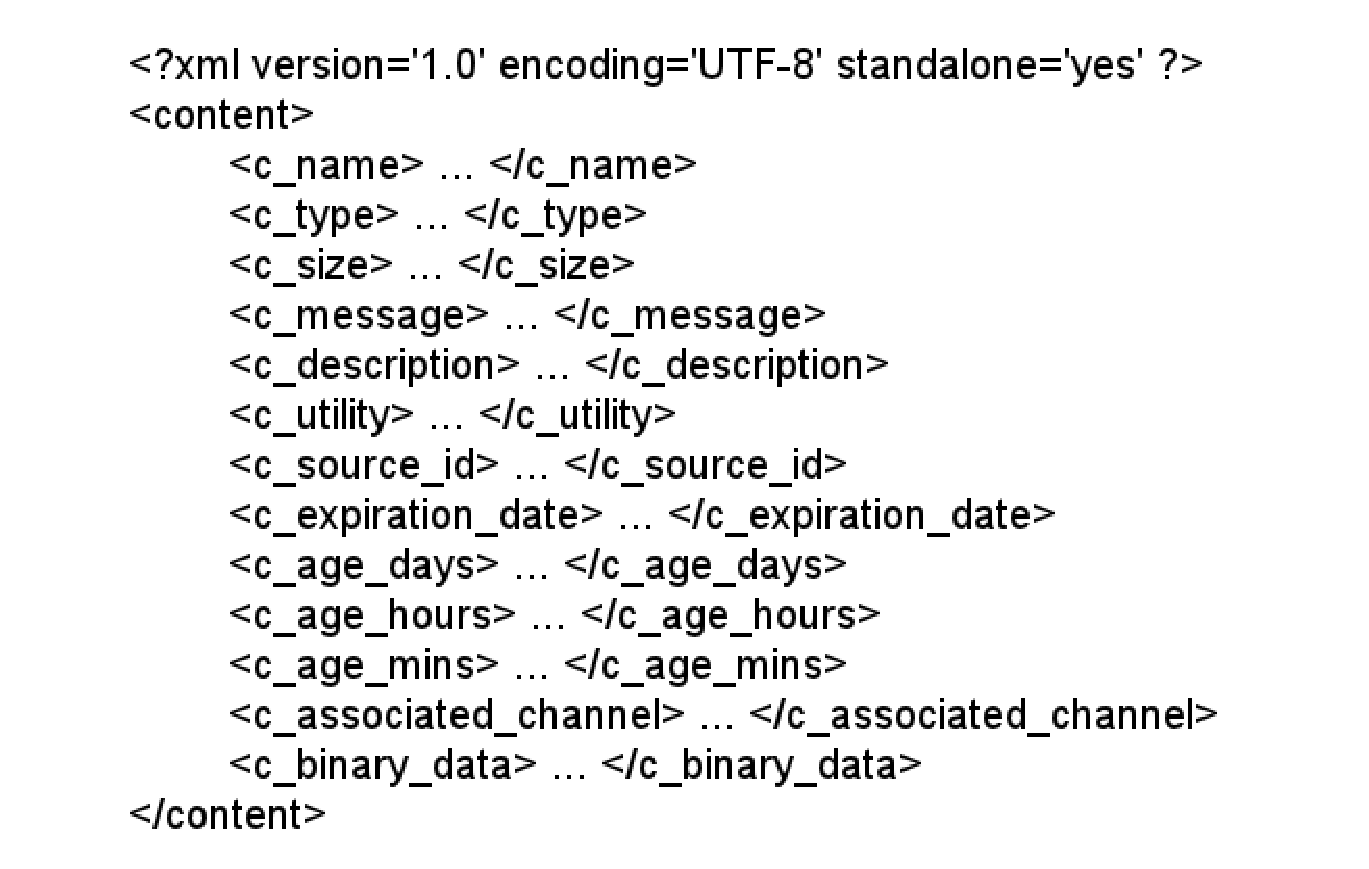
\includegraphics[width=4in,height=3in]{Chapitre6/contentxml.eps}
\end{center}
\caption{Content XML description.}
\label{contentxml}
\end{figure}

\section{MobiTrade Support for Bluetooth}
\label{MobiTradeDesignAndImplementation}

As explained before, we choose to initially base our implementation only on Bluetooth technology since the current android Java libraries do not support the ad-hoc mode of 802.11. Bluetooth is a low-power short-range wireless communication technology intended to replace the cables connecting electronic devices. Below we give a short overview on the Bluetooth protocol stack, the device discovery procedure (called inquiry scan in Bluetooth terminology), supported higher layer protocols and the application programming interfaces.

\subsection{Bluetooth Overview}

Bluetooth operates on a license-free ISM band at 2.4GHz (the same as used by 802.11). The physical layer is based on frequency hopping spread spectrum (FHSS) and transmits data on up to 79 frequency bands (1 MHz each). Each frequency band is divided into time slots and full duplex transmission is provided through the use of a time-division duplex (TDD) scheme.

Bluetooth network has a master-slave structure. A master device can communicate with up to seven devices forming a so called piconet. In a piconet devices communicate on the same physical channel that is defined by a common clock (set by the master) and a frequency hopping pattern. By definition, the device that initiates a connection becomes the master. Once a piconet has been established, master-slave roles may be exchanged. At any given time, data can be transferred between the master and one other device, but never directly between two slaves. A device can only be synchronized to a single channel at a time. Multiple simultaneous operations (e.g. participating in various piconets, being discoverable and connectable) are supported using time-division multiplexing between various channels. However, device can only be the master of a single piconet.

Above the physical layer in the architecture there is a number of logical links for control and data traffic. These are managed by a L2CAP layer that provides a channel based abstraction for applications. One logical (and physical) link can thus carry data for multiple applications. L2CAP provides reliable transmission performing flow control, CRC checks and retransmissions upon request. The main traffic services provided are asynchronous connection-oriented unicast and isochronous constant rate channel (e.g. for audio streaming). However, these channels are rarely used directly by applications; instead several higher layer protocols have been standardized and implemented in various client libraries. 

The most commonly adopted Bluetooth specifications include v1.2, v2.0 and v2.1 all being backwards compatible. The specifications differ mainly in supported bit rates and support for some advanced features. The nominal rate for Bluetooth v1.2 is 1Mbit/s. Bluetooth v2.0 increases the bit rate up to 2Mbit/s (Basic Rate) and 3Mbit/s (Enhanced Data Rate or EDR). v2.1 extends the inquiry responses (more on this below) and adds secure pairing among other minor tweaks. The operational ranges of Bluetooth devices vary from approximately 1, 10 to 100 meters (class 3, class 2 and class 1 respectively). Smartphones are generally class 2 devices.

\paragraph*{Inquery Scan Procedure}

The Bluetooth specification defines two separate physical channels for device discovery (inquiry scan channel) and connection setup (page scan channel).  Each Bluetooth devices can be in one of the four states: (i) connectable and discoverable, (ii) connectable, (iii) discoverable, or (iv) neither discoverable nor connectable. A device cannot be discovered nor connected unless it is configured in the correct state.

A discoverable device listens for inquiry requests periodically (called inquiry scan state) on its inquiry scan channel that has a reduced number of hop frequencies and a slower rate of hopping. In order to discover neighboring devices, an inquiring device hops through all possible inquiry scan channel frequencies in a pseudo-random fashion, sending an inquiry request on each frequency and listening for responses. This is done at a faster rate, allowing the inquiring device to cover all inquiry scan frequencies in a reasonably short time period. The Bluetooth specification recommends an inquiry duration of 10.24s. Then, with high probability, all neighboring devices will have entered their inquiry scan state and will hear the inquiry.

An inquiry response consists of a unique 48-bit device address of the discovered device and a 24-bit Class-of-Device code (CoD). The CoD consists of a major and minor device codes. The device codes are standardized and provide information about the device type: major code can tell if the device is a computer or a phone for example while the minor code can specify if the device is a cellular or cordless phone. In addition, each device may have a human readable name that can be queried using a separate control request. The extended inquiry response available in v2.1 can provided the human readable name and additional information about supported services directly in the inquiry response. Older Bluetooth devices must use the separate control request and a service discovery protocol (see below) instead.

Once a device is discovered, a connection setup can take place. A connectable device is listening on its page scan channel for connection requests that are sent in a similar fashion as inquiry scans. The connection setup must be completed before any data can be transmitted between the devices.

\paragraph*{Higher Layer Protocols}

Each Bluetooth device must support the Service Discovery Protocol (SDP). The service discovery mechanism provides the means for client applications to discover the existence of services provided by server applications as well as the attributes of those services. The attributes of a service include the type or class of the service and the protocol information needed to access the service. The SDP protocol itself is run by a SDP server on the device that is responsible of maintaining the local service records and answering service discovery queries for SDP clients on other Bluetooth devices.

The Bluetooth specifications define various specialized protocols on top of the L2CAP layer for different purposes such as audio streaming, telephony and data transmissions. The most commonly used serial data stream protocol is RFCOMM. The RFCOMM protocol provides emulation of serial ports (up to 60 ports can be used simultaneously depending on the implementation). It provides a simple reliable data stream service, similar to TCP. In order to connect to another Bluetooth device over RFCOMM, the client must know the server channel which can be resolved using SDP. It is also possible to use hard-coded channels, but dynamic channel numbers are recommended since the number of available channels is very limited (30). 

Our MobiTrade android implementation makes use of the service discovery protocol (SDP) and establishes an RFCOMM serial data stream in order to efficiently run a given MobiTrade session and to exchange the needed meta-data messages as well as the contents themselves. According to MobiTrade architecture, each mobile device plays at the same time the role of a client and a server. So, it hosts a MobiTrade service which in return will accept and manage incoming connections and supports needed functionalities in order to initiate and run a MobiTrade session. Indeed,  using SDP, a MobiTrade device has the ability to identify whether the remote peer hosts a MobiTrade service or not. If a running service is discovered, then, the mobile device establishes an RFCOMM channel with the remote peer in order to exchange the needed messages.    

\paragraph*{Application Programming Interfaces}

The main interface between user level applications and the Bluetooth device is called Host Controller Interface (HCI) that is standardized in the Bluetooth specification. However, existing Bluetooth protocol stack implementations typically do not allow direct access to the HCI interface but provide their own abstractions of the main Bluetooth operations. The main stacks in use include BlueZ for Linux based devices 2, Windows Bluetooth stack and WinSock for Windows and Windows CE based devices 3 and Broadcom's Bluetooth stack for Windows based devices 4.

The client APIs let the applications control the device state (discoverable and/or connectable), the human readable Bluetooth device name and very often the CoD value. The device inquiry can be initiated at anytime through the Bluetooth API and the applications can typically control the duration of the inquiry and/or the number of responses to wait for. The applications can also query for the human readable names of the discovered devices, create local SDP records for the services they provide and query the records of nearby devices. The data services such as RFCOMM are typically accessed using a special type of socket and the familiar socket API.

\subsection{Android Platform Support for Bluetooth}

Since the android platform is based on a Linux kernel, the provided android Bluetooth API is nothing but a Java wrapper around the Linux BlueZ stack. These APIs let applications wirelessly connect to other Bluetooth devices, enabling point-to-point and multi-point wireless features. Using the Bluetooth APIs, an android application can perform the following:

\begin{itemize}
\item Scan for other Bluetooth devices
\item Query the local Bluetooth adapter for paired Bluetooth devices
\item Establish RFCOMM channels
\item Connect to other devices through service discovery
\item Transfer data to and from other devices
\item Manage multiple connections
\end{itemize}

More details about the android Bluetooth API that we used for the development of the MobiTrade application are provided in~\cite{AndroidBluetoothAPI}. 

\section{Functionalities provided by the MobiTrade Android Application}
\label{MobiTradeCurrentFunctionalities}

The current android implementation of MobiTrade provides to the user a simplified dashboard (see Figure~\ref{dashboard}) from which he can both follow and interact on real time with the MobiTrade service. Indeed, the user have access to the current device Bluetooth state (whether the adapter is on or off, whether it is in discoverable mode or not and whether the device is currently running a discovery session or not). A set of statistics are also presented within the dashboard like the total number of contents stored within the device, the \% of used space with respect to the total space allocated to the MobiTrade application, the total number of channels maintained within the system, how much among the latter ones the user requested locally and finally the number of Bluetooth discovered devices that run MobiTrade.
 
\begin{figure}[!h]
\begin{center}
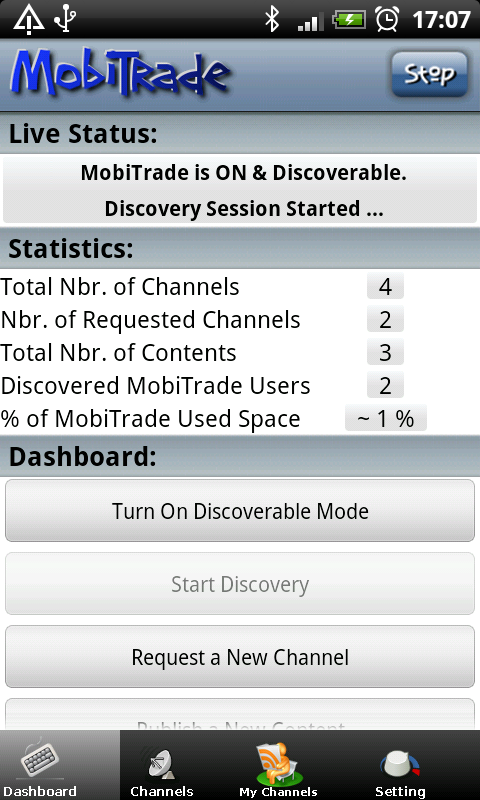
\includegraphics[width=2in,height=3in]{Chapitre6/Dashboard.png}
\end{center}
\caption{MobiTrade dashboard.}
\label{dashboard}
\end{figure}

In terms of functionalities, from within the dashboard depicted in Figure~\ref{dashboard}, the user is able to control the device Bluetooth discoverability, to control 
the Bluetooth discovery session, to manage channels (create new ones or join existing ones) and contents (create new contents or publish existing ones). We detail in the following paragraphs the latter functionalities.

\paragraph{Bluetooth Interface Management}

One of the limitations that we faced along the implementation of MobiTrade was related to the android Bluetooth stack. Indeed, there
was no way to keep the mobile device discoverable to other non paired devices for more than 300 seconds. Enabling discoverability is necessary for MobiTrade to host a server socket that will accept incoming connections, because the remote non paired devices must be able to discover the device before it can initiate the connection. According to the android SDK, by default, enabling discoverability makes the device discoverable for $120$ seconds. The android SDK provides a way to define a different duration by adding the \emph{EXTRA\_DISCOVERABLE\_DURATION} Intent extra, however the maximum duration is fixed to 300 seconds.

In order to overcome the latter limitation, we have added a broadcast receiver to MobiTrade to catch android Bluetooth scan mode changements. Then, whenever the scan mode changes to not discoverable the user is notified, so he can decide whether to re-enable discoverability or not. This could be done via the button \emph{"Turn On Discoverable Mode"} provided in the dashboard (see Figure~\ref{dashboard}).

Through the dashboard as well as the configuration tab described in Figure~\ref{Config}, we also provide to the user the control over the Bluetooth discovery sessions. Indeed, by default, whenever the MobiTrade service does not have a running content sharing session, it launches a Bluetooth discovery session trying to find new sharing opportunities. It is obvious that the latter behavior maximizes the probability of identifying new MobiTrade devices (sharing opportunities) however it can turn out very quickly to be a useless waste of energy (device battery). Indeed, if the user knows that he is going to be completely physically isolated from any possible sharing opportunity, he can decide to stop temporary the Bluetooth discovery mechanism and even the Bluetooth adapter itself towards saving some energy then, restart everything later. To do this, the user should ask MobiTrade to give him back control over the Bluetooth discovery mechanism by updating the corresponding entry in the configuration tab described in Figure~\ref{Config}. Then, the user can drive the discovery from within the dashboard (run it or stop it whenever needed).

\paragraph{Channels/Contents Management}

As describer in Chapter~\ref{chapter:PTMP}, MobiTrade manages autonomously the channels as well as their corresponding content records towards maximizing the revenues of the local user. At the same time, the current MobiTrade prototype provides to the user the possibility to interact and manage the set of locally stored channels/contents. Indeed, as described in Figure~\ref{JoiningNewChannel}, MobiTrade dashboard enables the user to ask for joining a new channel. The latter channel could be either an already discovered foreign channel (see Figure~\ref{JoiningExistingChannel} or a new channel that the user wants to create as depicted in Figure~\ref{CreatingNewChannel}.

\begin{figure}[!h]
\begin{minipage}[l]{0.3\linewidth}
\centering
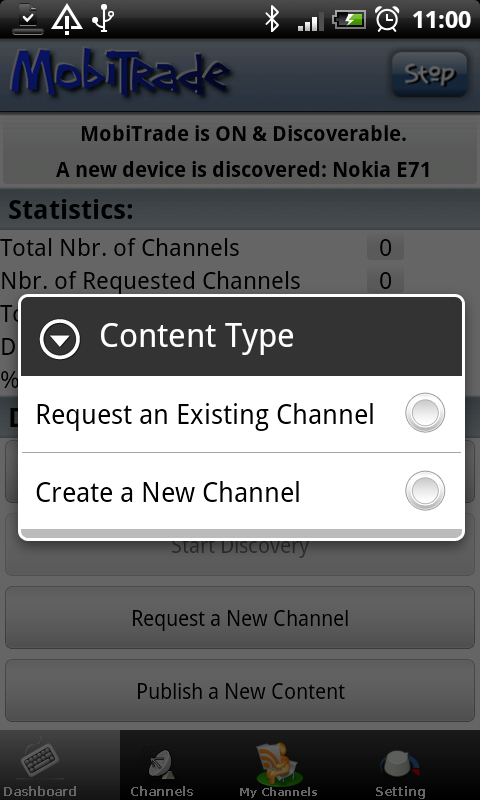
\includegraphics[width=2in,height=3in]{Chapitre6/JoinChannel.png}
\begin{minipage}[l]{1\linewidth}
\small
\caption{MobiTrade: Joining a new channel.}
\normalsize
\label{JoiningNewChannel}
\end{minipage}
\end{minipage}
\hspace{2.1cm}
\begin{minipage}[l]{0.3\linewidth}
\centering

\includegraphics[width=2in,height=3in]{Chapitre6/JoinExistingChannel.png}
\begin{minipage}[l]{1\linewidth}
\caption{MobiTrade: Joining an existing channel.}
\label{JoiningExistingChannel}
\end{minipage}
\end{minipage}
\end{figure}

The channels tab described in Figure~\ref{ListAllChannels} enables the user to navigate through the available channels: the foreign channels that MobiTrade decides to collect and maintain locally for future trading as well as the locally requested ones. All the channel records are organized within a scrollable list which makes it easy for the user to navigate forward to the channels' corresponding contents (see Figure~\ref{ListAvailableContents}) and backward to the channels tab. Note that the locally requested channels are also presented apart in a separate tab (see Figure~\ref{ListRequestedChannels}) which we think provides a quick access to the channels of local interest and their matching contents.

\begin{figure}[!h]
\begin{minipage}[l]{0.3\linewidth}
\centering
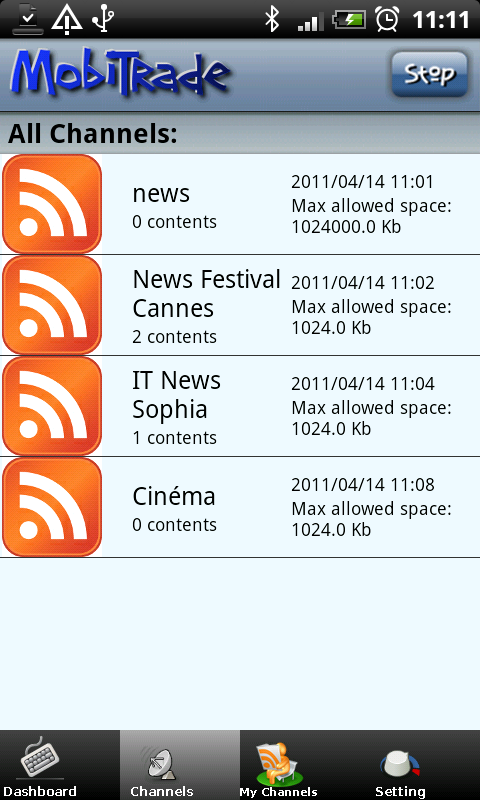
\includegraphics[width=2in,height=3in]{Chapitre6/ListAllChannels.png}
\begin{minipage}[l]{1\linewidth}
\small
\caption{MobiTrade: List of all channels.}
\normalsize
\label{ListAllChannels}
\end{minipage}
\end{minipage}
\hspace{2.1cm}
\begin{minipage}[l]{0.3\linewidth}
\centering
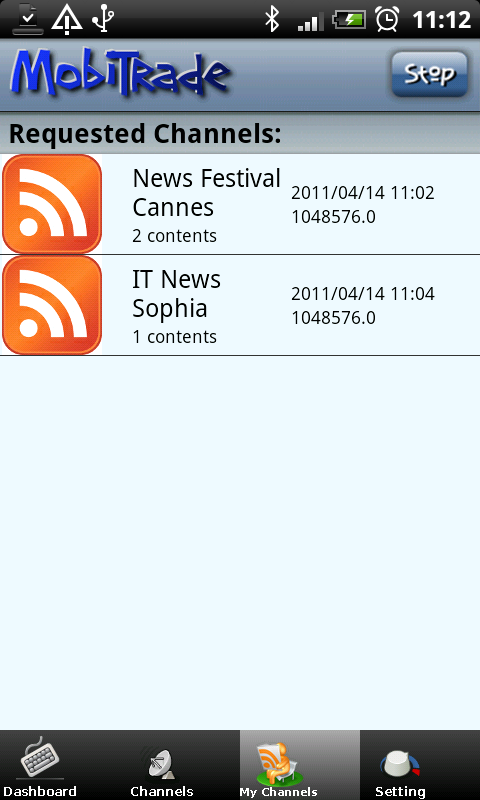
\includegraphics[width=2in,height=3in]{Chapitre6/ListRequestedChannels.png}
\begin{minipage}[l]{1\linewidth}
\caption{MobiTrade: List of locally requested channels.}
\label{ListRequestedChannels}
\end{minipage}
\end{minipage}
\end{figure}

From within the dashboard, the user is also able to publish a new content record. Once this task is initiated, the user is first asked to select the channel within which he wants to publish the new content. Then, as described in Figure~\ref{PublishNewContent}, the user can choose to either publish an existing content or create a new one (see Figure~\ref{CreatingNewContent}), and in both cases the user has to associate to the new content a short description which is used later by MobiTrade to run the matching process between the contents and the channels records.

\begin{figure}[!h]
\begin{minipage}[l]{0.3\linewidth}
\centering
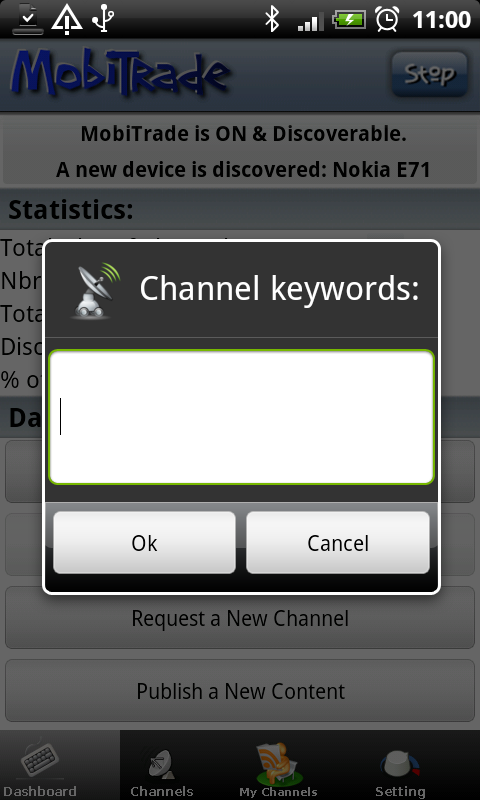
\includegraphics[width=2in,height=3in]{Chapitre6/CreateChannel.png}
\begin{minipage}[l]{1\linewidth}
\small
\caption{MobiTrade: Creating a new channel.}
\normalsize
\label{CreatingNewChannel}
\end{minipage}
\end{minipage}
\hspace{2.1cm}
\begin{minipage}[l]{0.3\linewidth}
\centering
\includegraphics[width=2in,height=3in]{Chapitre6/PublishContent.png}
\begin{minipage}[l]{1\linewidth}
\caption{MobiTrade: Publishing a new content.}
\label{PublishNewContent}
\end{minipage}
\end{minipage}
\end{figure}


\begin{figure}[!h]
\begin{minipage}[l]{0.3\linewidth}
\centering
\includegraphics[width=2in,height=3in]{Chapitre6/WriteMessage.png}
\begin{minipage}[l]{1\linewidth}
\small
\caption{MobiTrade: Creating a new content/message.}
\normalsize
\label{CreatingNewContent}
\end{minipage}
\end{minipage}
\hspace{2.1cm}
\begin{minipage}[l]{0.3\linewidth}
\centering
\includegraphics[width=2in,height=3in]{Chapitre6/ListContents.png}
\begin{minipage}[l]{1\linewidth}
\caption{MobiTrade: List of available contents with respect to the selected channel.}
\label{ListAvailableContents}
\end{minipage}
\end{minipage}
\end{figure}

\paragraph{MobiTrade Configuration}

As described in Figure~\ref{Config}, MobiTrade configuration tab provides to the user the possibility to tune some important parameters within the MobiTrade architecture. Namely, towards controlling the device resources usage (both local storage as well as battery), first it is made possible for the user to specify the maximum amount of storage space that MobiTrade is allowed to use both for storing locally requested contents as well as contents used for trading. And second, as described above in this section, the user can either leverage the control of the Bluetooth discovery sessions to MobiTrade service which will try to keep always discovering new sharing opportunities, or he can take the control over that process and decide the moment at which the device should run a discovery session. Following the latter option, the user can save lot of battery power without losing in terms of expected revenues from possible sharing opportunities.

Through the Configuration tab, the user also have the possibility the specify whether he wants or not to get notified via the device vibrator (if supported) whenever a new content that matches a locally requested channel is received. Indeed, this is a very interesting option because the user is not supposed to keep tracking on real-time the status of the content sharing sessions. Instead, the user can start MobiTrade service, choose to get notified, and then close the MobiTrade UI and head out on the real world. Whenever a new content of interest is received, the user is notified. Note that the MobiTrade UI is completely decoupled from the MobiTrade service in terms of \emph{life cycle}. MobiTrade UI could be down and at the same time MobiTrade service is running in background. Any time the user launches the MobiTrade activity (UI), he can control/follow on real time from within the dashboard what is going on with the MobiTrade service.

Note that MobiTrade configuration is maintained persistently within the mobile device. Thus, each time the user decides to update one of the configuration entries, he should validate the new configuration from within the tab. There will be always the possibility to re-load default configuration entries.

\begin{figure}[!h]
\begin{center}
\includegraphics[width=2in,height=3in]{Chapitre6/Config.png}
\end{center}
\caption{MobiTrade: Configuring the daemon.}
\label{Config}
\end{figure}

\section{Summary and Open Issues}
\label{MobiTradeSoftSummary}

We have described the design and implementation of our architecture for the Google android platform. Our experience from the implementation is that android is a very powerful platform and quite mature. The Java based environment provides a familiar environment with good support for most common OS primitives such as threads and concurrency, database and content storage and inter process communication through the android service binding mechanism. Some features are however still missing, in particular support for the 802.11 ad hoc mode (which needs to be implemented in native code). We believe that our design is general and facilitates the implementation of advanced content-centric applications. MobiTrade protocol and resources management policies can be easily customized which enables to quickly setup and evaluate various experimental scenarios. There are however some issues that are not, or only partially addressed by our design. We do currently not address particularly the issues of privacy, security and power management. The latter are one of our primary directions for future work. 


\chapter{Conclusions and perspectives}
\label{chapter:conclusions}

In this thesis, we have investigated the problem of mobile devices resources management towards setting up both efficient point-to-point content routing and dissemination within a delay tolerant network.
  
We first addressed the problem within the context of point-to-point DTN routing and proposed an optimal joint scheduling and buffer management policy (GBSD). We then introduced an approximation scheme (HBSD) for the required global knowledge of the optimal algorithm. Using NS2 simulations based on synthetic and real mobility traces, we showed that our policy based on statistical learning successfully approximates the performance of the optimal algorithm. Both policies (GBSD and HBSD) plugged into the Epidemic routing protocol outperform current state-of-the-art protocols like RAPID~\cite{Levine:Sigcomm07} with respect to both delivery rate and delivery delay, in all considered scenarios. Moreover, we discussed how to implement our HBSD policy in practice, by using a distributed statistics collection method, illustrating that our approach is realistic and effective. We also showed that, unlike related works~\cite{Levine:Sigcomm07, AOBM}, our statistics collection method scales well, not increasing the amount of signaling overhead during high congestion. We have also studied the distributions of HBSD utilities under different congestion levels and showed that the optimal policy heavily depends on the congestion level. The above findings suggest that methods to signal the congestion level could allow nodes to switch off the more sophisticated but \emph{heavier-duty} HBSD policy and use simpler local policies, when congestion is below some threshold. 

We then, investigated the large scale point-to-multipoint content dissemination problem over DTN while considering the possible existence of selfish users. We have first formulated the optimal content dissemination problem in DTNs from the perspective of non-altruistic nodes while relying on a \emph{tit-for-tat} mechanism to isolate free-riders. Then, we have proposed MobiTrade, a utility-based solution to this problem that predicts the (exchange) value of each piece of content and provides a customized resource allocation strategy for each node, matched to its own interests and mobility pattern. Finally, we have showed, using a game-theoretic framework that turning on MobiTrade leads to an efficient Nash equilibrium. To our best knowledge, MobiTrade is the first content sharing
system for DTNs that can both deal with rational and selfish users while at the same time achieving good global outcomes
without explicit hard constraints on the topology and dependency of nodes or on their social behavior. Indeed, MobiTrade establishes real life trading principles by inciting users to collaborate, profiling their needs and managing their device resources optimally towards maximizing their revenues in terms of contents. Using NS3 simulations based on a synthetic mobility model (HCMM), and a real mobility trace (KAIST), we showed that selfish users are isolated and system resources are only allocated among collaborative users. 

To consolidate the NS-2/NS-3 simulations, we implemented our HBSD and MobiTrade protocols respectively as an external router for the DTN2 reference platform and as standalone mobile application for the Android powered devices. HBSD real implementation is available on our web site \cite{HBSDDTN2}, users can easily download and deploy both the DTN2 platform along with the HBSD external router and tune latter if needed. With respect to MobiTrade, the Android mobile application prototype is available for download on our web site \cite{MobiTradeAndroid}. We detail in \cite{MobiTradeAndroid} the architecture as well as the features of the MobiTrade prototype. 

As a future work, and towards consolidation our proposal (HBSD) for the point-to-point content routing problem over DTN, it would be interesting to define buffer management and scheduling policies that take into account different messages sizes (in this work, we considered that all messages have the same size). For example, in case of congestion, the end-to-end delay versus message delivery trade-off could be influenced by the choice of dropping several small messages or one large message that occupies the entire node's buffer. Then, starting from our findings which state that 
the optimal policy heavily depends on the congestion level, another interesting future work direction would be to study and design an end-to-end congestion control scheme. Indeed, signaling the congestion level could allow nodes to switch off the more sophisticated but \emph{heavier-duty} HBSD policy and use simpler local policies, when congestion is below
some threshold. We believe that such a mechanism, if available, would enable mobile nodes to save lot of resources (energy, storage and contacts' bandwidth). The latter problem remains largely not addressed in the DTN context.

Then, with respect to our proposal (MobiTrade) for the point-to-multipoint content dissemination problem over DTN, we aim at implementing the MobiTrade protocol for other types of devices and experiment with real large scale communities of users, and hence it will be possible to study MobiTrade architecture scalability under real conditions. Furthermore, it would be interesting to consider more complex content structures and their effect on MobiTrade performance. Moreover, one can go one step further with the study of the needed mechanisms to control possible advanced malicious attacks and behaviors that could impair MobiTrade content sharing sessions. Such mechanisms could be easily integrated within MobiTrade channels' utilities.
    




\appendix

\chapter{Appendix Example}
\label{chap:appendix1}

\section{Appendix Example section}

And I cite myself to show by bibtex style file (two authors) \cite{Commowick_MICCAI_2007}.

This for other bibtex stye file : only one author \cite{Oakes_RStat_1999} and many authors \cite{Guimond_CVIU_2000}.

%\bibliographystyle{ThesisStyle}
\bibliographystyle{IEEEtran}
\bibliography{Thesis}

%\printnomenclature

\end{document}
